%!TEX root = ../thesis.tex
%*******************************************************************************
%****************************** Fourth Chapter *********************************
%*******************************************************************************

\chapter{Multi-omics-based approach to characterize changes in pancreatic immune cells during western diet feeding and aging.}
\label{chapter2}

\newpage

\begin{Comment2}
\vspace{5mm}
\label{contr:chapter2}
\hspace{-3mm}
\textbf{Statement of Contributions} \\\\
This work was a joint effort between:

\begin{itemize}
  \item \textbf{Prof. Dr. Maike Sander} and group at Sanford Consortium for Regenerative Medicine (SCRM) in University of California San Diego (UCSD)  and
  \item  \textbf{Prof. Dr. Birgit Sawitzki} and group at the Exploratory Diagnostics Sciences (EDS) section in Berlin Institute of Health (BIH)
\end{itemize}

In particular, the IMC data was generated by Prof. Dr. Birgit Sawitzki's group, and the experiments (Immunohistochemistry, Antibody metal conjugation and retrieval, Tissue microarray (TMA) and IMC staining) were initially led by Dr. Kerstin Mühle and later by Maria Schneider. They were assisted by two master students, Hannah Dey and Tizia Thoma. The IMC data acquistion was performed by Dr. Désirée Kunkel at the BIH Cytometry Core Facility (CCF). The IMC data analysis, in its entirety was conducted by Dr. Matthias Barone, who also generated all the figures related to the IMC analysis. The interpretation of the results from the IMC analysis was performed by Prof. Dr. Birgit Sawitzki, Dr. Matthias Barone and Han Zhu, from UCSD.\\\\
The single-cell data was generated by Prof. Dr. Maike Sander's group, in particular by Han Zhu and Ibrahim Omar, who performed the mice and tissue preparation, islet isolation, FACS analysis, single-cell library preparation and quantification, and metabolic studies. The single-cell libraries were sequenced and demultiplexed at the UCSD Genomics Center, USA and the Scientific Genomics Platforms at Max-Delbrück Centrum (MDC), Germany. Following this, I processed all the single-cell data, performed quality control of samples with help from Han Zhu and Ibrahim Omar, and conducted all pre-processing and downstream analysis on the data. The interpretation of the results from the single-cell analysis was performed by Prof. Dr. Birgit Sawitzki, Han Zhu, Ibrahim Omar and I.\\\\
I generated all the figures pertaining to single-cell data analysis. Han Zhu and I made all the figures fit for publication. The manuscript for the work presented in this Chapter is currently being prepared and is headed by Han Zhu with my contribution residing mostly in editing the manuscript and in the preparation of supplementary data and materials. Prof. Dr. Birgit Sawitzki, Dr. Matthias Barone and Juliette Johnson have also contributed to the manuscript preparation work.\\
\end{Comment2}

\clearpage

\section{Introduction}
\label{sec:endodiff_intro}

\subsection{Immune System}
\subsection{Inflammation}
\subsection{Obesity \& Inflammation}
\subsection{Aging \& Inflammation}


\newpage

\section{Experimental Workflow}
\label{sec:chp2_workflow}

To study the effect of \textbf{Western Diet (WD)} feeding versus \textbf{Aging} on changes in spatial configuration and molecular characteristics of pancreatic immune cells, we implemented a multi-omics-based approach. We first applied \textbf{imaging mass cytometry (IMC)} to pancreatic

\begin{figure}[H]
\centering
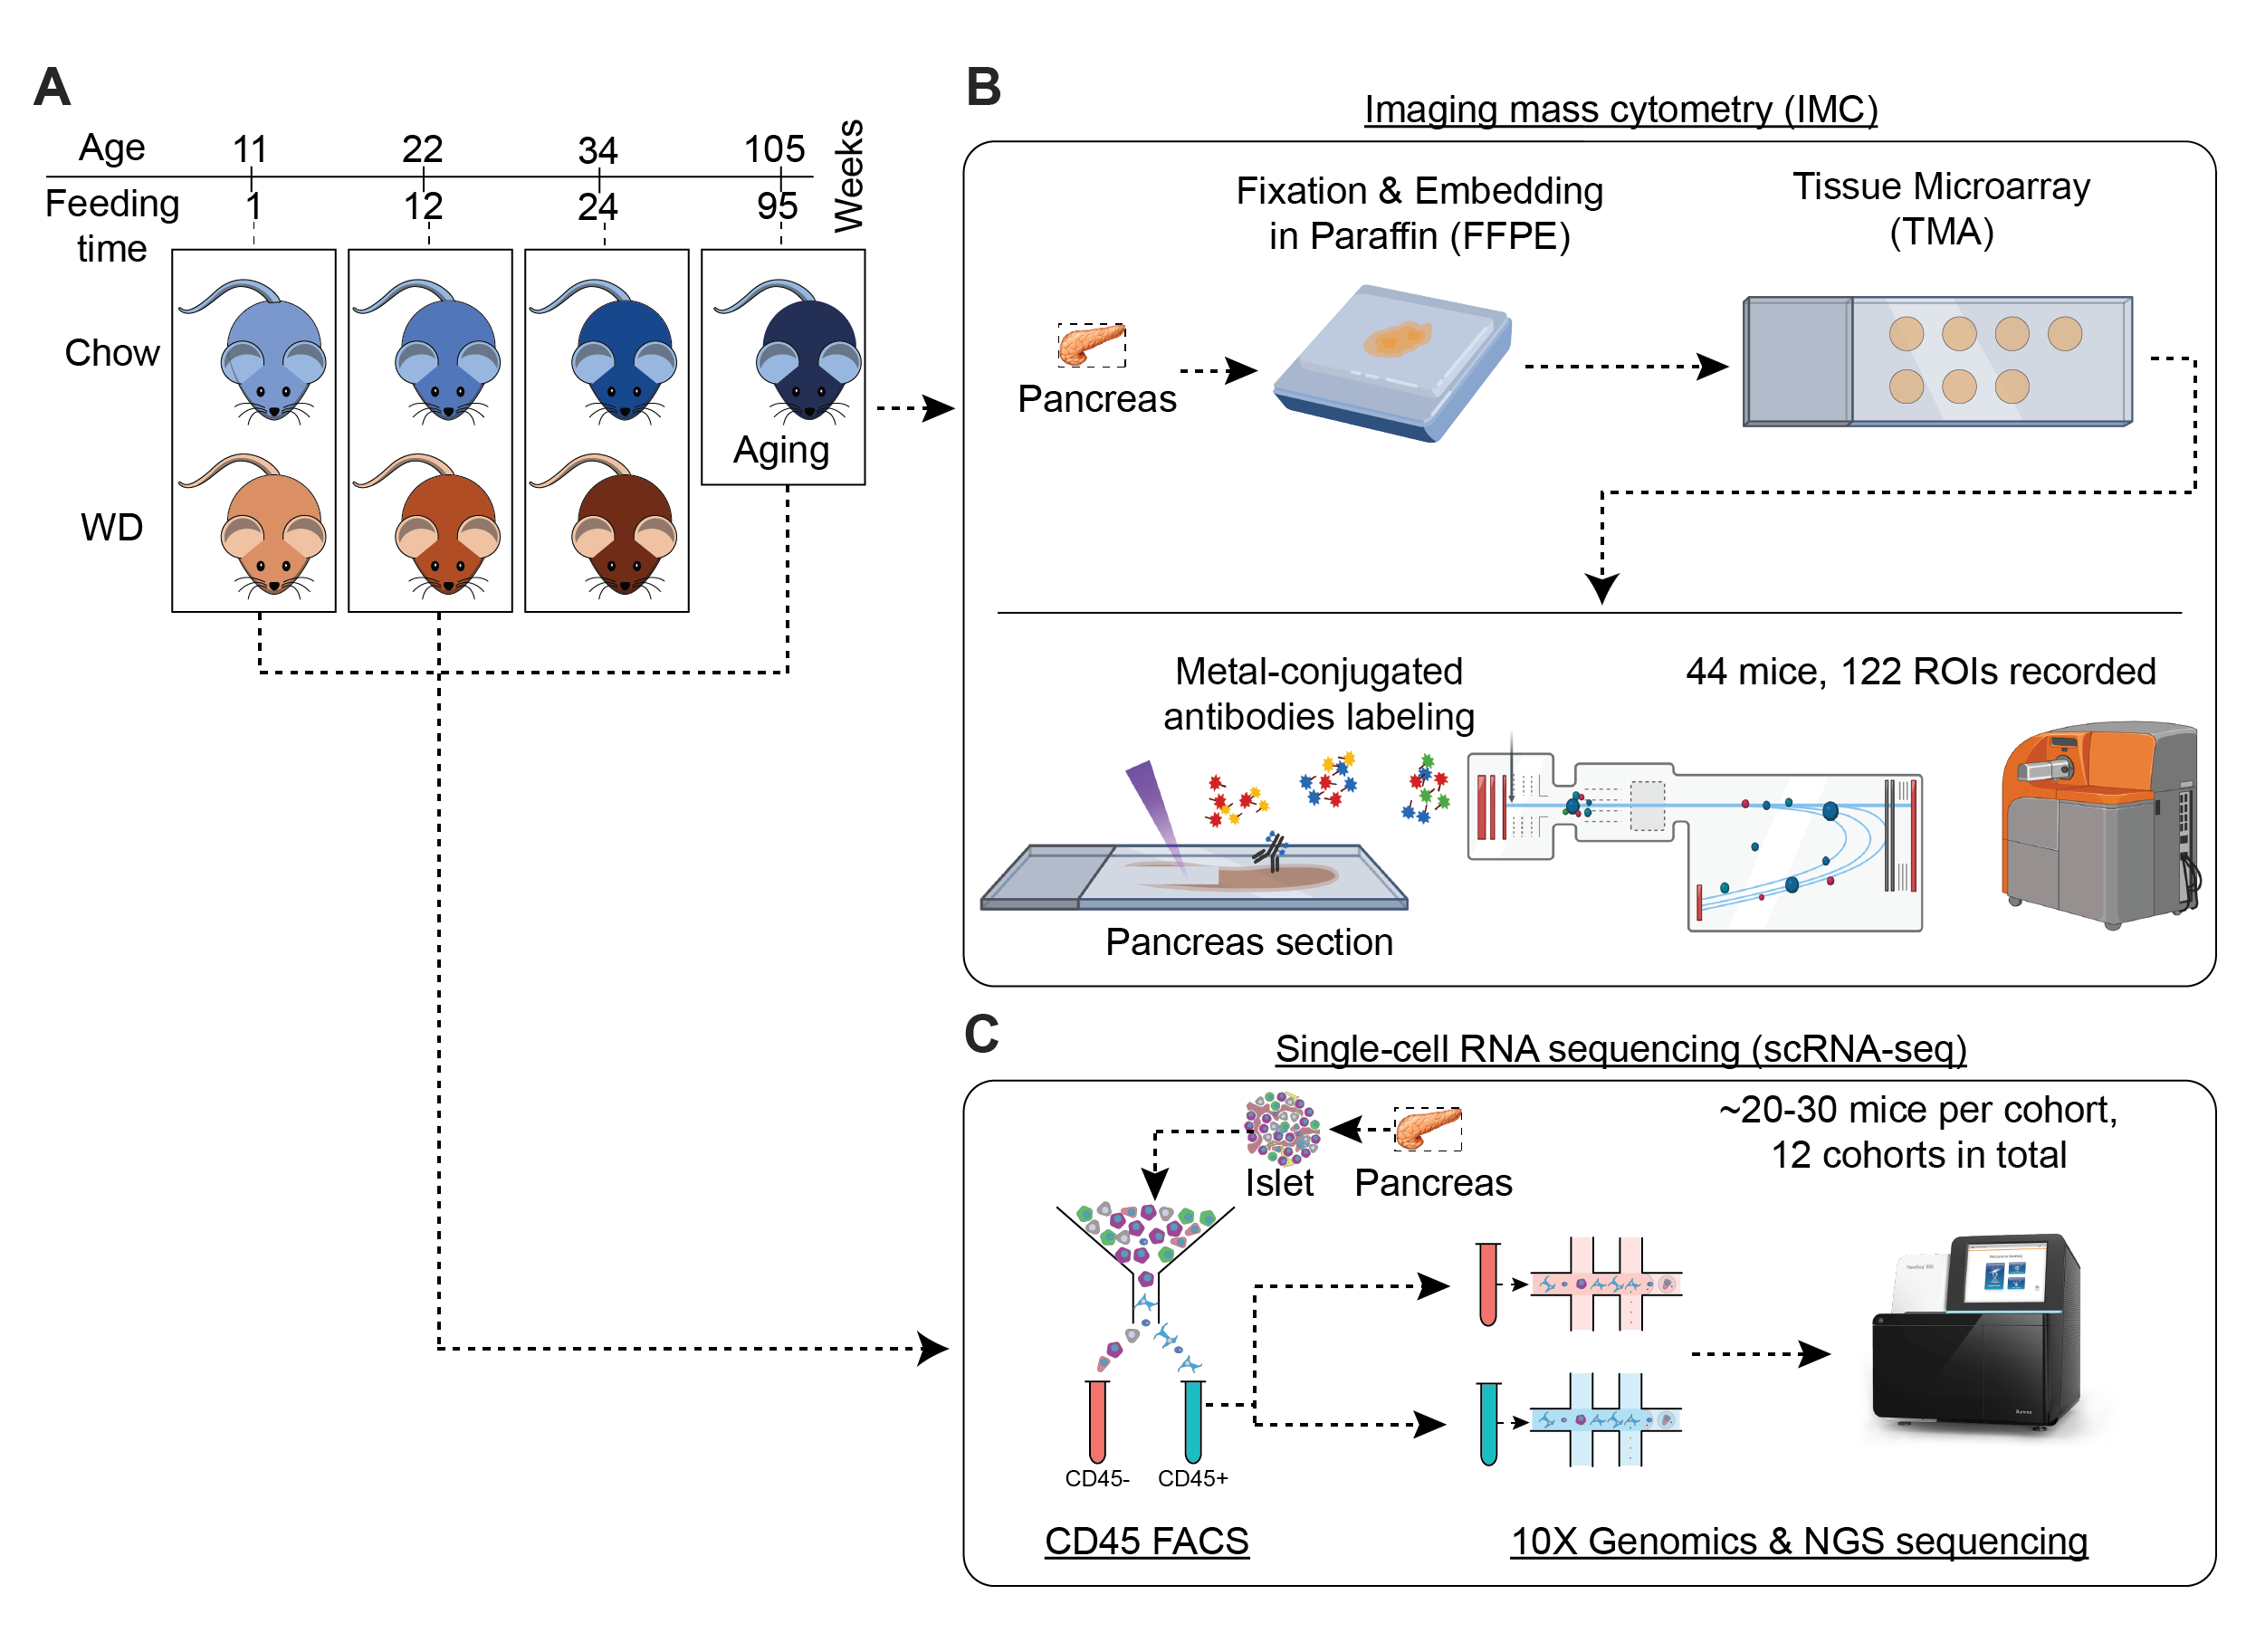
\includegraphics[width=15cm]{Chapter4/Fig/F2-1-01.png}
\caption[Experimental Design]{\textbf{Schematic illustration of experimental design.} This illustration outlines the methodology where pancreas samples were harvested from five mice at three post-Western Diet (WD) intervals (1, 12, and 24 weeks), alongside samples from age-matched, chow-fed mice and 2-year-old aging mice. These samples underwent IMC analysis using an established panel of markers targeting several immune populations, islet β-cells and endothelial cells. For scRNAseq analysis islets from ten cohorts across early (1 week) and mid-term (12 weeks) Western Diet stages, as well as from two aging cohorts, were isolated. Over 20 mice contributed to each cohort. Post-isolation, islet cells were FACS-sorted into immune (CD45\textsuperscript{+}) and non-immune (CD45\textsuperscript{-}) groups and processed via the 10x Genomics v3 protocol, and sequenced.}
\label{fig:wdaging_experimental_design}
\end{figure}

 tissue sections from mice subjected to WD or a control Chow diet feeding for 1 week (W1), 12 weeks (W12), or 24 weeks (W24). In addition, we incorporated samples from an aged cohort (105 weeks old) to contrast between metabolic and aging-associated stress. This allowed us to compare the spatial organization of immune cells under these conditions. To complement the IMC spatial data with molecular profiles, we performed \textbf{single-cell RNA-sequencing (scRNA-seq)} on isolated CD45\textsuperscript{+} immune cells and CD45\textsuperscript{-} non-immune populations from the pancreatic islets obtained from the same mouse cohorts. In the scRNA-seq analysis, our objective was to detect initial molecular alterations triggered by the WD feeding, focusing on samples collected at Week-1 and Week-12 (\textbf{Fig.\ref{fig:wdaging_experimental_design}}).





%\clearpage


\section{Unraveling complex cellular heterogeneity within the\\pancreatic exocrine tissue and within islets}
\subsubsection{IMC Data Analysis}
In the IMC analysis, pancreatic tissue sections from at least 4 mice for each experimental condition and time-point were included. From each section, at least 10 regions of interest (ROIs) were dissected, which were combined to a total of 92 ROIs to create tissue microarrays (TMA), each of which contained ROIs from different experimental conditions and time-points. Overall, a total of 17 TMAs were subjected to comprehensive IMC analysis of 25 selected immune cell marker proteins, markers of pancreatic islets and CD31 in order to identify endothelial cells \textbf{(Table???)}. Using a comprehensive, standardized cell segmentation workflow (\textbf{Fig. \ref{suppl_fig:imc_segmentation}}), we achieved single cell resolution of our IMC analysis. We also included one ROI from a spleen sample in each individual TMA. This served as an anchor reference (see Methods) for the batch correction of all immune cell marker channels across all TMAs (\textbf{Fig.\ref{suppl_fig:imc_anchor}}).\\

\begin{figure}[t]
\centering
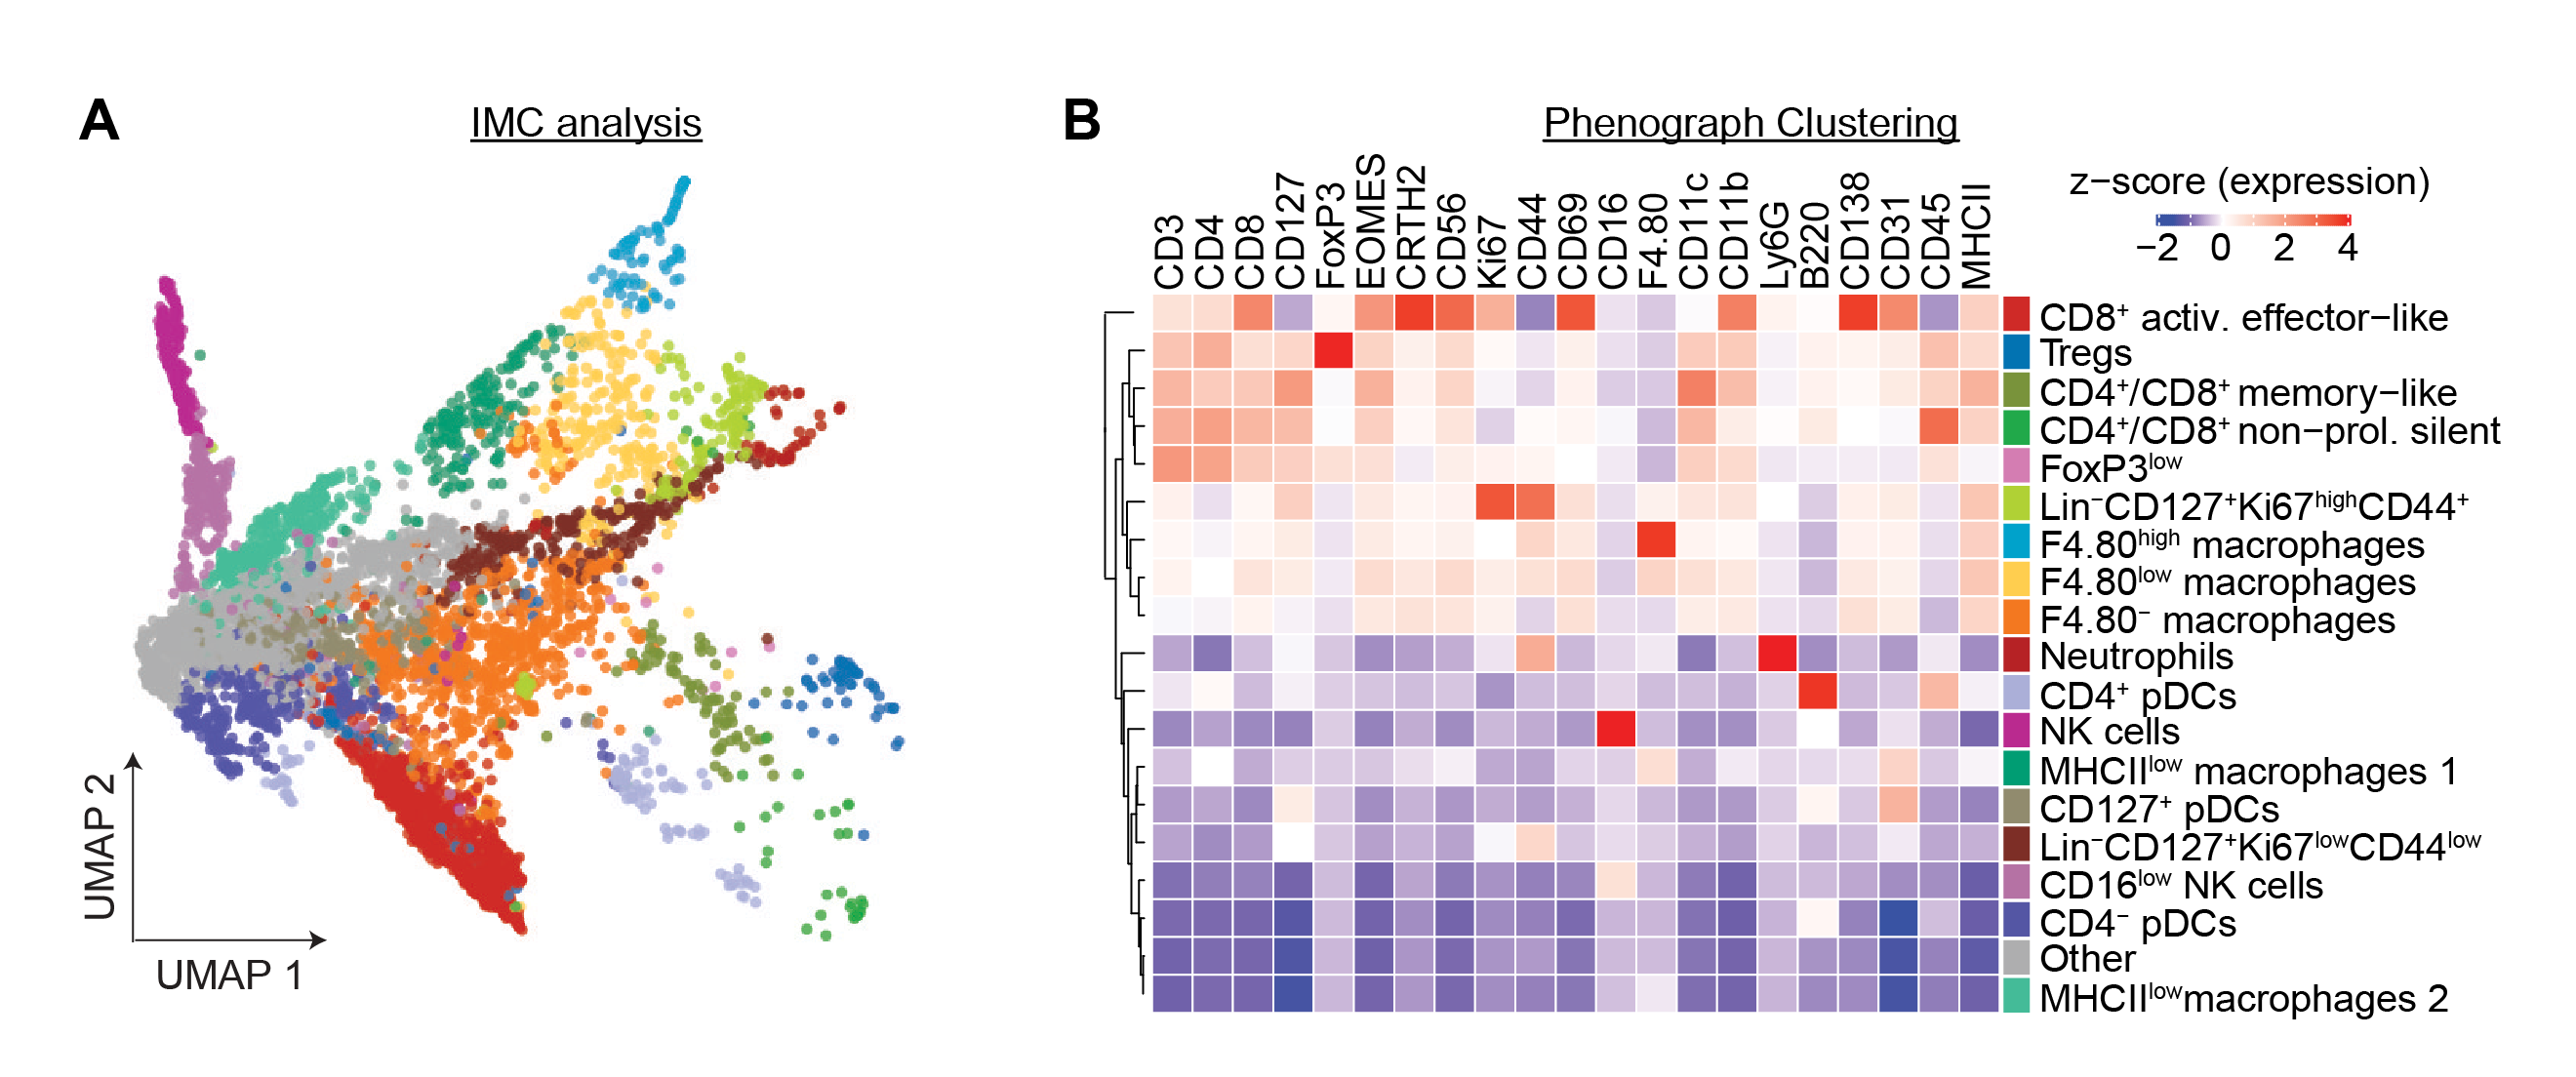
\includegraphics[width=\linewidth]{Chapter4/Fig/F2-2-01.png}
\caption[res-imc]{\textbf{IMC Analysis.} \textbf{(A)} UMAP embedding of the CD45\textsuperscript{+}CD19\textsuperscript{-} immune cell populations identified by IMC analysis. \textbf{(B)}  Heatmap depicting the Phenograph clustering and transformed \textit{z-scores} of protein expression for the immune cell marker channels. The identities of the sub-populations were defined based on the relative expression levels of these marker proteins.}
\label{fig2-2}
\end{figure}

The pancreatic islets were identified using the INS, NKX6-1 and GLP-1 channels, whereas the pancreatic lymph nodes were marked using B220, CD19, CD44 and CD45 channels \textbf{(Table???)}. Interestingly, CD19\textsuperscript{+} B-cells were nearly all localized within the pancreatic lymph nodes (\textbf{Fig.\ref{suppl_fig:imc_bcell}}) and were therefore, not selected for subsequent analyses. Cluster analysis of the selected CD45\textsuperscript{+}CD19\textsuperscript{-} immune cells using Phenograph enabled us to identify a wide variety of immune cell populations, including different CD3 expressing T-cell sub-populations, such as Eomes\textsuperscript{+}CD56\textsuperscript{+}KI67\textsuperscript{+}CD69\textsuperscript{+} activated effector-like CD8\textsuperscript{+} cells, FOXP3\textsuperscript{+} T-regulatory cells, CD127\textsuperscript{\textit{high}}CD4\textsuperscript{+}/CD8\textsuperscript{+} memory-like cells, Ki67\textsuperscript{-}CD4\textsuperscript{+}/CD8\textsuperscript{+} non-proliferative silent cells, and Foxp3\textsuperscript{\textit{low}}CD4\textsuperscript{+} T-cells, differently activated macrophage sub-populations such as F4/80\textsuperscript{-}CD11c\textsuperscript{\textit{high}}, F4/80\textsuperscript{\textit{low}}CD11c\textsuperscript{\textit{high}}, F4/80\textsuperscript{\textit{high}}CD11c\textsuperscript{\textit{high}}, and two MHC-II\textsuperscript{\textit{low}} sub-populations, three types of B220 expressing plasmacytoid dendritic-like cells (CD4\textsuperscript{+}, CD4\textsuperscript{-}, and CD127\textsuperscript{+}), Ly6G\textsuperscript{+} neutrophils, CD16\textsuperscript{\textit{high}} natural killer (NK) cells, and Lin\textsuperscript{-}CD127\textsuperscript{+} innate lymphoid-like cells (ILCs) (\textbf{Fig. \ref{fig2-2} A,B}).\\\\
Our IMC analysis facilitated not only identification and characterization of diverse immune cell populations within the murine pancreatic tissue, but also provided insights into their spatial distribution in relation to WD feeding and aging. 



\subsubsection{scRNA-seq Data Analysis}
Similarly, we applied a robust quality control and data integration pipeline to our scRNA-seq data ( \textbf{Fig. \ref{suppl_fig:sc_qc} A-C}, see \textbf{Methods}), yielding 125,372 high-quality single-cell transcriptomic profiles of CD45\textsuperscript{+} immune cells and CD45\textsuperscript{-} non-immune cells, which were annotated as such, based on the expression of CD45 gene (\textit{Ptprc}) (\textbf{Fig. \ref{fig2-3} A}). The immune and the non-immune populations were further analyzed separately by subsetting the respective cells, performing additional QC steps when necessary and re-integrating the subsets to allow for more granular characterization of the immune and non-immune populations within the pancreatic islets.\\\\
Our approach, focusing on CD45 enrichment  (\textbf{Fig.\ref{fig:wdaging_experimental_design}C}), allowed us to profile a total of 46,913 islet-associated immune cells, which currently represents the most comprehensive immune cell map available for mouse islets (\textbf{Fig.\ref{fig2-3} B}). Utilizing the expression of known markers (\textbf{Fig. \ref{fig2-3} D}), we confirmed the presence of macrophages (marked by \textit{Lyz2, Adgre1, C1qc}), monocytes (identified by \textit{Fn1, Plac8}), neutrophils (evidenced by high \textit{S100a9, S100a8} transcription), dendritic cells (indicated by \textit{Xcr1, Flt3, Siglech}), and a variety of lymphocytes such as T-cells (expressing \textit{Cd3e, Cd4, Cd8a}), B-cells (transcribing \textit{Cd19, Cd79a} and \textit{Cd79b}), and Plasma cells (marked by \textit{Jchain}). The macrophages represented the major immune pop-

\begin{figure}[H]
\centering
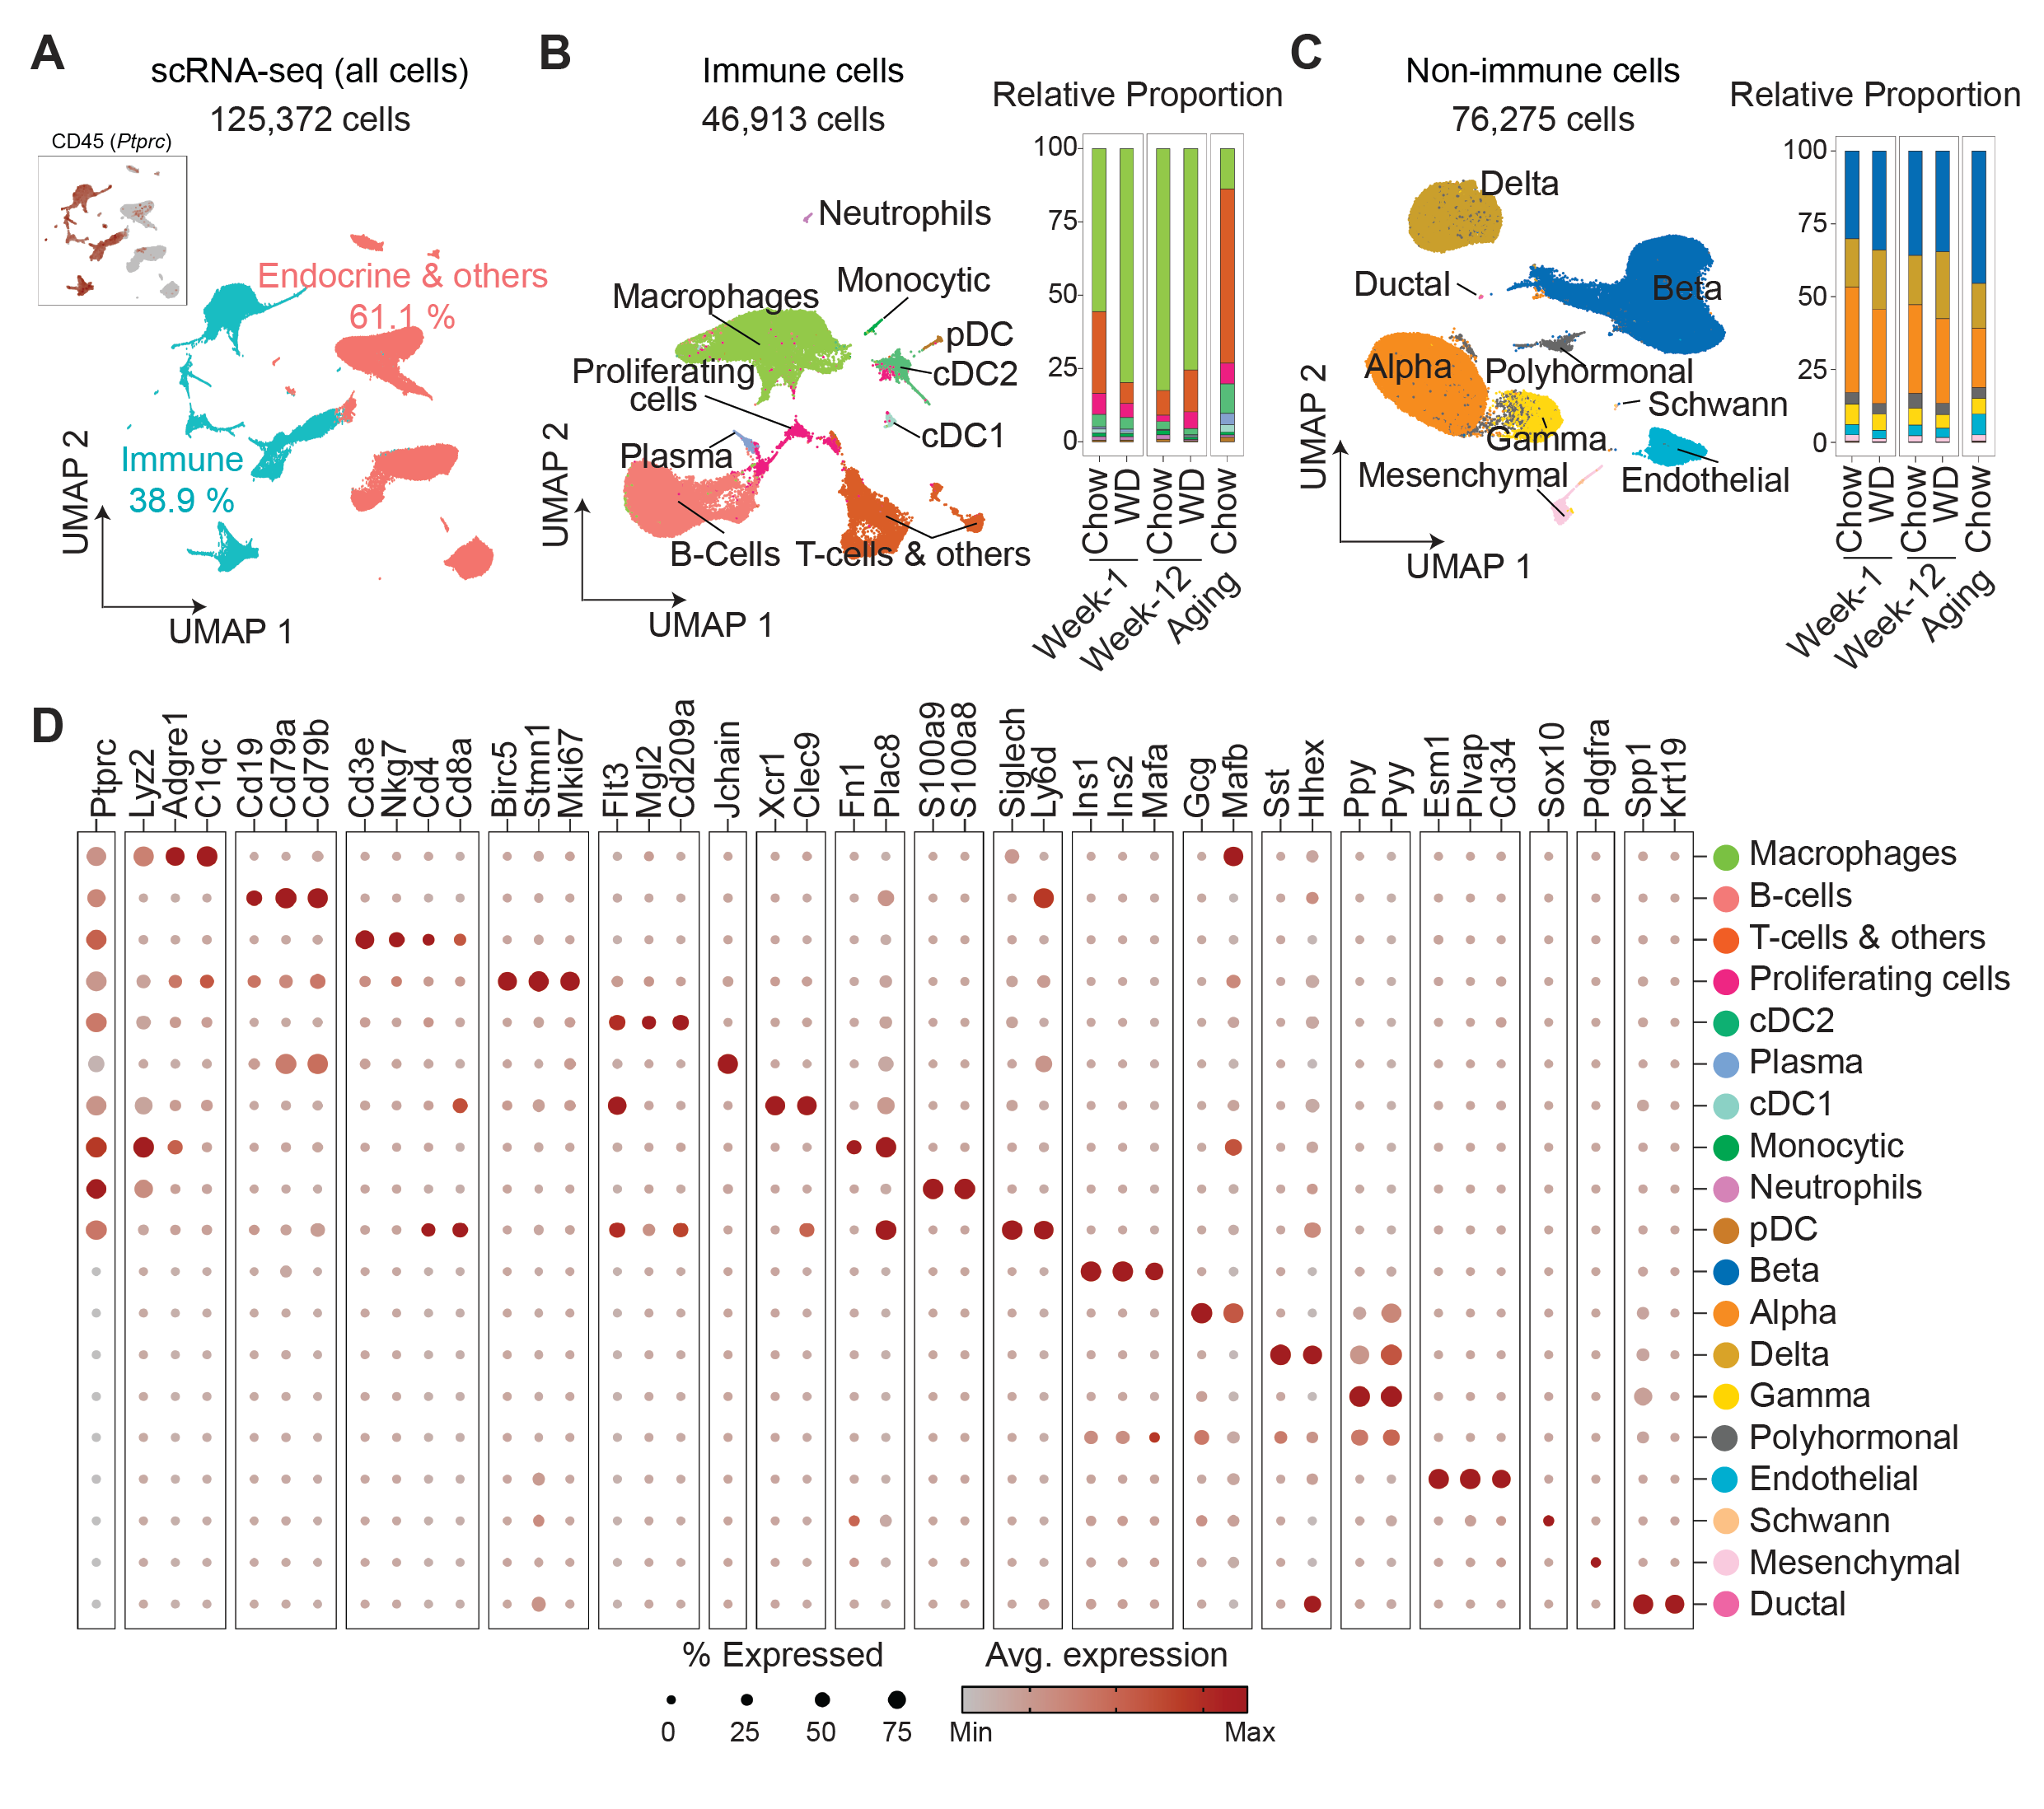
\includegraphics[width=\linewidth]{Chapter4/Fig/F2-3-01.png}
\caption[res-scR]{\textbf{scRNA-seq Analysis.} \textbf{(A)} UMAP embedding of the integrated data consisting of \textit{125,372} single cells across twelve cohorts. The \textbf{‘Immune’} cells were annotated as such based on the expression of CD45 (\textit{Ptprc}) and the remaining cells were labelled as \textbf{‘Endocrine \& others’}. Values indicate the overall proportion of each annotated population. \textbf{(B)} UMAP embedding of the \textbf{‘Immune’} cell population from panel \textbf{(A)}, following sub-setting, additional QC and subsequent re-integration. Cluster identities were defined based on the expression of known immune markers. \textbf{(C)} The proportion of each annotated immune cell sub-populations in panel \textbf{(B)} computed as a percentage of total immune cells in every experimental group. The cells from different biological replicate cohorts were pooled together. B-cells were excluded from calculation and therefore not represented in the bar-plot. \textbf{(D)} UMAP embedding of the \textbf{‘Endocrine \& others’} cell populations from panel \textbf{(A)}, following sub-setting, additional QC and subsequent re-integration. Cluster identities were defined based on the expression of known gene markers. \textbf{(E)} The proportion of each annotated endocrine, exocrine and other cell populations in panel \textbf{(D)} computed as a percentage of total non-immune cells in every experimental group. The cells from different biological replicate cohorts were pooled together. \textbf{(F)} Combined dot-plot showing hallmark  marker genes for all annotated cell-types in panels \textbf{(B)} and \textbf{(D)}.}
\label{fig:chp2_fullscRNA}
\end{figure}


 -ulation within the islets of non-aging Chow and WD-fed cohorts (W1 and W12). However, the proportion of T-cells was the highest in the chow-fed aging cohort which is in line with the observation of significant accumulation of T-cells in aging mice. Of note, B-lymphocytes were also excluded in downstream analyses of the scRNA-seq data, as they were primarily associated with pancreatic lymph nodes in the IMC analysis (\textbf{Fig.\ref{suppl_fig:imc_anchorbcell} B,C}) and their proportion across the single-cell cohorts was also inconsistent (\textbf{Fig.\ref{suppl_fig:sc_qc} A}). The remaining immune populations represented a minor fraction of the total islet-associated immune cells across all cohorts in the single-cell data (\textbf{Fig.\ref{fig2-3} B, Relative Proportion}). Our scRNA-seq analysis further enabled the investigation of islet-associated immune cells at a resolution that is significantly superior to that achievable with immunohistochemistry (IHC).\\


In addition to the immune cells, we also profiled 76,275 islet-associated CD45\textsuperscript{-} cells from the same cohort of animals, which consisted of pancreatic Endocrine and Exocrine cells, Endothelial cells, Mesenchymal cells and Schwann cells, based on well-established hallmark gene expression patterns (\textbf{Fig. \ref{fig2-3} C-D, Fig.\ref{suppl_fig:sc_qc} B}). We annotated the endocrine populations as Alpha \textbf{α} (\textit{Gcg, Mafb}), Beta \textbf{β} (\textit{Ins1, Ins2, Mafa}), Gamma \textbf{γ} (\textit{Ppy, Pyy}), also known as pancreatic polypeptide (PP) and Delta \textbf{δ} (\textit{Sst, Hhex}) cells based on the expression of primary islet hormones and TFs (\textbf{Fig. \ref{fig2-3} C-D}). β-cells constituted the major fraction of endocrine cells (~37\%), followed by α-cells (~30\%), δ-cells (~19\%) and PP-cells (~6\%). Consistent with methodologies employed in published reports, endocrine cells expressing more than one hormone marker were classified as Polyhormonal cells and accounted for ~4\% of the data (\textbf{Fig.\ref{suppl_fig:sc_qc} D,E}). These mixed population were omitted from further analysis. In line with previous studies, the proportion of β-cells in the chow diet fed aging cohort was higher compared to the all the non-aging cohorts (\textbf{Fig.\ref{fig2-3} C, Relative Proportion}). The other endocrine populations, as well as the exocrine cells, did not show any shifts in their cellular proportions in response to metabolic stress or aging. The Mesenchymal (2\%), Schwann (1\%), Ductal (1\%) and Endocthelial (5\%) cells together made up less that 10\% of the single-cell data, thereby reflecting the efficiency of the islet isolation step during sample preparation. 

%\clearpage

\section{Metabolic stress accelerates aging-induced accumulation of\\inflammatory F4/80\textsuperscript{\textit{low}} macrophages within the pancreas}
\label{sec:imc_acceleration}

We subsequently investigated whether immune cell populations within the pancreas expanded in response to overnutrition induced by WD-feeding and aging. Using IMC, we assessed the density of each immune cell population and detected major changes in the macrophage compartment across metabolic stress and aging (\textbf{Table. \ref{TAB}}). This mainly affected the three macrophage sub-populations expressing medium to high MHCII levels: F4/80\textsuperscript{\textit{high}}, F4/80\textsuperscript{\textit{low}}, and F4/80\textsuperscript{\textit{-}} (\textbf{Fig. \ref{fig2-9} A}). Our analysis primarily centered on two major aspects of sub-population dynamics: 
\begin{enumerate}
    \item The relative enrichment of these cells within the entire pancreas and
    \item The accumulation of these immune cells in specific regions, namely the pancreatic islets and the peri-islet areas.
\end{enumerate}

\begin{figure}[t!]
    \centering
    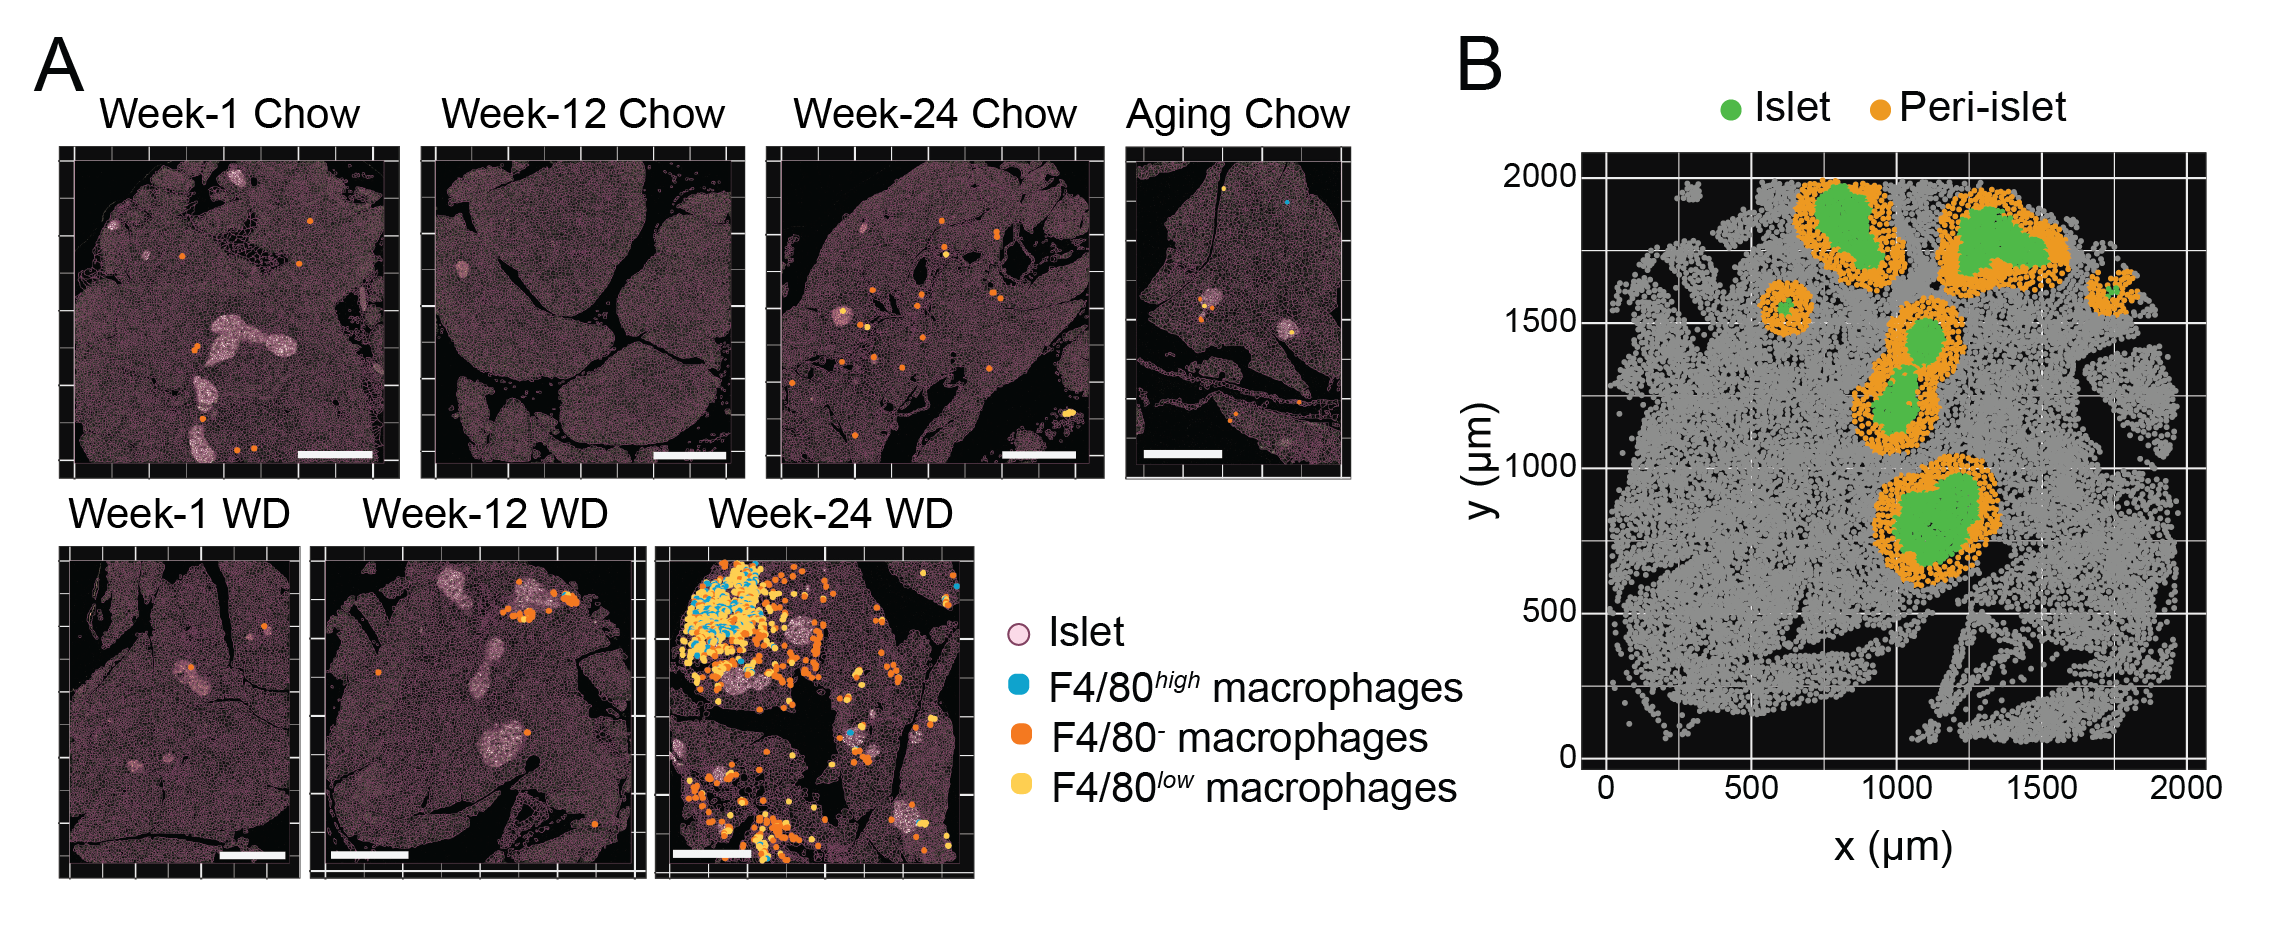
\includegraphics[width=\linewidth]{Chapter4/Fig/F2-9-01.png}
    \caption[res-imc2]{\textbf{Metabolic stress accelerates aging-induced accumulation of inflammatory F4/80\textsuperscript{\textit{low}} macrophages within the pancreas.} \textbf{(A)} Representative ROIs showing the three macrophage sub-populations expressing medium to high MHCII levels: F4/80\textsuperscript{\textit{high}}, F4/80\textsuperscript{\textit{low}}, and F4/80\textsuperscript{\textit{-}} in the pancreas. Pancreatic islet regions are marked by raw insulin (INS) signal. Scale bar 500 μm. \textbf{(B)} Representative image illustrating a pancreatic islet (green) enclosed by peri-islet region (yellow) encompassing the area extending from the islet boundary up to 70 μm away. \textbf{(C)} Scatter plots showing the density of F4/80\textsuperscript{\textit{high}} (left), F4/80\textsuperscript{\textit{low}} (middle) and F4/80\textsuperscript{\textit{-}} (right) macrophages in the pancreas across four time points and two feeding conditions. Linear regression fits representing the cell density trends over time are plotted as solid lines. The 95\% confidence intervals for each linear regression are highlighted in grey. Each condition includes data from n $\geq$ 3 mice. p-values for regressions were determined using t-tests. \textbf{(D)} Scatter plots showing the density of F4/80\textsuperscript{\textit{high}} (left), F4/80\textsuperscript{\textit{low}} (middle) and F4/80\textsuperscript{\textit{-}} (right) macrophages in the pancreatic islet and peri-islet regions across four time points and two feeding conditions. Linear regression fits representing the cell density trends over time are plotted as solid lines. The 95\% confidence intervals for each linear regression are highlighted in grey. Each condition includes data from n $\geq$ 3 mice. p-values for regressions were determined using t-tests.}
    \label{fig2-9}
\end{figure}

To address the second aspect, we identified the islet regions based on the expression of insulin (INS) channel. To evaluate both, the expansion of islet-resident immune cells and the recruitment of immune cells to the periphery of the islet, we expanded our analysis to include the peri-islet region, by extending 70μm beyond the boundary of the INS+ islets (\textbf{Fig. \ref{fig2-9} B}). Our observations indicated that while most immune cell populations in the pancreas remained stable under metabolic stress or progressive aging (\textbf{Fig.\ref{fig2-9} C, Fig.\ref{suppl_fig:imc_peri}}), there was a notable rise in F4/80\textsuperscript{\textit{low}} macrophages (\textbf{Fig. \ref{fig2-9} C middle, Fig.\ref{suppl_fig:imc_peri} B,E}). These cells also accumulated within the islets and their adjacent areas (\textbf{Fig. \ref{fig2-9} D, middle}). Overnutrition also caused a mild elevation in F4/80\textsuperscript{\textit{-}} macrophages throughout the pancreas (\textbf{Fig.\ref{fig2-9} C right, Fig.\ref{suppl_fig:imc_peri} B,E}), whereas F4/80\textsuperscript{\textit{high}} macrophages remained relatively steady, irrespective of conditions (\textbf{Fig. \ref{fig2-9} C left,Fig.\ref{suppl_fig:imc_peri} B,E}). Moreover, F4/80\textsuperscript{\textit{high}} (\textbf{Fig.\ref{fig2-9} D left})  and F4/80\textsuperscript{\textit{-}} (\textbf{Fig.\ref{fig2-9} D right}) macrophages do not get closer to the islet region under both stress conditions.\\

%\clearpage

In essence, our analysis revealed a WD-mediated acceleration of the accumulation of the F4/80\textsuperscript{\textit{low}} macrophage population within the pancreas and peri-islet regions, which under Chow diet only happens later in life. Metabolic stress also favored accumulation of another inflammatory CD11c\textsuperscript{\textit{high}} expressing F4/80\textsuperscript{\textit{-}} macrophage sub-population, which was not observed in aging.  

%\clearpage

\section{Interferon-activated macrophages are enriched in the islets\\in response to metabolic- and aging-induced stress.}
\label{sec:sc_macs}

Macrophages are the only resident myeloid cells found in islets of all mouse strains, under normal conditions \textbf{\cite{zakharov_single-cell_2020}}. The presence of islet-resident macrophages is essential for the normal islet development, β-cell regeneration and regulation of insulin secretion \textbf{\cite{ying_expansion_2019}}. In diet-induced islet inflammation, islet-resident macrophages have been shown to impair β-cell insulin secretion while also promoting adaptive β-cell proliferation via PDGFR signaling. This suggests that macrophages within islets are heterogeneous in function and that diet could alter the abundance of specific macrophage subsets in pancreatic islets.

%\subsection{Characterization of islet-intrinsic macrophage sub-populations\\using scRNA-seq\\}

\subsubsection{Annotating islet-intrinsic macrophages using gene expression}
To molecularly characterize the islet-associated macrophages, we extracted the macrophages from our single-cell dataset and conducted sub-clustering. We identified a total of five macrophage sub-populations which included a homeostatic (non-activated) population (\textbf{Macs-1}), two activated populations (\textbf{Macs-2} and \textbf{Macs-3}), a proliferating population (\textbf{Macs-4}), and a phagocytic population (\textbf{Macs-5}) (\textbf{Fig. \ref{fig2-5-1} A}). Contrary to the homeostatic Macs-1, both

\begin{figure}[H]
\centering
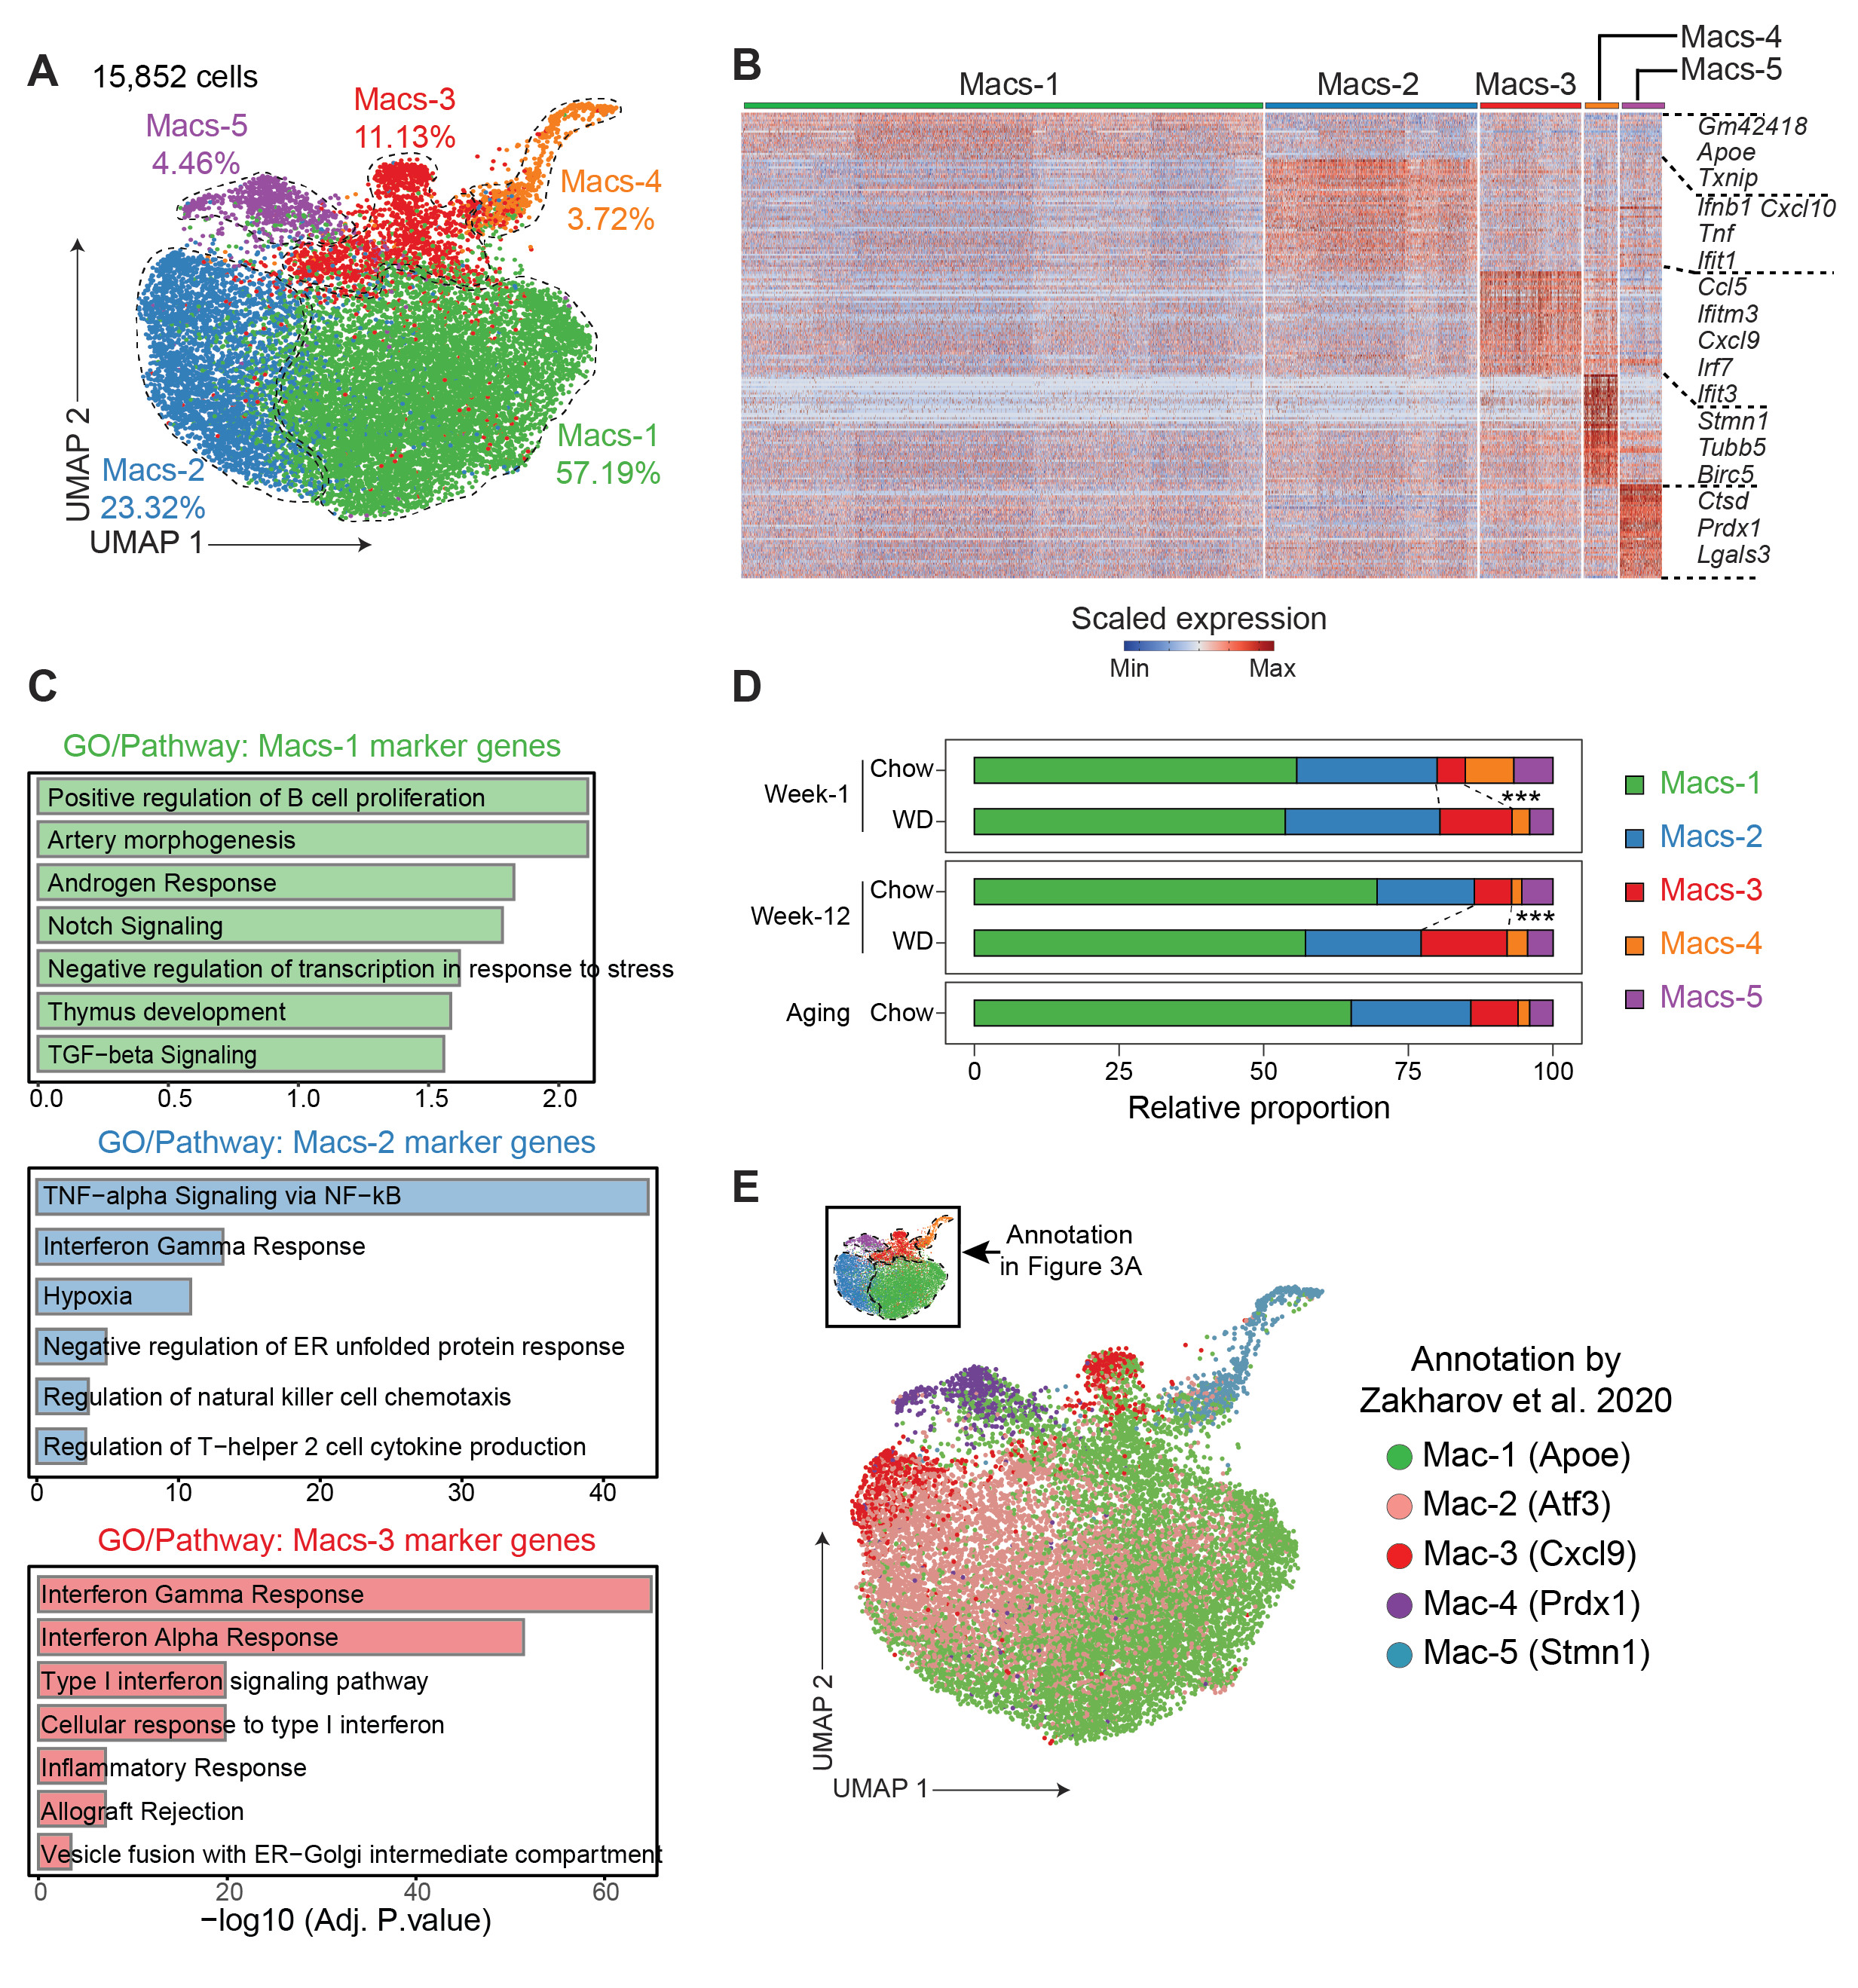
\includegraphics[width=\linewidth]{Chapter4/Fig/F2-5-01.png}
\caption[res-macs1]{\textbf{Characterization of islet-intrinsic macrophage sub-populations using scRNA-seq.}\\
\textbf{(A)} UMAP embedding of pancreatic islet associated macrophages, pooled from various time-points (Week-1, Week-12, and Aging) and dietary conditions (WD and Chow). Values indicate the overall proportion of each defined subtype. The identities of sub-populations were defined based on marker gene expression. \textbf{(B)} Heatmaps showing scaled expression levels of marker genes in each macrophage subpopulation from panel (A). \textbf{(C)} Enriched GO terms using top markers for the five macrophage sub-populations. Significance (-log10 adjusted p-value) of the enrichments are shown in bar plots.}
\label{fig2-5-1}
\end{figure}


 Macs-2 and Macs-3 displayed a pro-inflammatory phenotype and  a type 2 and 1 interferon response gene signature, respectively (\textbf{Fig. \ref{fig2-5-1} B-C}). The level of activation was more dramatic in Macs-3 than in Macs-2. Intriguingly, the highest expression of \textit{Ifnb1} was observed in Macs-2, suggesting it as the likely initiator of the interferon response (\textbf{Fig. \ref{fig2-5-1} B-C}). Additionally, Macs-2 showed increased expression of genes downstream of Tumor Necrosis Factors (\textit{Tnf}) and \textit{NFκB} when compared to Macs-1, a trait that was not present in Macs-3 (\textbf{Fig. \ref{fig2-5-1} C}). Macs-4 represents group of islet-macrophages expressing genes involved in cell-cycle, and together with Macs-1, likely constitute the macrophages involved in islet functions. Finally, the gene expression signature of Macs-5 was associated with apoptotic cell clearance and strong anti-inflammatory function marked by the expression of \textit{Prdx1} and \textit{Lgals3}.
\clearpage



\begin{wrapfigure}{r}{0.5\textwidth}
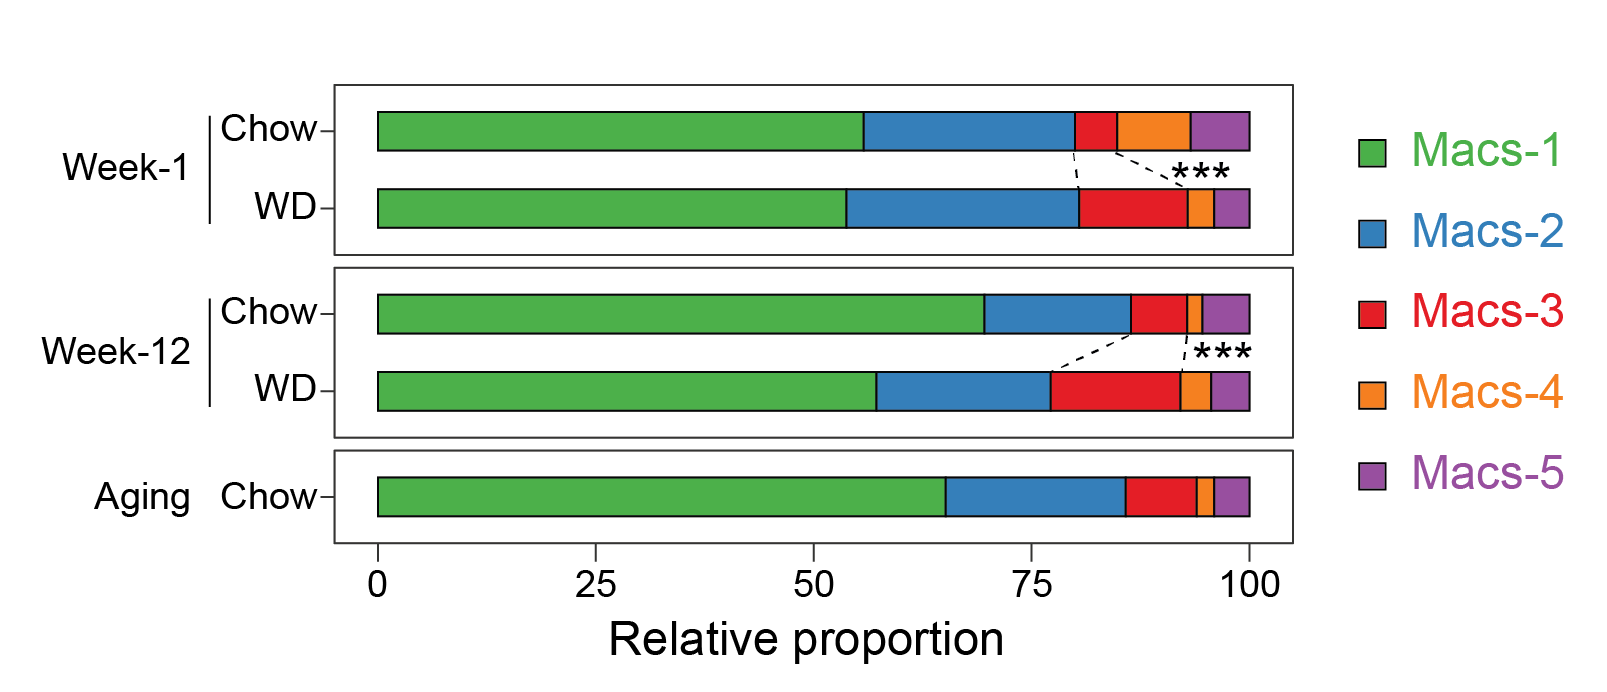
\includegraphics[width=8cm]{Chapter4/Fig/F2-5-03.png}
\caption[res-macs2]{\textbf{Relative proportions of islet macrophages across WD-feeding and aging}. Proportion of each macrophage sub-population in (\textbf{Fig. \ref{fig2-5-1} A}), computed as a percentage of total macrophage cells in every experimental group. The cells from different biological replicate cohorts were pooled together. *: p<0.05, **: p<0.01, ***: p<0.001. p values were calculated from a mixed-effects binomial model.  }
\label{fig:chp2_macs_composition}
\end{wrapfigure}

The proportion of the non-inflammatory Macs-1 was the highest among all islet macrophage sub-populations, with over 50\% of the cells identified as Macs-1 in all conditions. However, there was a rapid and significant expansion of the Macs-3 sub-population in response to WD feeding, and a comparable, albeit less obvious, increase during aging. The This mirrors the stress-induced accumulation of F4.80-low macrophages not just in the pancreas, but also in the islets and the peri-islet region (Figure 2E,I). Compared to Macs-3, the composition of other annotated macrophage sub-populations in the single-cell data, were stable and did not show any changes in response to WD feeding or aging (\textbf{Fig. \ref{fig2-5-2}}).

%\clearpage


\subsubsection{Mapping islet-macrophages from NOD mice}

% \begin{wrapfigure}{l}{0.5\textwidth}
% 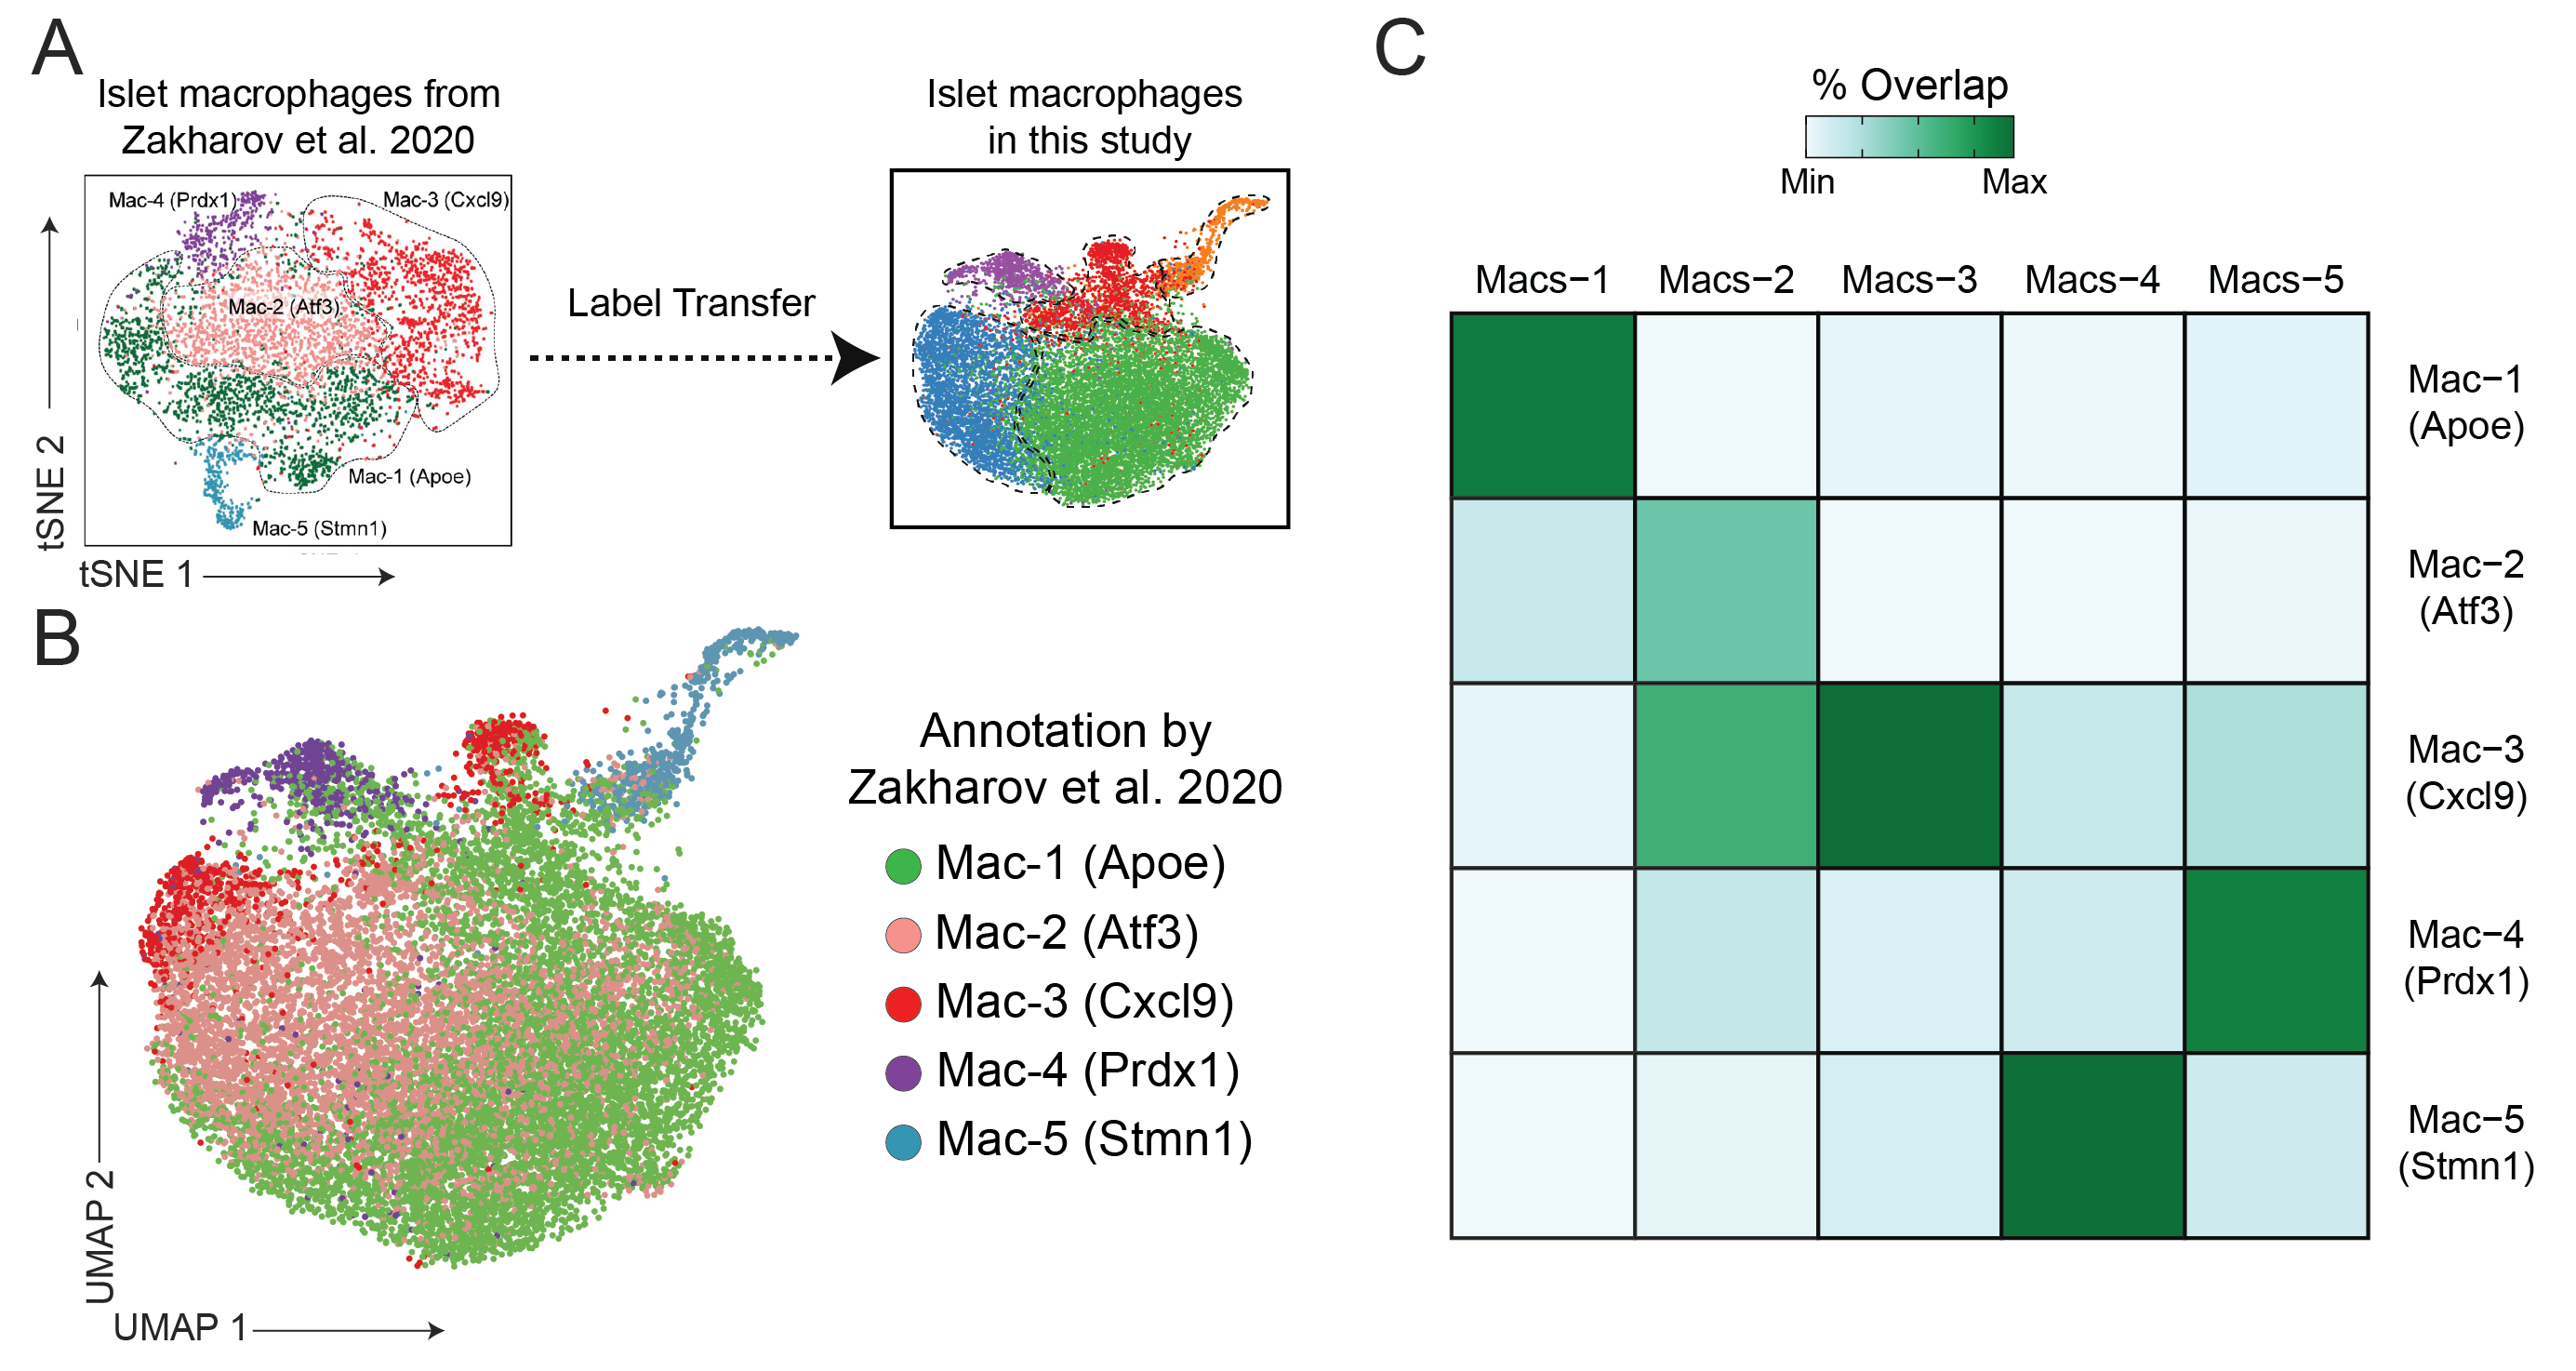
\includegraphics[width=8cm]{Chapter4/Fig/F2-5-02.png}
% \caption[res-macs3]{\textbf{Label transfer of annotations from Zakharov et. al}}
% \label{fig2-5-3}
% \end{wrapfigure}

A similar single-cell study of islet macrophages in NOD mice also identified five main macrophage sub-populations. In the study, the authors identified a non-inflammatory sub-population, \textbf{Mac-1 (\textit{Apoe})}, characterized by elevated levels of \textit{Apoe} and \textit{Trem2}. They also identified two groups of inflammatory activated macrophages, \textbf{Mac-2 (\textit{Atf3})}, characterized by strong \textit{NFκB} activation and elevated expression of genes encoding inflammatory cytokines, and, \textbf{Mac-3 (\textit{Cxcl9})}, which depicted elevated expression of genes encoding several cytokines, costimulatory molecules , and molecules involved in antigen presentation, alongside \textit{NFκB} signature. Additionally, Mac-3 was the only sub-population to show continuous strong expansion during T1D progression. Apart from these three groups, the authors also identified \textbf{Mac-4 (\textit{Prdx1})}, associated with lysosomal activity and apoptotic cell clearance and \textbf{Mac-5 (\textit{Stmn1})}, associated with the cell-cycle pathway (\textbf{Fig. \ref{fig2-5-3}, top left}) \textbf{\cite{zakharov_single-cell_2020}}.  \\

Therefore, noting the transcriptomic similarities between the islet-intrinsic macrophages in T1DM NOD mice and T2DM WD-fed mice, we performed label transfer and mapped these NOD-mice macrophage sub-populations onto our analysis. This analysis revealed a strong correspondence in the islet-resident macrophage sub-populations in the two studies (\textbf{Fig. \ref{fig2-5-3}, bottom}). <ADD MORE SENTENCES>



\subsubsection{Linking macrophage sub-populations from scRNA-seq to IMC}

To establish a link between these macrophage sub-populations and those determined through the IMC analysis, we projected the channels utilized for macrophage categorization in the IMC analysis (Figure 1E) onto the scRNA-seq data. Our investigation indicated that F4/80 expression was highest in Macs-1, reduced in Macs-3, and lowest in Macs-2 (\textbf{Fig. \ref{fig2-4} A, top}). 

\begin{figure}[H]
\centering
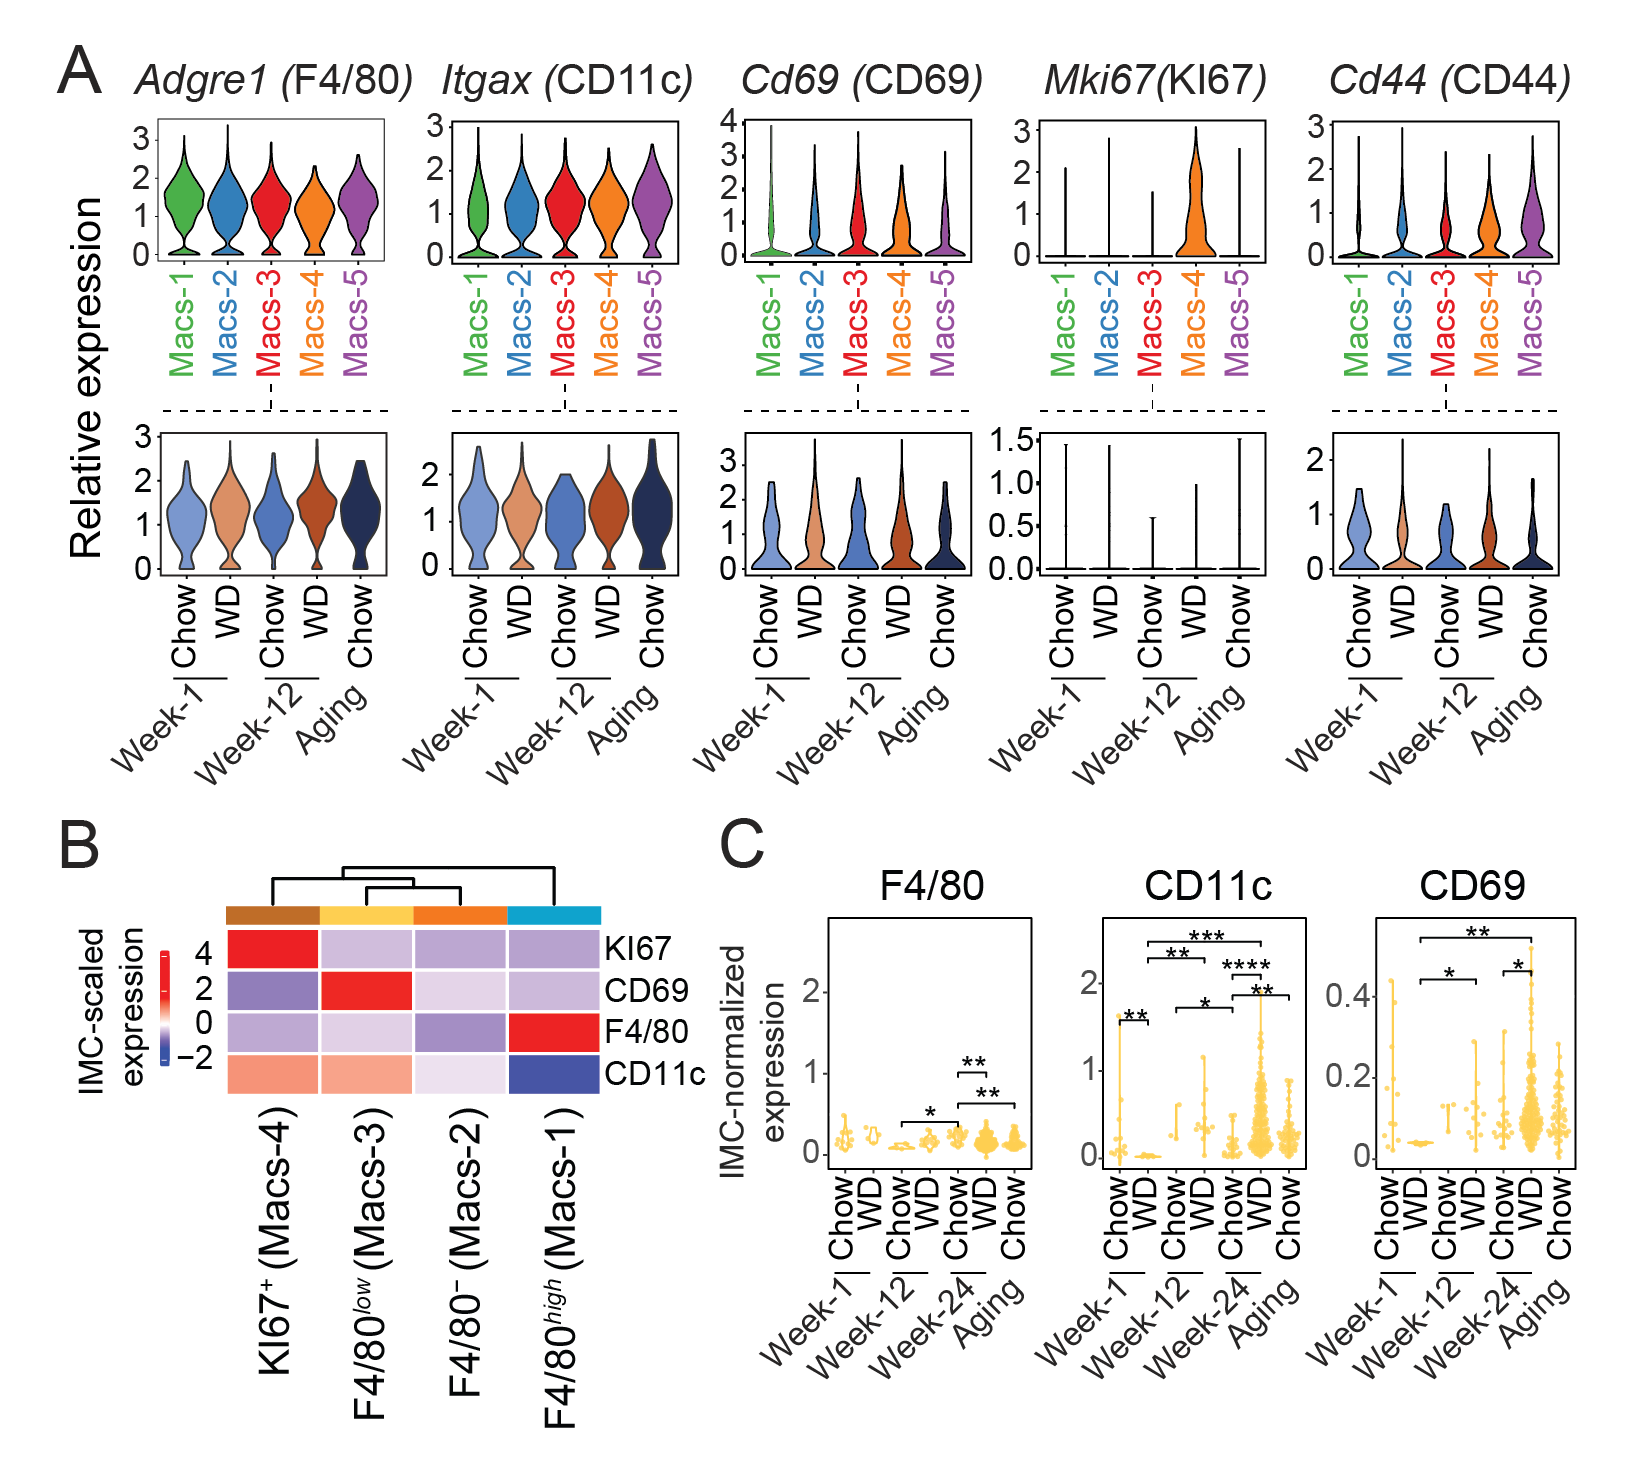
\includegraphics[width=\linewidth]{Chapter4/Fig/F2-4-01.png}
\caption[res-macs2]{\textbf{Linking macrophage sub-populations from scRNA-seq to IMC.} \textbf{(A)} Violin plots depicting the normalized expression levels of genes with corresponding channels in the IMC panel. The top plots compare these levels across various macrophage sub-populations, and the bottom plots display their expression in the Macs-3 population under different experimental conditions. \textbf{(B)}Heatmap showing z-scored expression of selected IMC channgels across the four macrophage sub-populations identified in the IMC analysis. Corresponding macrophage sub-populations from scRNA-seq analysis are indicated in parantheses. \textbf{(C)} Violin plots of \textit{arcsinh} transformed expression of selected IMC channels in the F4/80\textsuperscript{\textit{low}} macrophage sub-population from the IMC analysis across experimental conditions. *p<0.05, **p<0.01, ***p<0.001 and ****p<0.0001. p-values were calculated using the Wilcoxon rank-sum test with Bonferroni correction.} 
\label{fig2-4}
\end{figure}


Observing a similar pattern in the IMC analysis, it was discovered that Macs-1, Macs-2, and Macs-3 correspond to the F4/80\textsuperscript{\textit{high}}, F4/80\textsuperscript{\textit{negative}}, and F4/80\textsuperscript{\textit{low}} sub-populations, respectively. Specifically, Macs-3, akin to the F4/80\textsuperscript{\textit{low}} sub-population, showed moderate F4/80 gene (\textit{Adgre1}) expression but exhibited the highest levels of CD11c (\textit{Itgax}) and CD69 (\textit{Cd69}) transcription as signs of activation (\textbf{Fig. \ref{fig2-4} B}). Moreover, the proliferative Macs-4 population likely equates to the Ki67\textsuperscript{\textit{high}} macrophages observed in the IMC analysis. We did not find an equivalent for the Macs-5 cells in the preceding IMC analysis, suggesting possible discrepancies between protein-based and RNA-based methodologies for cell type annotation.\\



% \mysidecaption{0.4}{%
% \captionof{figure}{\textbf{Linking macrophage sub-populations between scRNA-seq and IMC analyses.} \textbf{(A)} Violin plots depicting the normalized expression levels of selected markers with corresponding channels in the IMC panel. The top plots compare these levels across various macrophage sub-populations, and the bottom plots display their expression in the Macs-3 population under different experimental conditions. \textbf{(B)}Heatmap showing z-scored expression of selected IMC channgels across the four macrophage sub-populations identified in the IMC analysis. Corresponding macrophage sub-populations from scRNA-seq analysis are indicated in parantheses. \textbf{(C)} Violin plots of \textit{arcsinh} transformed expression of selected IMC channels in the F4/80\textsuperscript{\textit{low}} macrophage sub-population from the IMC analysis across experimental conditions. * p<0.05, ** p<0.01, *** p<0.001 and **** p<0.0001. p-values were calculated using the Wilcoxon rank-sum test with Bonferroni correction.}%
% }
% {%
% 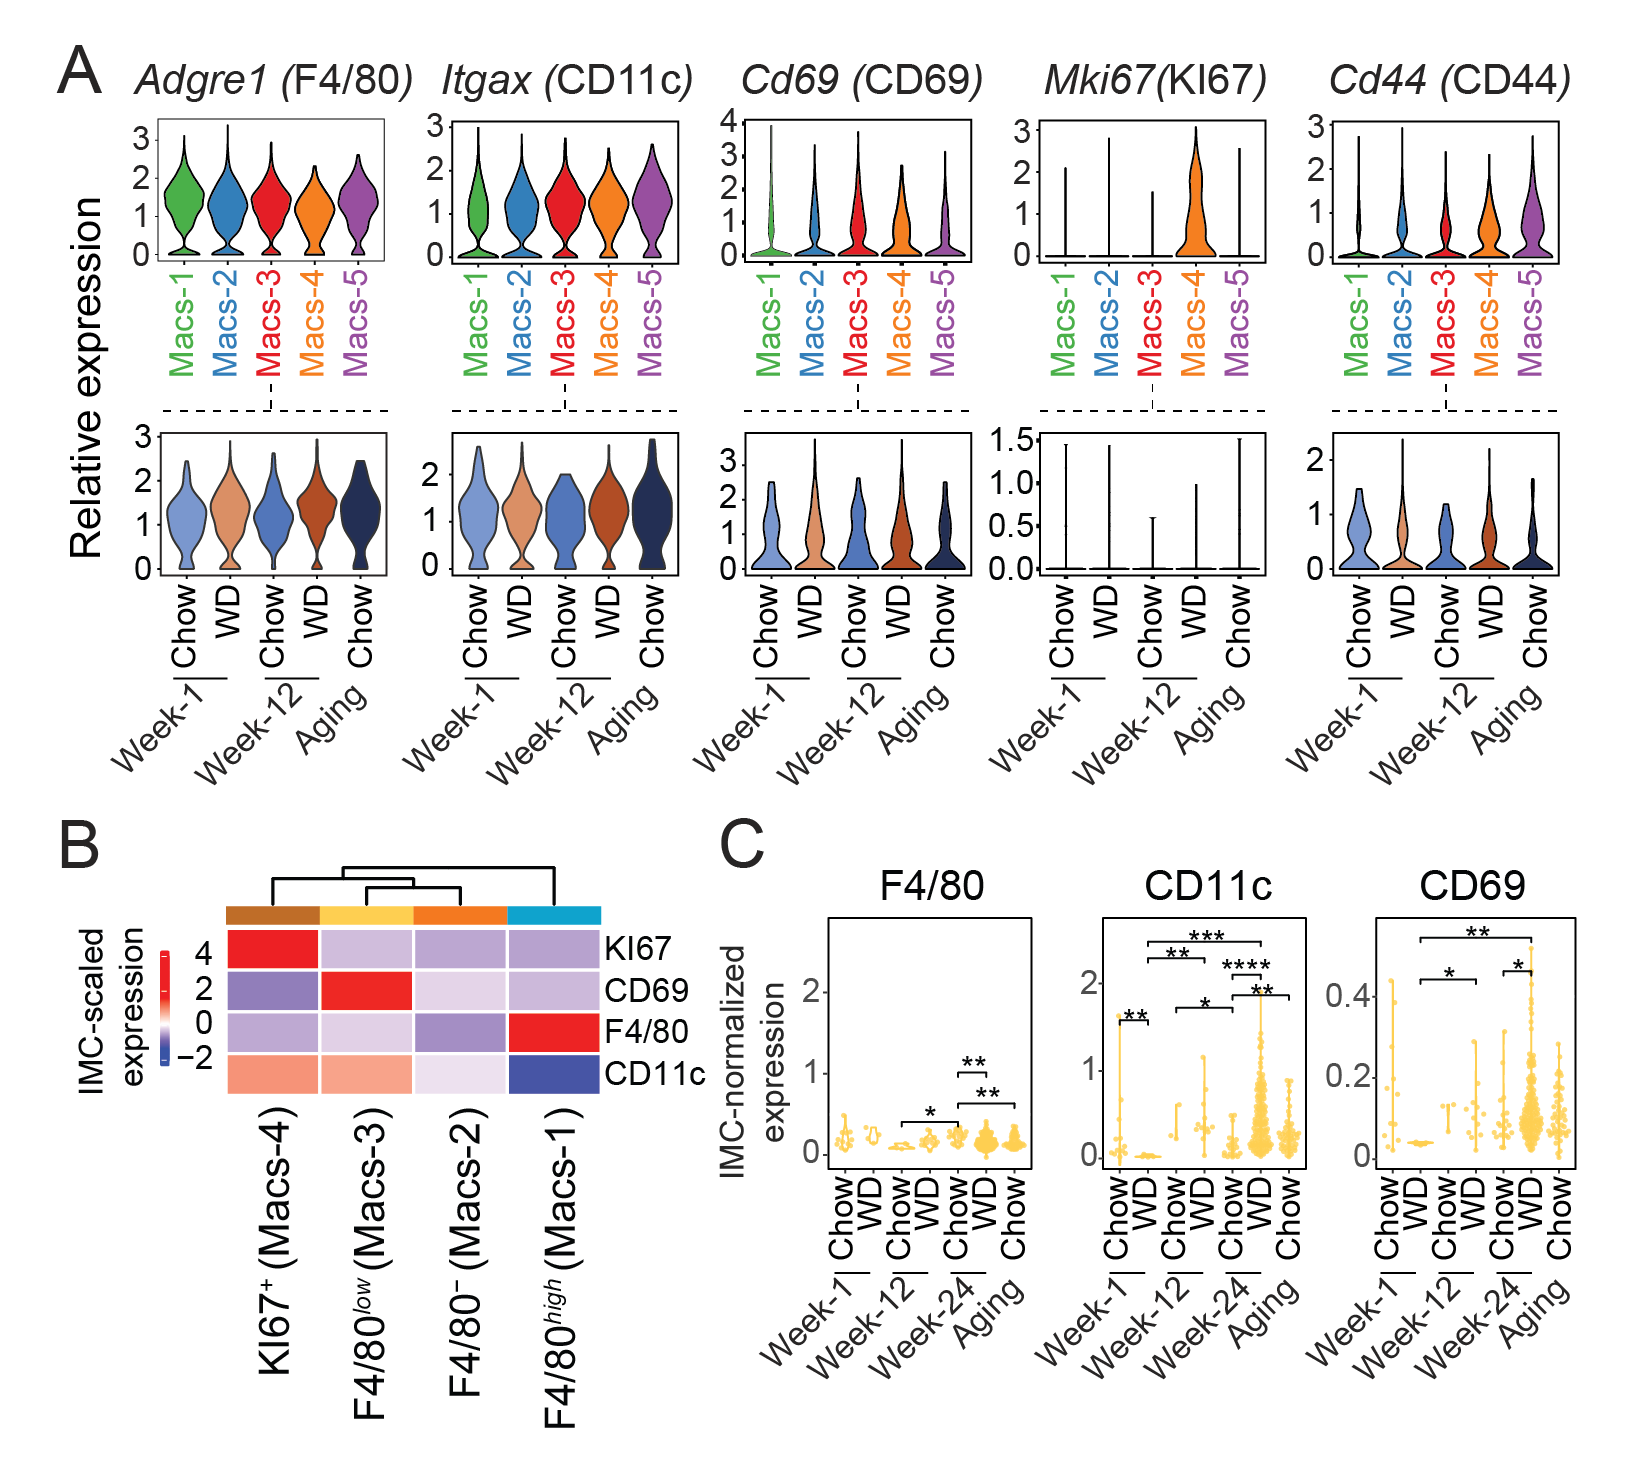
\includegraphics[width=9cm,height=11cm,keepaspectratio]{Chapter4/Fig/F2-4-01.png}%
% }[t]%

% \begin{wrapfigure}{r}{0.5\textwidth}
% 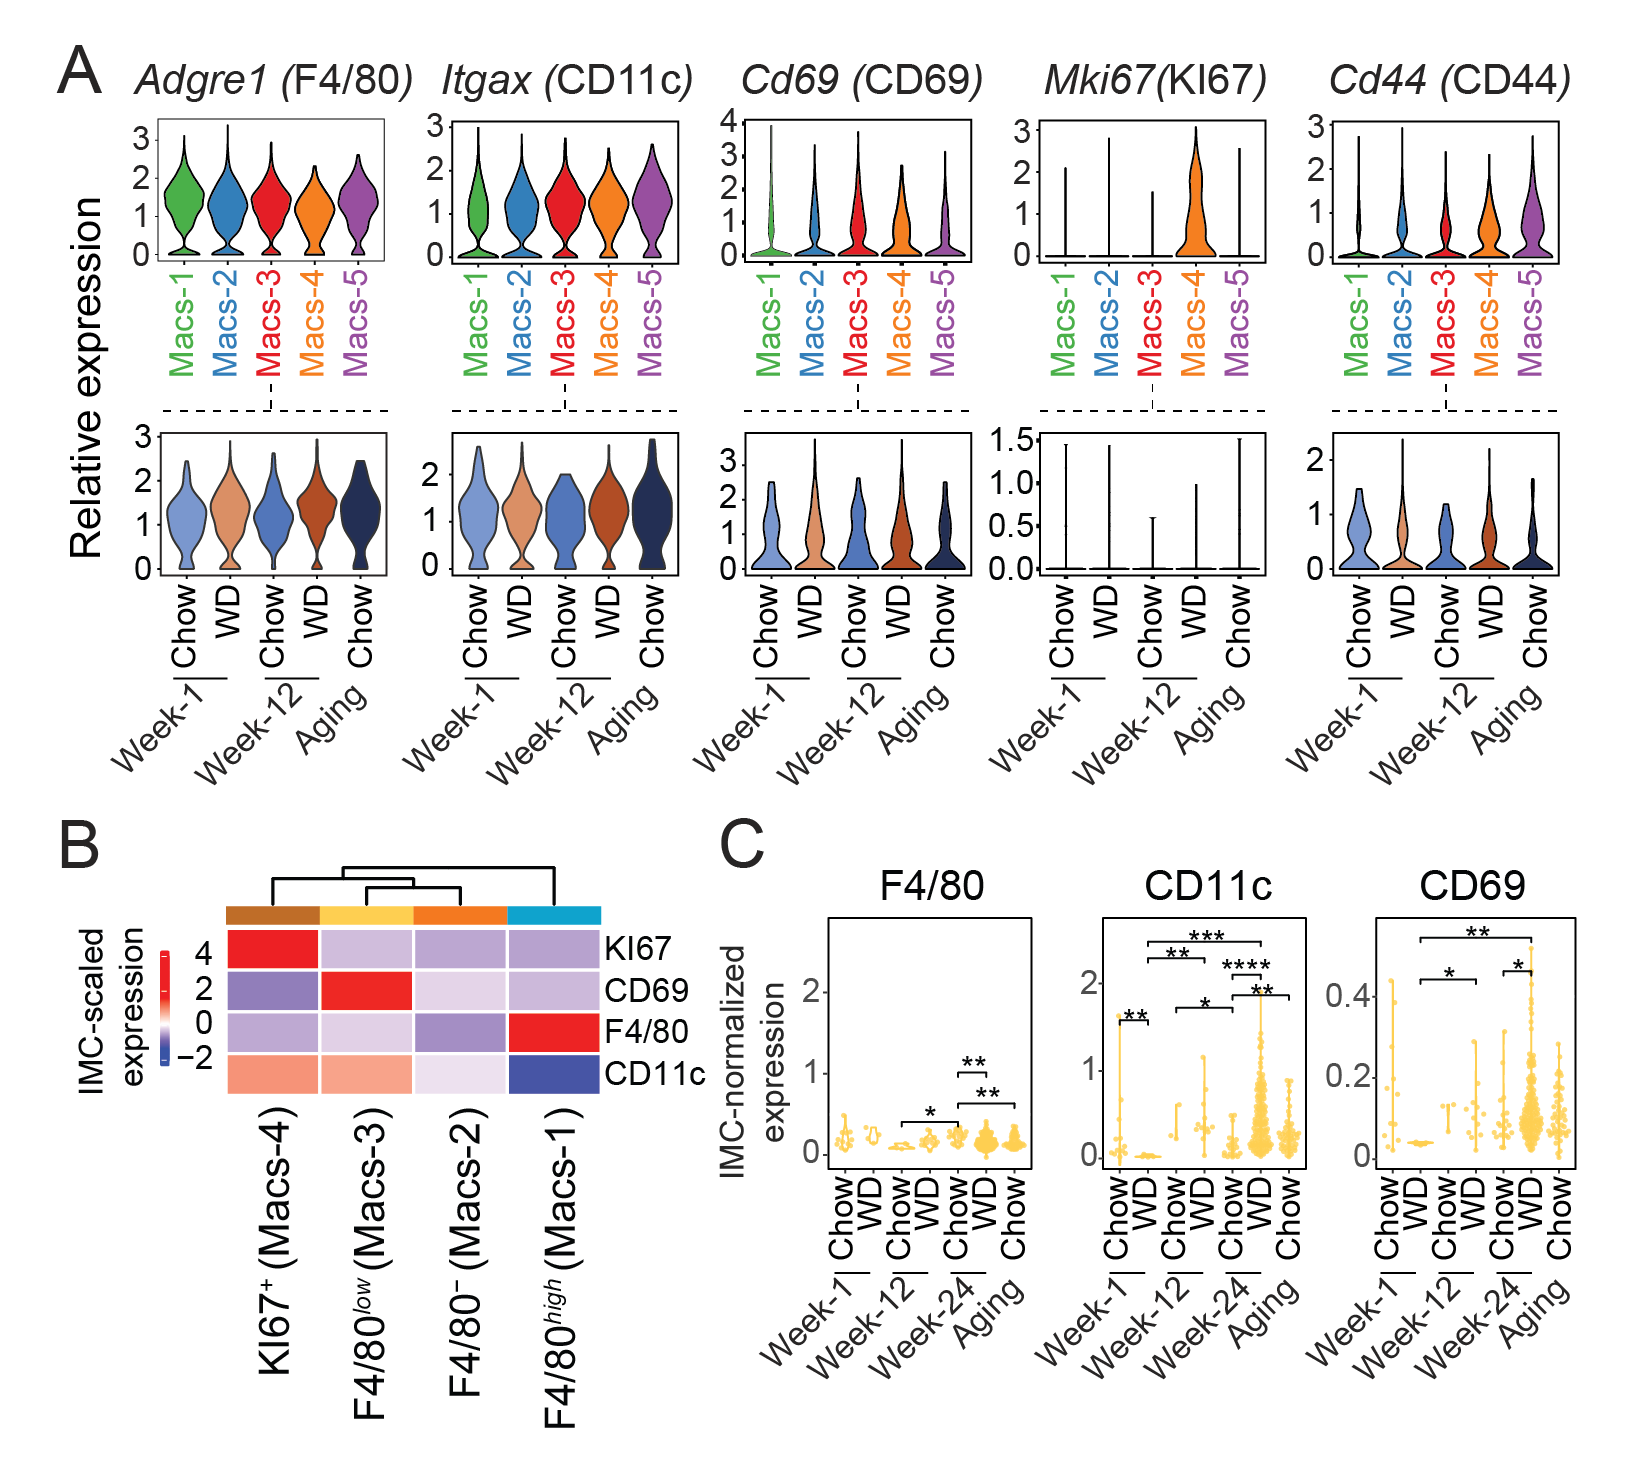
\includegraphics[width=9cm,height=11cm,keepaspectratio]{Chapter4/Fig/F2-4-01.png}
% \caption[]{\textbf{Linking macrophage sub-populations between scRNA-seq and IMC analyses.}}
% \label{fig2-4}
% \end{wrapfigure}




To further confirm the resemblance between the Macs-3 and F4/80\textsuperscript{\textit{low}} sub-populations, we undertook a comparative analysis of their inflammatory signatures in the context of WD feeding and aging conditions. The Macs-3 sub-population manifested an augmented inflammatory phenotype under both conditions, as evidenced by the up-regulated gene expression of CD11c (\textit{Itgax}) and CD69 (\textit{Cd69}) (\textbf{Fig. \ref{fig2-4} A, bottom}). This inflammatory modulation parallels observations in the F4/80\textsuperscript{\textit{low}} cells as elucidated from the IMC analysis (\textbf{Fig. \ref{fig2-4} C}).\\


% \begin{SCfigure}[][h]
% \centering
% 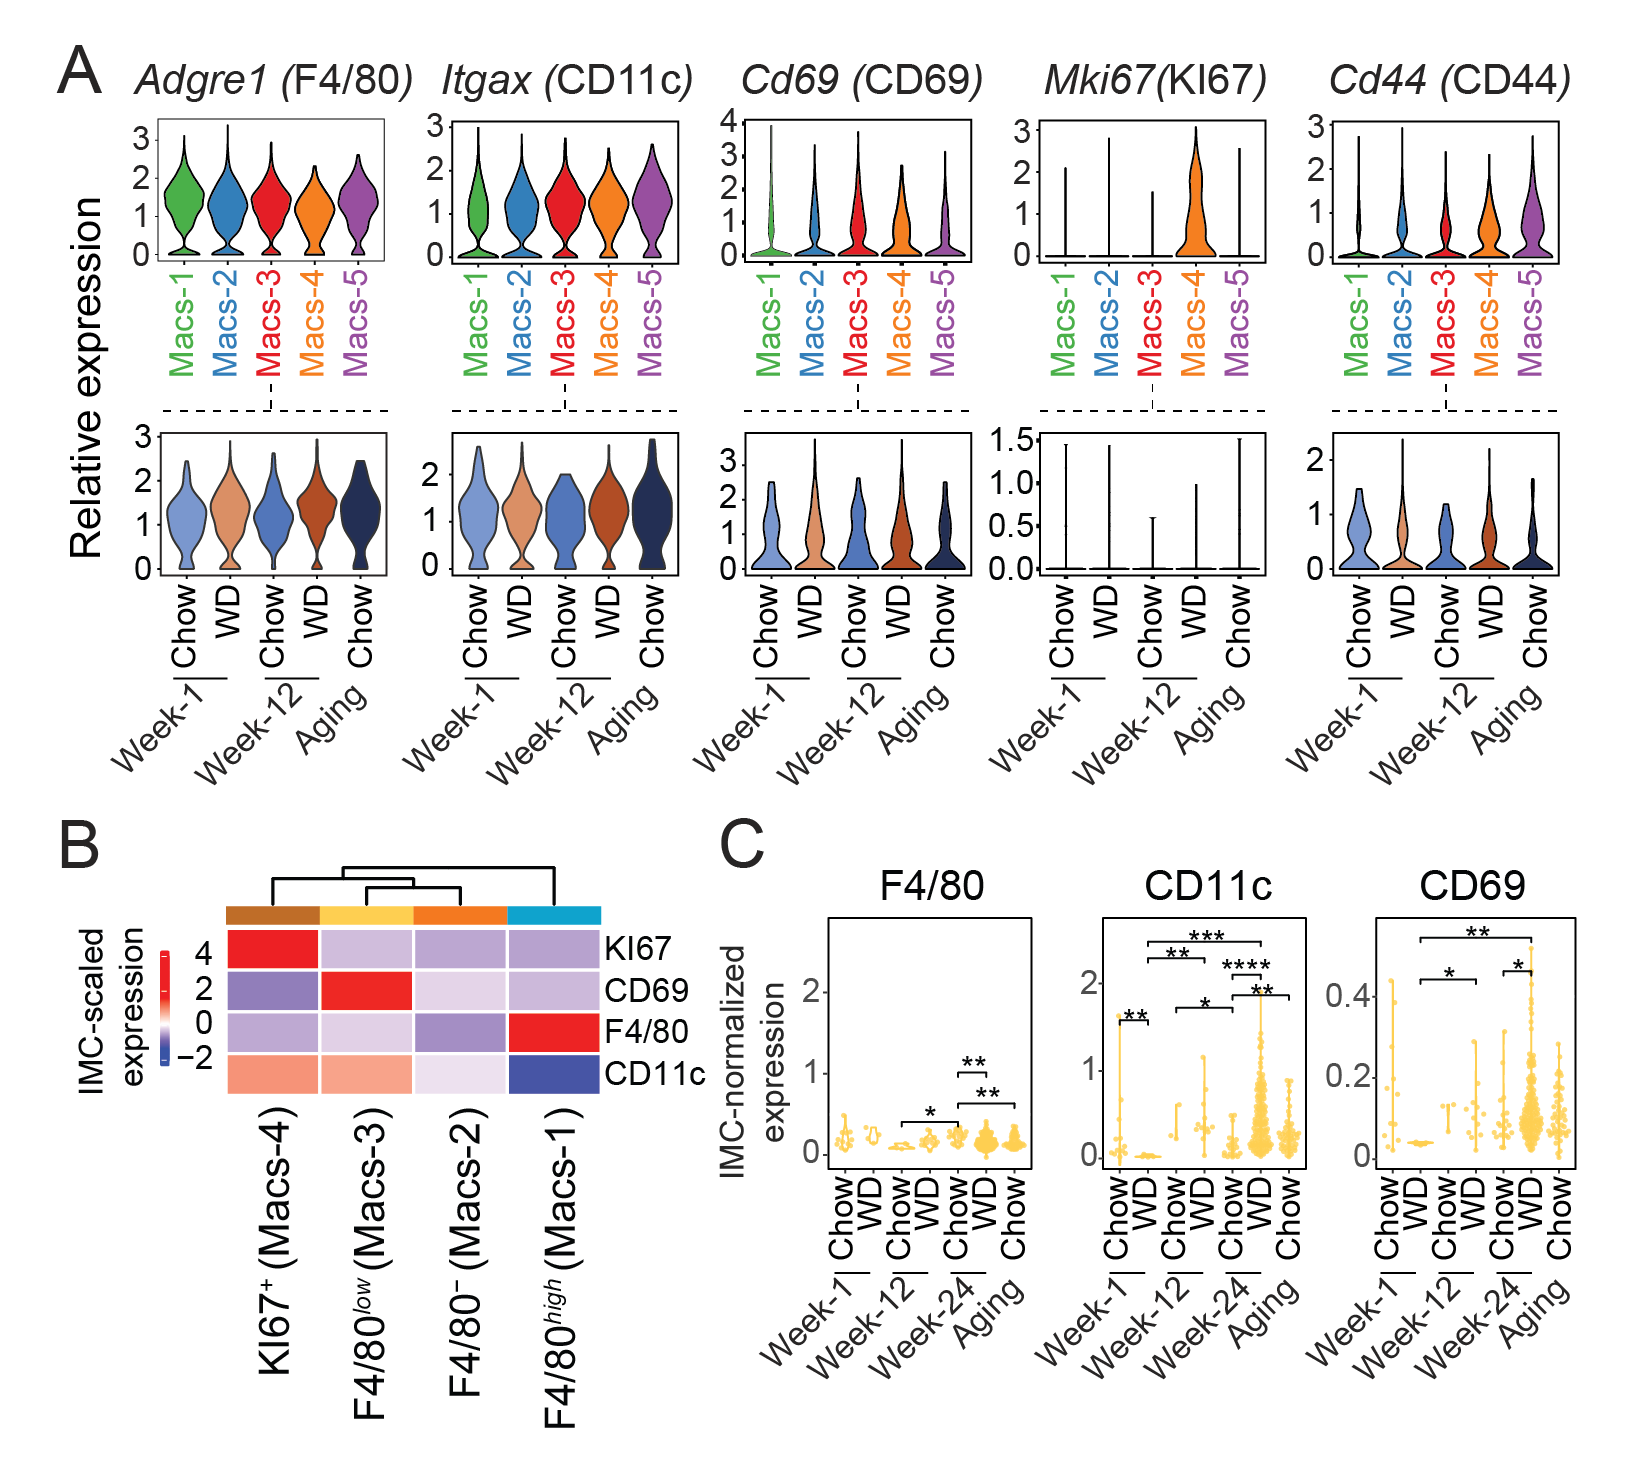
\includegraphics[width=8cm]{Chapter4/Fig/F2-4-01.png}
% \caption[res-macs2]{\textbf{Linking macrophage sub-populations from scRNA-seq to IMC}\\
% \textbf{(A)} Violin plots depicting the normalized expression levels of genes with corresponding channels in the IMC panel. The top plots compare these levels across various macrophage sub-populations, and the bottom plots display their expression in the Macs-3 population under different experimental conditions. \textbf{(B)}Heatmap showing z-scored expression of selected IMC channgels across the four macrophage sub-populations identified in the IMC analysis. Corresponding macrophage sub-populations from scRNA-seq analysis are indicated in parantheses. \textbf{(C)} Violin plots of \textit{arcsinh} transformed expression of selected IMC channels in the F4/80\textsuperscript{\textit{low}} macrophage sub-population from the IMC analysis across experimental conditions. *p<0.05, **p<0.01, ***p<0.001 and ****p<0.0001. p-values were calculated using the Wilcoxon rank-sum test with Bonferroni correction.} 
%  \label{fig2-4}
% \end{SCfigure}

% \begin{SCfigure}[1][h]
% \centering
% \caption[res-macs2]{\textbf{Linking macrophage sub-populations from scRNA-seq to IMC}. \textbf{(A)} Violin plots depicting the normalized expression levels of selected markers with corresponding channels in the IMC panel. The top plots compare these levels across various macrophage sub-populations, and the bottom plots display their expression in the Macs-3 population under different experimental conditions. \textbf{(B)}Heatmap showing z-scored expression of selected IMC channgels across the four macrophage sub-populations identified in the IMC analysis. Corresponding macrophage sub-populations from scRNA-seq analysis are indicated in parantheses. \textbf{(C)} Violin plots of \textit{arcsinh} transformed expression of selected IMC channels in the F4/80\textsuperscript{\textit{low}} macrophage sub-population from the IMC analysis across experimental conditions. * p<0.05, ** p<0.01, *** p<0.001 and **** p<0.0001. p-values were calculated using the Wilcoxon rank-sum test with Bonferroni correction.
% }
% 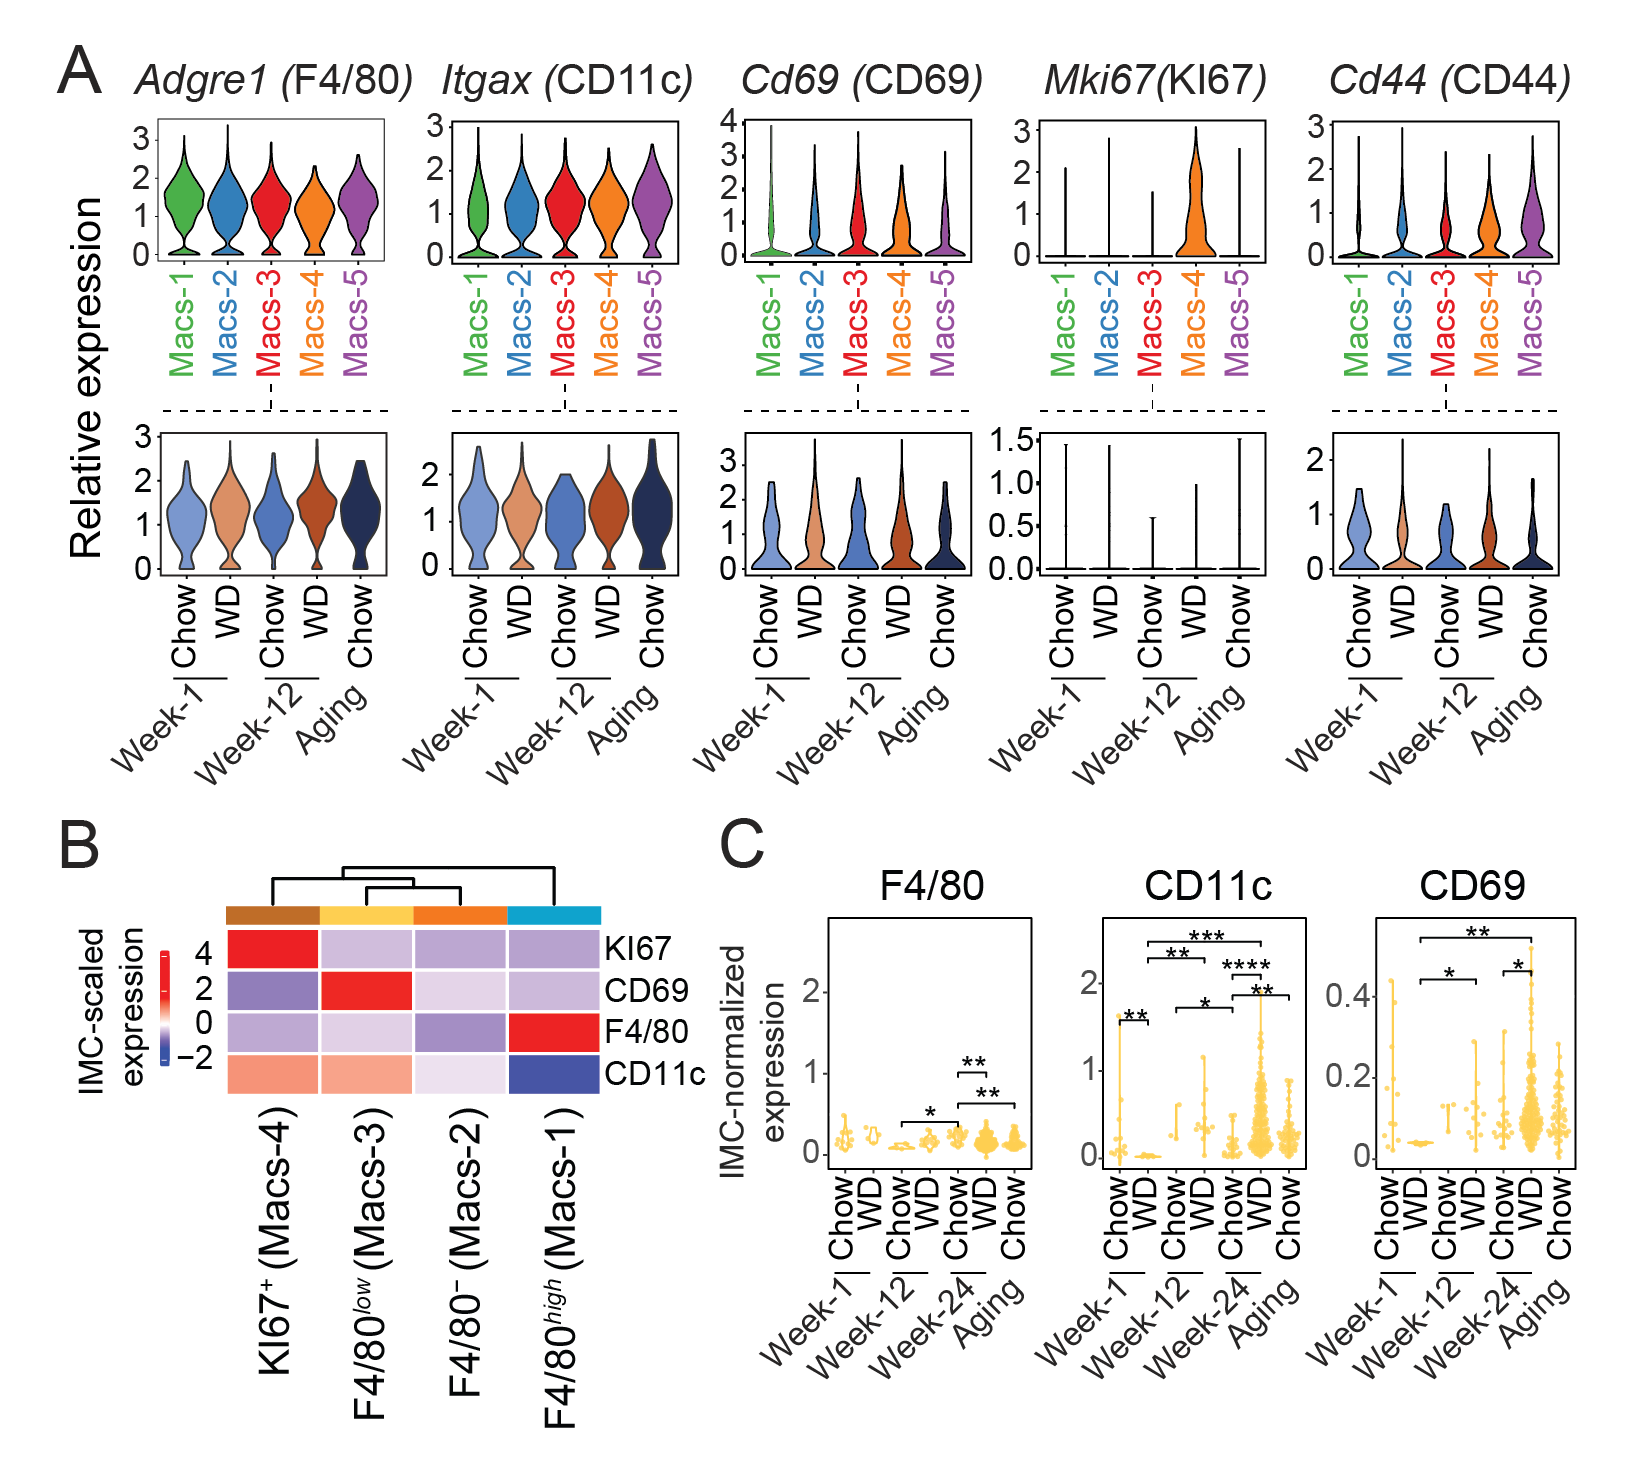
\includegraphics[width=0.6\textwidth]{Chapter4/Fig/F2-4-01.png}
% \label{fig2-4}
% \end{SCfigure}

Interestingly, despite Macs-2 exhibiting a lower activation profile compared to Macs-3, WD feeding resulted in a stronger expression of genes coding for inflammatory cytokines and chemokines in Macs-2 (Figure S4D,E). In contrast, this induced upregulation of cytokine genes observed in Macs-2 under WD feeding conditions is not evident in the aging condition (Figure S4F). The Macs-2 subtype also showed such non-canonical type 1 interferon responses, evident in the upregulated Socs3 expression one week after starting WD feeding (Figure S4D). Intriguingly, the WD triggered various inflammatory cytokine and chemokine gene expression, persisting twelve weeks into overnutrition (Figure S4E). In contrast, while Macs-2 in aging conditions exhibited signs of immune cell activation, it did not demonstrate cytokine expression (Figure S4F).\\

Collectively, our findings underscore age-related accumulation and activation of \textbf{inflammatory F4/80\textsuperscript{\textit{low}} macrophages} within pancreatic islets - a phenomenon that is markedly amplified under over-nutrition conditions.

% \subsubsection{Demultiplexing donors from pooled experiments} 
% \st{Interestingly, despite Macs-2 exhibiting a lower activation profile compared to Macs-3, WD feeding resulted in a stronger expression of genes coding for inflammatory cytokines and chemokines in Macs-2 (Figure S4D,E). In contrast, this induced upregulation of cytokine genes observed in Macs-2 under WD feeding conditions is not evident in the aging condition (Figure S4F)}


% In the considered pooled experimental design, cells from multiple donors are differentiated together in the same experiment. 
% To be able to link the genetic background of an individual with their transcriptional profile we need to map the cells back to their donor of origin, without the use of any barcode.
% Indeed, we find that for the large majority of cells the RNA-seq reads map to a sufficient number of common genetic variants for us to reliably assign each cell to its original donor.
% In particular, assignment of cells to donors was performed using Cardelino \cite{mccarthy2020cardelino}. 
% In short, Cardelino estimates the posterior probability of a cell originating from a specific donor using common genetic variants in \gls{scrnaseq} reads, while employing a Bayesian beta binomial-based approach to account for technical factors such as differences in read depth, allelic drop-out, and sequencing accuracy. 
% To perform donor assignment, we considered a larger set of \gls{hipsci} lines with genotype information (n=490), including the 126 lines used in this study. 
% A cell's assignment to a donor was considered successful if the model identified the match i) with posterior probability > 0.9, and ii) using a minimum of 10 informative variants. 
% Cells for which the donor identification was not successful were discarded and not considered for further analyses.
% Across the entire dataset, 99\% of cells that passed RNA QC steps (see below) were successfully assigned to a donor.
% In some cases, unexpected donor assignment (where several cells from one experiment were found to be assigned to none of the 4-6 donors used in that experiment) allowed me to identify (and correct) plate swaps that happened in the lab, without losing any data (\textbf{Fig. \ref{fig:plate_swap}}).

% \begin{figure}[h]
% \centering
% \includegraphics[width=14cm]{Chapter4/Fig/cardelino_example.png}
% \caption[Demultiplexing donors]{\textbf{Demultiplexing donors}.\\
% Example of how donor assignment of cells helped identifying a plate swap.
% To explore the results of the donor assignment algorithm \cite{mccarthy2020cardelino}, I plotted cells along two axes: on the x axis, the posterior probability of being assigned to a certain donor, on the y the number of common variants found on \gls{scrnaseq} reads used to perform the assignment.
% Because we know for each experiment which lines are supposed to have been differentiated, we can colour cells based on whether the donor they have been assigned to was used in the specific experiment or not.
% On the left, an example of a correct donor assignment: most cells are assigned to one of the correct donors\footnotemark and the few that are not had very few usable genetic variants.
% On the right, the donor assignment is apparently incorrect.
% Most cells were assigned to donors that were not differentiated in the experiment, in many cases with a high level of confidence and using many variants, which would generally indicate high quality cells.
% Indeed, investigating further we realised that all cells were assigned to donors that all belonged to the same experiment, but that it was a different experiment.
% The wrong label was assigned in the lab: run 225216 actually contained cells from experiment 43 and not 39.
% By resolving this computationally, we avoided mistakes and retained all of the cells from this sequencing run, which would have otherwise been discarded.}
% \label{fig:plate_swap}
% \end{figure}


%\subsubsection{Flow cytometry}

% The success of the differentiation protocol was validated using expression of two protein surface markers, a pluripotency marker, Tra-1-60, and a marker of definitive endoderm, CXCR4. 
% We note that while cells were gated using the two markers, we did not discard any cells based on their expression. 
% In contrast, the first cell QC step performed using \gls{facs} consisted in identifying dead cells based on 7AAD\footnote{Staining with 7AAD is used a cell viability assay.
% 7AAD cannot readily pass through intact cell membranes, thus only cells with compromised membranes will stain.} using \gls{facs} staining.
% These were discarded and were not plated. 
% \gls{facs} data were analysed using the openCyto package, implemented in R \cite{finak2014opencyto}.
% The \gls{facs} gating strategy we used is illustrated in \textbf{Fig. \ref{fig:endodiff_facs_strategy}}.

% \begin{figure}[h]
% \centering
% \includegraphics[width=14cm]{Chapter4/Fig/endodiff_facs_strategy.png}
% \caption[FACS gating strategy]{\textbf{FACS gating strategy}.\\
% Figure by Mariya Chhatriwala.
% \gls{facs} gating strategy: first, single cells were stained with 7AAD to exclude dead cells. 
% Unstained live cells were then used to gate for expression of Tra-1-60 and CXCR4.}
% \label{fig:endodiff_facs_strategy}
% \end{figure}


% \newpage

% % footnote from plate swap figure (to make it appear on right page)
% \footnotetext{A cell technically could still have been assigned to a wrong donor within the correct experiment, but given a threshold both on the variants used (> 10) and on the posterior probability (> 0.9) I deemed this unlikely.}

%\subsubsection{scRNA-seq feature quantification and quality control}

% Single cell profiles were obtained using the SmartSeq2 technology \cite{picelli2013smart}. 
% This is a plate-based technology that involves single cells being sorted into 384 independent wells on a plate. 
% Adaptors of raw \gls{scrnaseq} reads were trimmed using Trim Galore! \cite{galore2015wrapper, martin2011cutadapt, andrews2010fastqc}, using default settings. 
% Trimmed reads were mapped to the human genome (build 37) using STAR \cite{dobin2013star}. 
% Gene-level expression quantification was performed using Salmon \cite{patro2017salmon}. 
% Briefly, Salmon quantifies transcript- (rather than gene-) level expression levels, similar to Kallisto \cite{bray2016near}.
% Then, such values are summarised at a gene level (\gls{cpm}).\\

% We performed \gls{qc} of \gls{scrnaseq} profiles following a widely used pipeline (see \textbf{section \ref{sec:scrnaseq}}) using Bioconductor packages \textit{scater} and \textit{scran}, implemented in R \cite{lun2016step, mccarthy2017scater, lun2019singlecellexperiment}.  
% In particular, cells were retained for downstream analysis if they had at least 50,000 counts from endogenous genes, at least 5,000 genes with non-zero expression, if less than 90\% of counts came from the top 100 most highly-expressed genes, less than 15\% of reads mapped to mitochondrial (MT) genes, they had a Salmon mapping rate of at least 60\%, based on distribution observation and thresholding (\textbf{Fig. \ref{fig:endodiff_qc_distributions}}) \cite{luecken2019current}.
% Additionally, cells were only retained if they could be successfully assigned to a donor (QC1, \textbf{Fig. \ref{fig:endodiff_qc_workflow}}). \\ 

% I then performed an additional QC step, where I excluded all cells from plates and experiments that had overall low quality.
% In the case of plates sequenced twice, I retained the one with most cells.
% Finally, I retained plates that had enough cells for the majority of the donors considered (QC2, \textbf{Fig. \ref{fig:endodiff_qc_workflow}}). 

% \begin{figure}[h]
% \centering
% \includegraphics[width=16cm]{Chapter4/Fig/endodiff_qc_examples.png}
% \caption[Distributions of QC metrics]{\textbf{Distributions of QC metrics}.\\
% Distributions of three exemplar QC metrics for six differentiation experiments (40-45).
% Shown are the cell distributions along the metrics (number of genes detected, percentage of counts from mitochondrial genes, Salmon \cite{patro2017salmon} mapping rate), as well as the thresholds we used as dotted lines, stratified by day and experiment.
% One can immediately spot how poor quality plates\footnotemark  perform similarly badly across all metrics (i.e. < 5,000 genes detected, <60\% reads mapped by Salmon).}
% \label{fig:endodiff_qc_distributions}
% \end{figure}

% \begin{figure}[h]
% \centering
% \includegraphics[width=16cm]{Chapter4/Fig/endodiff_qc_workflow.png}
% \caption[QC workflow]{\textbf{QC workflow}.\\
% Two stages of cell QC.
% First, at the level of single cells, all QC metrics and thresholds are indicated.
% 61\% of cells passed QC1.
% Second, at the experiment/plate level.
% If plates had many cells not passing QC1 they were considered poor quality batches and removed altogether.
% This stage removed far fewer cells, with 96\% of cells considered passing QC2.}
% \label{fig:endodiff_qc_workflow}
% \end{figure}


%\subsubsection{scRNA-seq processing}

% SmartSeq2 data do not include \glspl{umi}, which can be used to accurately detect PCR duplicates and quantify transcript abundance \cite{smith2017umi, islam2014quantitative, kivioja2012counting}. 
% In the absence of \glspl{umi}, we can borrow information from cells with similar total number of reads and correct for overall library size. 
% Such size factor normalisation of counts was performed using \textit{scater} \cite{mccarthy2017scater}. 
% %  \\
%  % footnote from qc examples figure (to make it appear on right page)
% \footnotetext{e.g. cells from day0, experiment 42.}
% Expressed genes with an HGNC symbol were retained for analysis, where expressed genes in each batch of samples were defined based on (i) raw count >100 in at least one cell prior to cell QC (i.e. \textbf{Fig. \ref{fig:endodiff_qc_workflow}}) and (ii) average log2(CPM+1) >1 after cell QC. 
% Normalised CPM data were log transformed (log2(CPM+1)) for all downstream analyses. 
% As a last QC step, we considered possible differences between cell lines derived from healthy and diseased donors. 
% Specifically, a subset of 11 cell lines in our dataset were derived from monogenic neonatal diabetes patients, and differentiated together with cell lines from healthy donors across 7 differentiation experiments (out of 28). 
% There was no significant difference in differentiation efficiency (see \textbf{section \ref{sec:endodiff_differentiation_efficiency}}) between healthy and neonatal diabetes lines in these experiments (p value > 0.05), and cells from both sets of donors overlapped in principal component space (\textbf{Fig. \ref{suppl_fig:pca_diabetes_lines}}). 
% Thus, we included cells from all donors in our analyses, irrespective of disease state.


%\newpage

\section{Aging and metabolic stress activate distinct Type-1\\IFN responses in accumulating inflammatory macrophages.}
\label{sec:endodiff_overview}
The observed enrichment of the Type-1 IFN-responsive macrophage sub-population (Macs-3) during both WD feeding and aging suggests active IFN signaling in the pancreatic islets. To delve deeper into how Macs-3 responds to these pro-inflammatory conditions, we performed \gls{dge} analysis between WD and chow fed cohorts after 1 and 12 weeks of feeding, and between the chow fed aged cohort and the non-aging controls, which include the chow fed groups at 1 and 12 weeks. We observed that both overnutrition and aging amplified the Type-1 IFN response in Macs-3 (Figure 4A-C). Importantly, while aging elicited a canonical response, evidenced by the upregulation of the \textit{Stat1} and \textit{Cxcl9} gene expression (Figure 4C), WD feeding initiated a different Type-1 IFN response, involving the up-regulation of the negative feedback regulator, \textit{Socs3} and other \textit{Stat3} target genes such as \textit{Cxcl10} and \textit{Il1b} (Figure 4A,B) (references).

\begin{figure}[H]
\centering
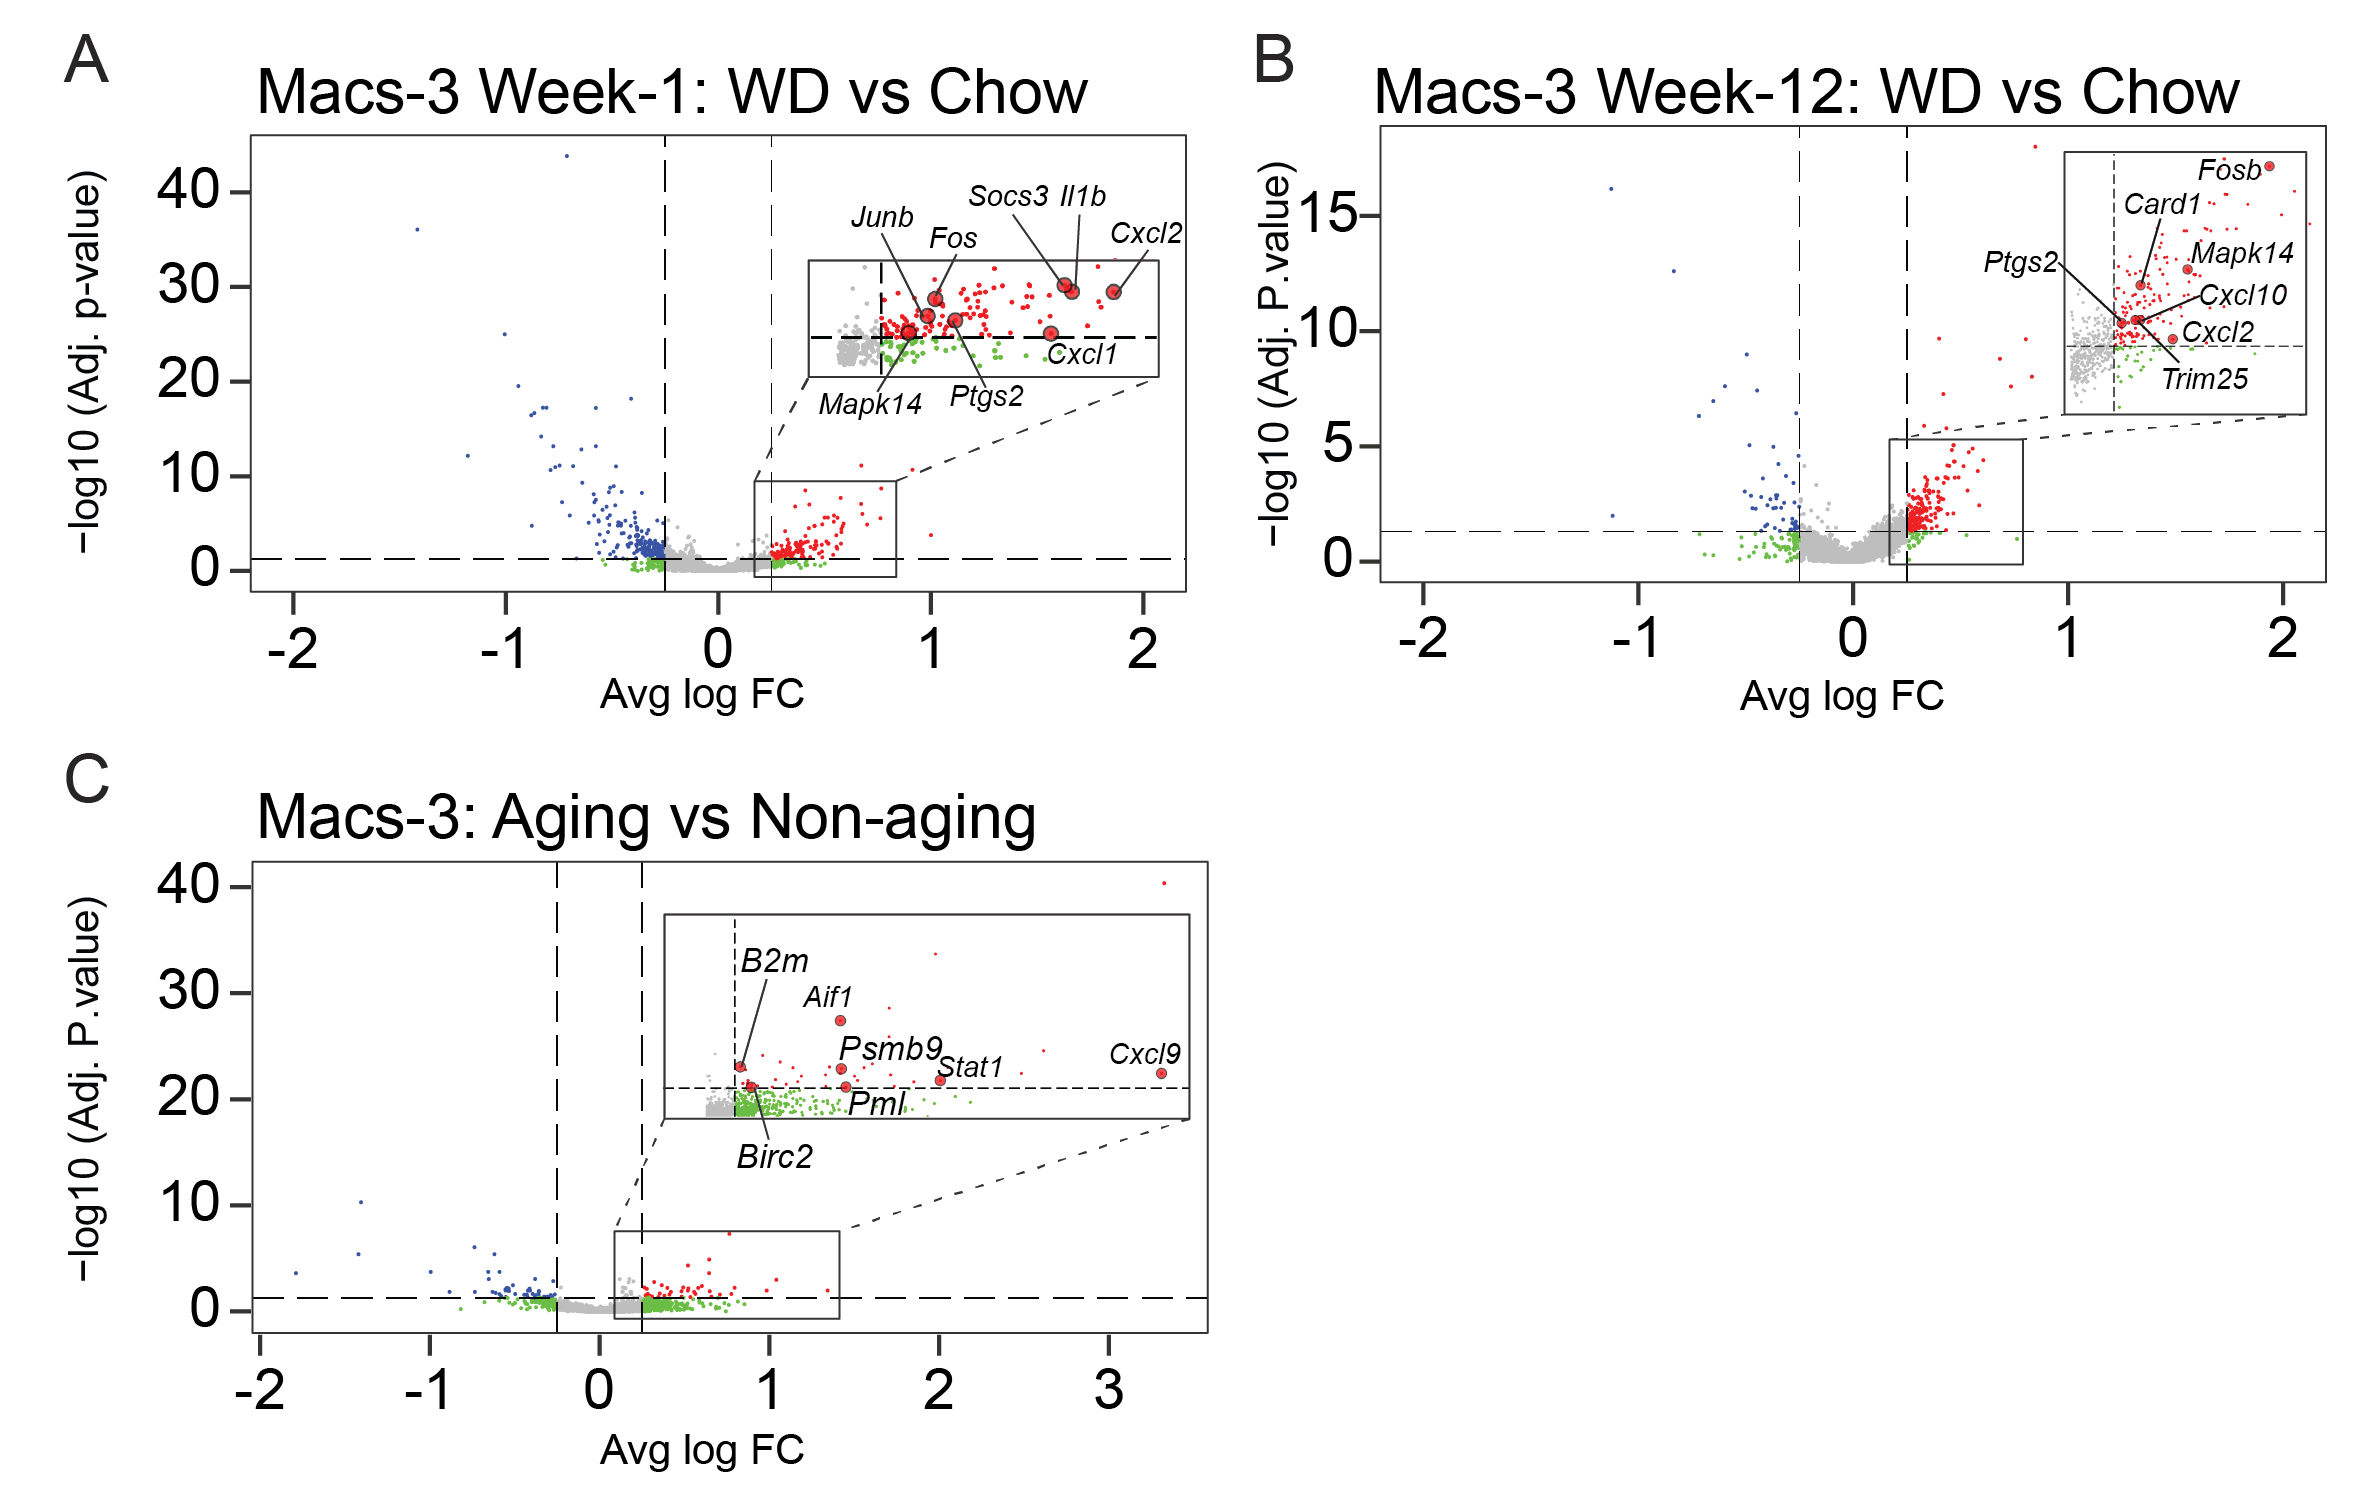
\includegraphics[width=\linewidth]{Chapter4/Fig/F2-11-01.png}
\caption[res-macs3-1]{\textbf{Differential Gene Expresssion (DGE) analysis of Macs-3}
}
\label{fig2-11}
\end{figure}


We further explored the similarities and differences between the inflammatory responses during overnutrition and aging. In that regard, we clustered all the differentially expressed genes in Macs-3 cells according to their expression patterns across all tested conditions and time-points, and identified gene modules comprising of analogous expression dynamics (\textbf{Fig.\ref{fig2-12} A}). Intriguingly, we were able to differentiate between transcriptomic alterations orchestrated specifically by aging (\textbf{km-3}, \textbf{km-5}, and \textbf{km-9}) and those induced by WD feeding (\textbf{km-4}, \textbf{km-6}, and \textbf{km-10}). Furthermore, we also identified gene modules with similar functions under both these conditions (\textbf{km-1}, \textbf{km-7}, and \textbf{km-8}). We functionally annotated both the condition-specific and common gene modules using GO and pathway enrichment analysis (\textbf{Fig.\ref{fig2-12} B}). Our analysis revealed that under both WD feeding and aging conditions, Macs-3 exhibited a reduction in the expression of genes involved in canonical glycolysis (\textbf{km-1}), suggesting a consistent metabolic reprogramming across these conditions. Additionally, both stressors led to decreased expression of genes involved in cytoskeletal organization and those related to RNA splicing. Furthermore, both conditions induced an increase in the expression of genes promoting cell proliferation, thereby likely explaining the observed expansion of Macs-3 within the islets (\textbf{Fig.\ref{fig2-12} B}).

\begin{figure}[H]
\centering
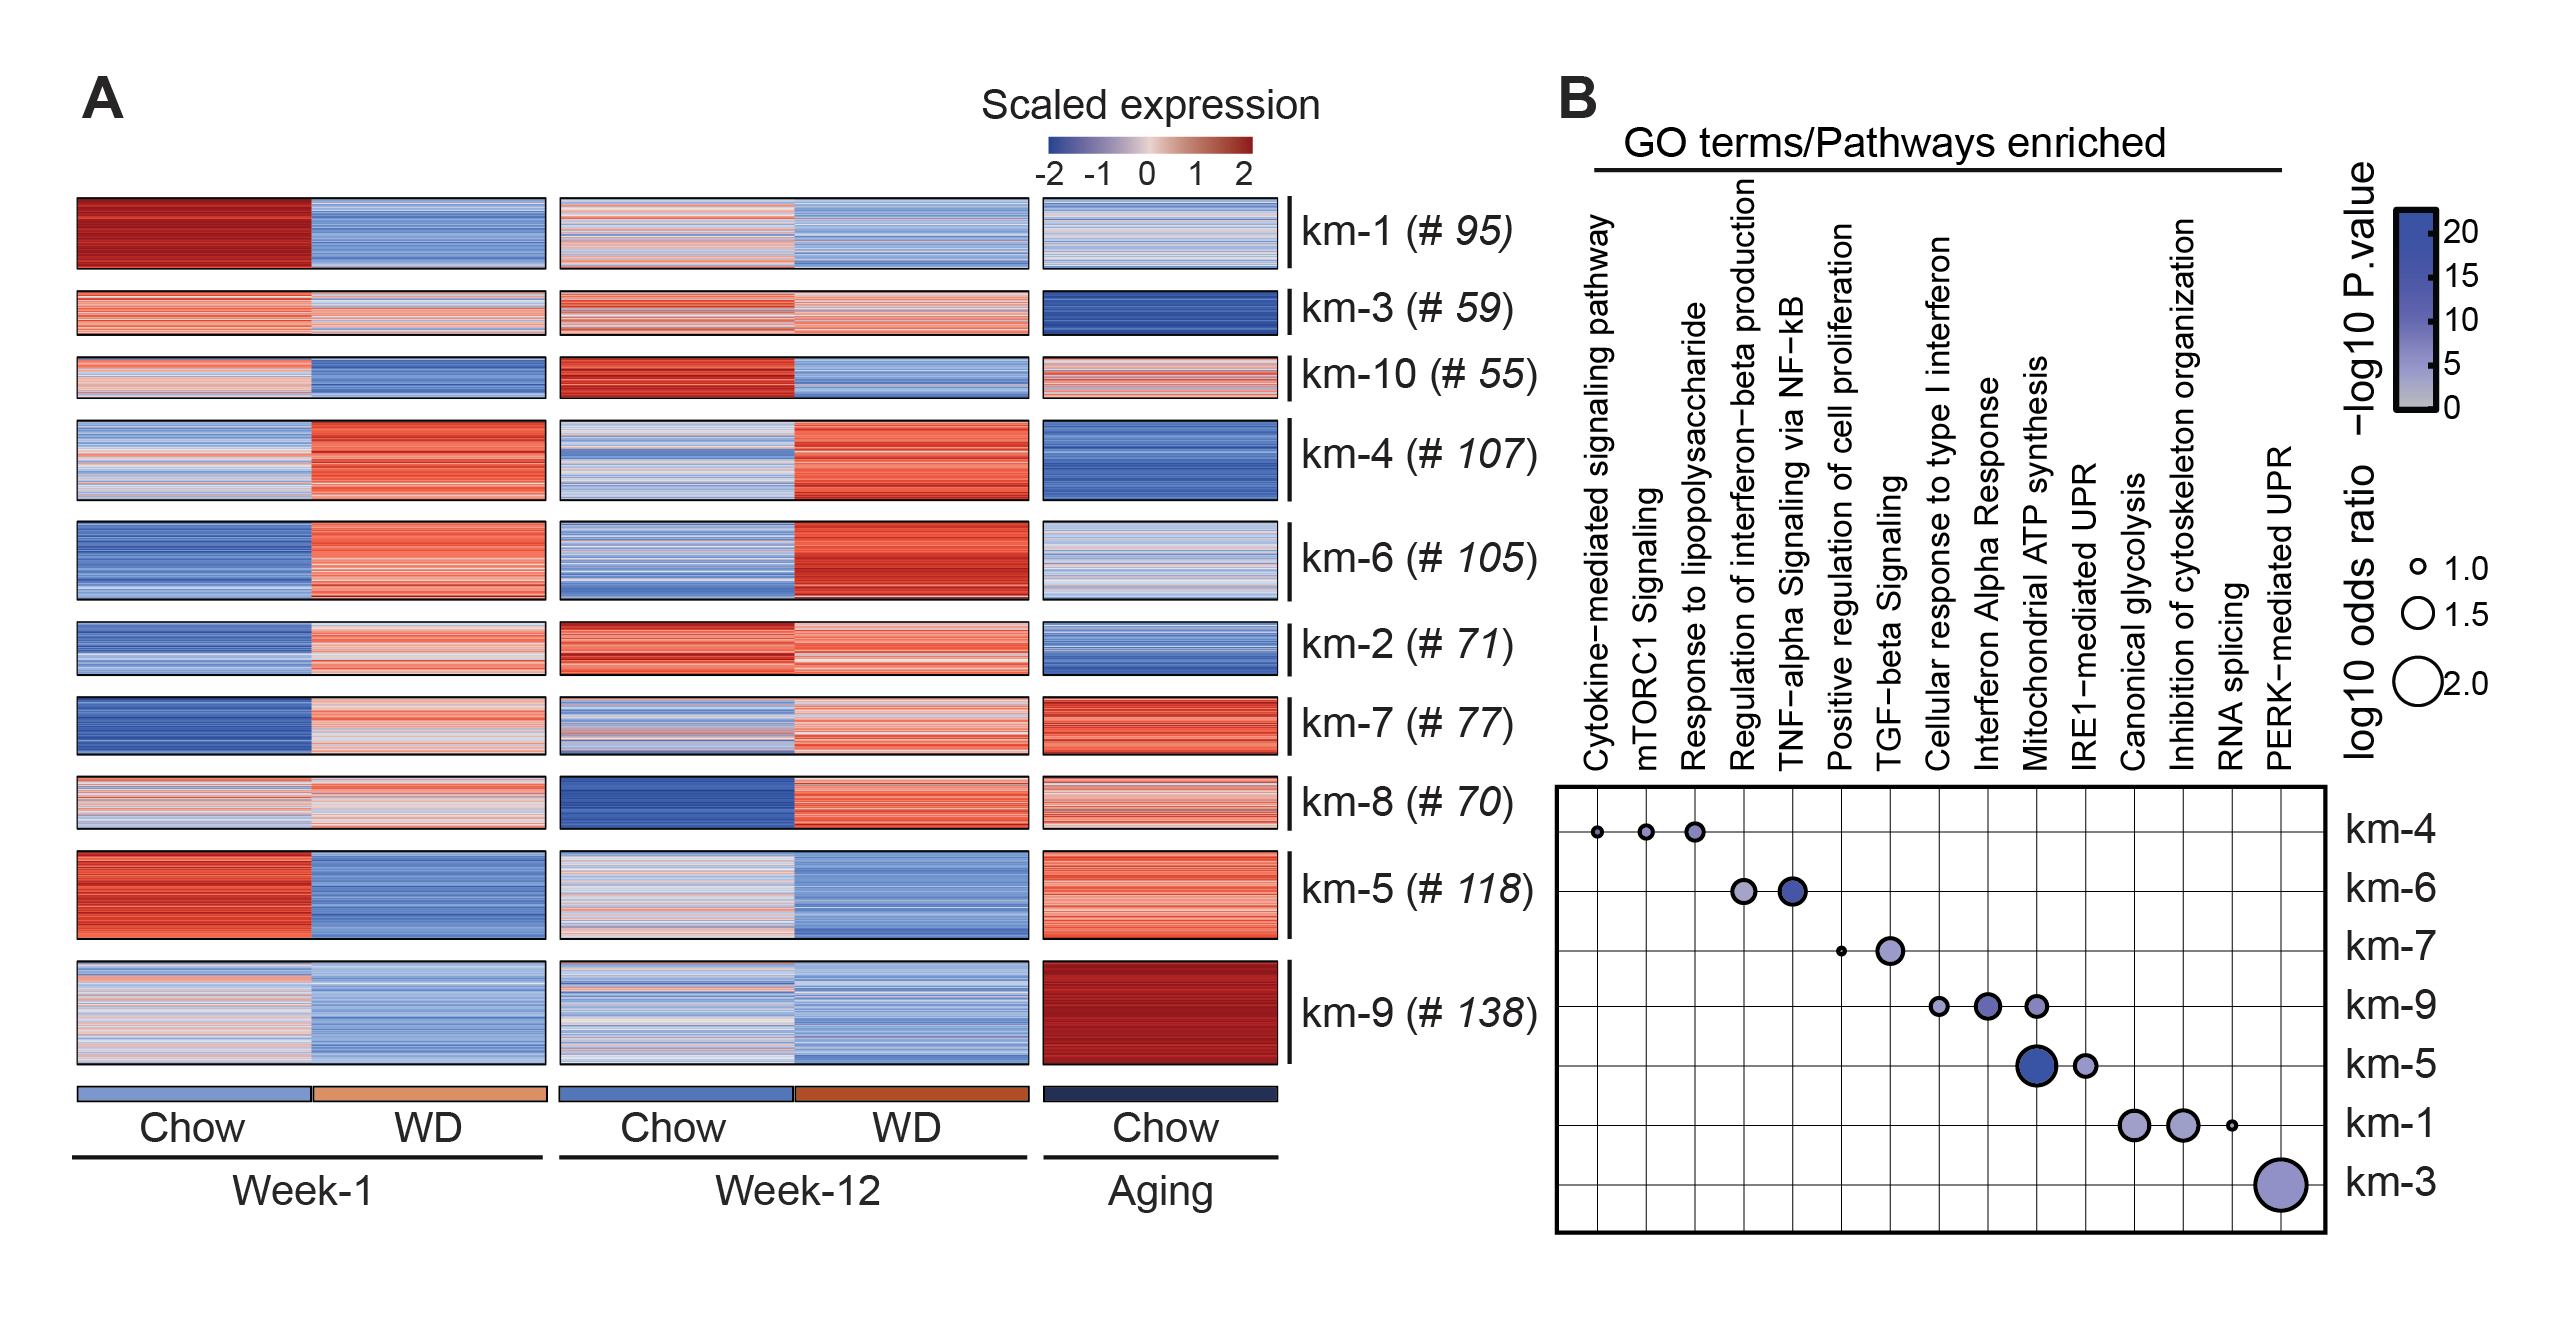
\includegraphics[width=\linewidth]{Chapter4/Fig/F2-11-02.png}
\caption[res-macs3-2]{\textbf{Dsimilarities and differences between the inflammatory responses during overnutrition and aging}
}
\label{fig2-12}
\end{figure}


Consistent with the results from our pair-wise \gls{dge} analysis (Figure 4A-C), Macs-3 did activate the Type-1 IFN response under both WD and aging conditions. However, this response was notably intensified during aging (\textbf{km-9}). This heightened response is likely attributed to the enhanced canonical response and the absence of feedback inhibition by \textit{Stat3/Socs3} (Figure 4A), which was observed in WD. It might also be explained by the aging-specific attenuation of the PERK pathway (\textbf{km-3}), which has been proposed to maintain an immunosuppressive phenotype in macrophages (PMID: 35228694). Conversely, the overnutrition condition uniquely triggered the \textit{mTORC1} pathway (\textbf{km-4}) in Macs-3, further suggesting that it represents a non-canonical Type-1 IFN response (PMID: 33329603). Furthermore, WD feeding specifically triggered the activation of genes in the \textit{TNFα/NFkB} signaling pathway (\textbf{km-6}) in Macs-3, a change that was not evident during aging. This highlights the potential involvement of additional pro-inflammatory cytokines during metabolic stress as opposed to inflammaging.\\\\
In summary, our analysis revealed an activation of the canonical Type-1 IFN response during inflammaging. While overnutrition can accelerate a similar process, it likely triggers a non-canonical signaling cascade, as indicated by the activation of the \textit{Stat3} and \textit{mTOR} pathways, thereby leading to a more pronounced inflammatory state.
\clearpage

% Following quality control (QC), 36,044 cells were retained for downstream analysis, across which 11,231 genes were expressed.
% At each time point, cells from between 104 and 112 donors were captured, with each donor being represented by an average of 286 cells (after QC, \textbf{Fig. \ref{fig:endodiff_stats}}). 
% The success of the differentiation protocol was validated using canonical cell-surface marker expression: consistent with previous studies \cite{chu2016single}, an average of 72\% of cells were TRA-1-60(+) in the undifferentiated state (day0) and an average of 49\% of cells were CXCR4(+) three days post differentiation (day3, \textbf{Fig. \ref{fig:endodiff_stats}}).
 
% \begin{figure}[htbp]
% \centering
% \includegraphics[width=14cm]{Chapter4/Fig/endodiff_stats.png}
% \caption[Overview of experimental metrics]{\textbf{Overview of experimental metrics.}\\
% Statistics for number of cells, donors, experiments, days, and combinations. 
% Cell counts are shown after quality control.
% Additionally, shown are the percentages of cells that are positive for TRA-1-60, a pluripotency marker, positive for CXCR4, a definitive endoderm marker, and  positive for CXCR4 and negative for TRA-1-60, across all cell lines and all experiments.}
% \label{fig:endodiff_stats}
% \end{figure}



% \newpage

% \subsection{Sources of variation} 
% \label{sec:endodiff_sources_of_variation}


% To identify the main sources of variation in our dataset we performed variance component analysis for each of the genes, using a linear mixed model.
% Variance component analysis revealed the time point of collection as the main source of variation, followed by the cell line of origin and the experimental batch (\textbf{Fig. \ref{fig:endodiff_vca}}).\\

% \begin{figure}[h]
% \includegraphics[width=10cm]{Chapter4/Fig/endodiff_variance_component.png}
% \caption[Variance Component Analysis]{\textbf{Variance Component Analysis}.\\
% Summary of variance component analysis results for each of 4,546 highly variable genes, using a linear mixed model fit to individual genes to decompose expression variation into
% time point of collection, cell line and experimental batch.
% The number of genes for which each factor explains 10\%, 20\%, 30\% and 40\% of the variance respectively is indicated.}
% \label{fig:endodiff_vca}
% \end{figure}

% Next, we performed \gls{pca} on our dataset.
% To do so, we first identified the top 500 \gls{hvgs} defined as the most variable genes given a mean-variance trend calculated across all genes, using the function \textit{trendVar} as implemented in the R package scran.
% Consistent with the results from the variance component analysis (\textbf{Fig. \ref{fig:endodiff_vca}}), the first principal component (PC1) was aligned with differentiation time, motivating its use to order cells by their differentiation status (hereafter `pseudotime', \textbf{Fig. \ref{fig:endodiff_pca}}).\\

% \begin{figure}[h]
% \centering
% \includegraphics[width=14cm]{Chapter4/Fig/endodiff_pca_overview.png}
% \caption[Overview of dataset.]{\textbf{Overview of dataset.}\\
% Principal component analysis of gene expression profiles for 36,044 QC-passing
% cells, coloured by the time point of collection.
% PC1 effectively captures differentiation time and is defined as pseudotime.}
% \label{fig:endodiff_pca}
% \end{figure}

% Pseudotime inference is a common step in the analysis of \gls{scrnaseq} data along differentiation and development: while single cells are single snapshots along time, with enough points and considering that cells differentiate at different rates, they can be used to reconstruct a trajectory.
% In this case, the nature of the short and linear differentiation process of our data (i.e. iPSC $\rightarrow$ mesendoderm $\rightarrow$ definitive endoderm) meant that PC1 captured the differentiation trajectory.
% For comparison, we did apply alternative pseudotime inference methods, which yielded similar orderings (\textbf{Fig. \ref{fig:endodiff_pseudotimes}}).
% Further validation of our inferred pseudotime was provided by the temporal expression dynamics of known marker genes that characterise endoderm differentiation, which was captured by our ordering of cells as expected (\textbf{Fig. \ref{fig:endodiff_stages}}).

% \begin{figure}[htbp]
% \centering
% \includegraphics[width=14cm]{Chapter4/Fig/endodiff_pseudotimes.png}
% \caption[Evaluation of pseudotime definition]{\textbf{Evaluation of pseudotime definition by comparison with alternative approaches.}\\
% (a) Comparison of the pseudotime defined based on principal component analysis with diffusion pseudotime (DPT) \cite{haghverdi2016diffusion}. 
% The diffusion map was generated using 15 nearest neighbours and the first 20 PCs across the top 500 most highly variable genes.  
% (b) Comparison of our defined pseudotime with an alternative measure of pseudotime based on projection of each cell on to a principal curve (using princurve as implemented in R \cite{hastie1989principal}) calculated using the first two principal components from the top 500 most highly variable genes. 
% (c) Comparison of our pseudotime to the average expression of 124 co-expressed genes associated with cell differentiation. 
% (d) Scatter plot-derived loess curves of \gls{facs} markers as a function of the our PCA-based pseudotime, showing expected trends.}
% \label{fig:endodiff_pseudotimes}
% \end{figure}

% \subsection{Defining discrete developmental stages}

% While the continuous measure of pseudotime nicely highlights the dynamics of gene expression over time, in order to map eQTL, and to be able to exploit methods similar to those described in the previous chapter (\textbf{Chapter  \ref{chapter3}}), it was also important to define homogeneous populations of cells that represent specific developmental stages.
% To do so, we assign our cells to one of three non-overlapping stages, corresponding to the three canonical stages of endoderm differentiation: \gls{ipsc}, mesendoderm (mesendo) and definitive endoderm (defendo).
% In particular, we utilise i) the ordering of cells along our inferred pseudotime ii) the expression of the previously described markers of differentiation progress and iii) the cell's day of collection to determine the cell assignment to each stage (\textbf{Fig. \ref{fig:endodiff_stages}}).
% Specifically, we assign all day0 cells to the iPSC cluster given their very high homogeneity.
% Next, cells were assigned to the mesendoderm stage if they were collected at either day1 or day2, and had pseudotime values corresponding to the peak expression of \textit{Brachyury} (\textit{T}) along pseudotime (pseudotime between 0.15 and 0.5, \textbf{Fig. \ref{fig:endodiff_stages}}).  
% Similarly, cells were assigned to definitive endoderm if they were collected at day2 or day3 and had pseudotime values higher than 0.7, corresponding to a pseudotime window with maximal expression of \textit{GATA6} (\textbf{Fig. \ref{fig:endodiff_stages}}).
% In total, we assigned 28,971 cells (about $\sim$80\% of all cells) to one of the three stages. 
% A smaller fraction of cells with intermediate pseudotime (between 0.5 and 0.7, n=7,073) could not be confidently assigned to a canonical stage of differentiation; these cells were largely collected at day2, at which stage rapid changes in expression profiles are expected, reflecting a transitional population of cells.
% I note that these cells were excluded for the purposes of the initial stage eQTL mapping (results in \textbf{section \ref{sec:endodiff_eqtl}}), but are included in all other analyses. 

% \vspace{2mm}

% \begin{figure}[h]
% \centering
% \includegraphics[width=14cm]{Chapter4/Fig/endodiff_stages.png}
% \caption[Developmental stages]{\textbf{Marker gene expression in pseudotime-based developmental states.}\\
% Expression of exemplar canonical markers for iPSC (\textit{NANOG}), mesendoderm (\textit{T}) and definitive endoderm (\textit{GATA6}) along pseudotime.
% Developmental stages were defined taking into consideration i) the day of collection, ii) the expression of canonical markers, and iii) the position along pseudotime.}
% \label{fig:endodiff_stages}
% \end{figure}

\section{β-cells display distinct inflammatory profiles in response to\\obesity and aging}
\label{sec:chp2_betacells}

To elucidate the similarities and differences in islet function at the transcriptomic level, we conducted an analysis on the β-cells derived from our scRNA-seq data. Following a sub-clustering analysis, we identified three β-cell sub-populations \textbf{(Fig. )}. Compared to previous single-cell analysis of murine islets [PMID: 32694693], we observed that our Beta-3 cells corresponded to a \textit{Cd81}\textsuperscript{+} immature beta cell population \textbf{(Fig. )}. Whereas both Beta-1 and Beta-2 represented mature beta cells, Beta-1 exhibited enhanced \textit{mTORC1} signaling and Beta-2 displayed increased expression of genes involved in the peptide metabolic process \textbf{(Fig. )}. Unlike our observations in macrophages, the composition of beta cell sub-populations remained highly stable under both WD and aging conditions \textbf{(Fig. )}.\\

\begin{figure}[H]
    \centering
    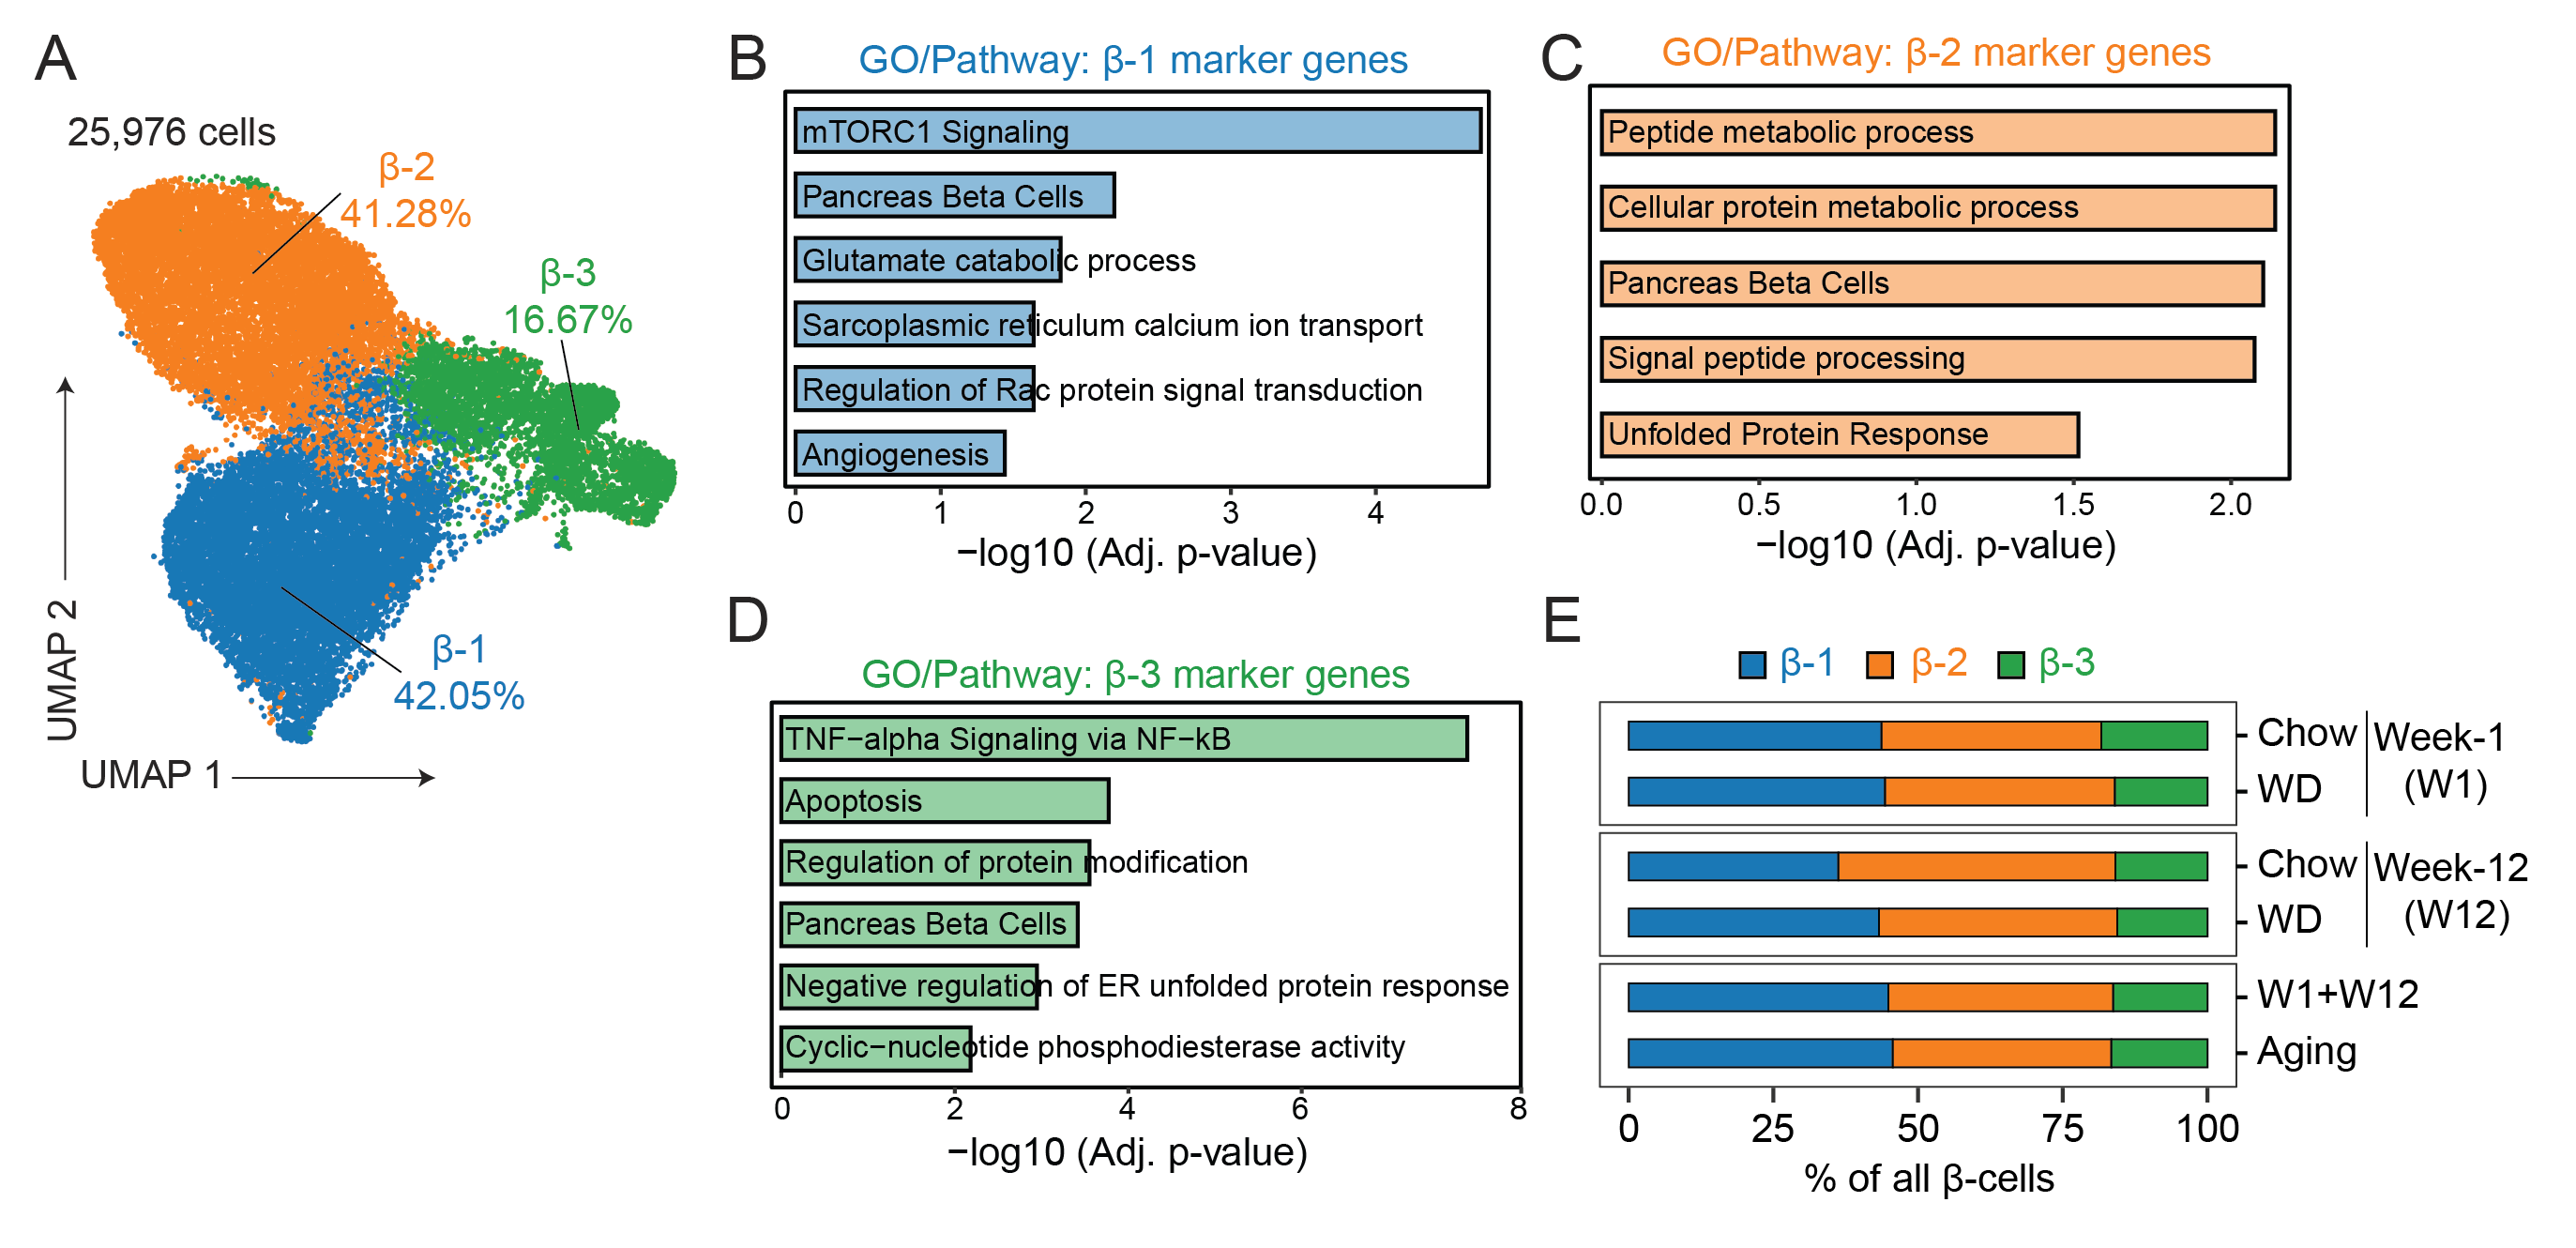
\includegraphics[width=\linewidth]{Chapter4/Fig/F2-12-02.png}
    \caption[Characterization of islet β-cells using scRNA-seq]{\textbf{Characterization of islet β-cells using scRNA-seq.} \textbf{(A)} UMAP embedding of pancreatic islet β-cells, pooled from various time-points (W1, W12, and Aging) and dietary conditions (WD and Chow). Values indicate the overall proportion of each sub-populations, defined based on marker gene expression. \textbf{(B-D)} Enriched gene ontology (GO) terms among marker genes of Beta-1 \textbf{(B)}, Beta-2 \textbf{(C)} and Beta-3 \textbf{(D)}. Significance (-log10 adjusted p value) of the enrichment are shown in bar plots. \textbf{(E)} Relative abundance of β-cell sub-populations computed as a percentage of all β-cells across different experimental conditions based on scRNA-seq data.}
    \label{fig:chp2_betacells1}
\end{figure}

Despite this, considerable changes in the transcriptome were observed across all β-cell sub-populations due to overnutrition and aging. Importantly, both the direction and the magnitude of these changes were similar across the different sub-populations, suggesting uniform responses to these conditions among the β-cell \textbf{(Fig. )}. Based on these observations, we grouped all β-cells together for \gls{dge} analysis, enabling us to identify gene modules. These modules encompass genes that display analogous expression patterns across overnutrition and aging conditions \textbf{(Fig. )}. Importantly, we identified gene clusters that were unique to aging \textbf{(km-9, km-10}, and \textbf{km-2)}, specific to WD intake \textbf{(km-6, km-1, km-8, km-3,} and \textbf{km-7)}, or shared across both conditions \textbf{(km-4} and \textbf{km-5)}. Through gene ontology and pathway analysis \textbf{(Fig. )}, we found that overnutrition and aging typically boosted oxidative phosphorylation (concentrated in km-4), while concurrently weakening the expression of β-cell identity genes (rich in km-5). Changes exclusively linked to the WD involved a significant uptick in the unfolded protein response (enriched in km-6, km-1 and km-8) and a distinct decline in genes linked to alternative splicing (enriched in km-3 and km-7). Aging-centric gene modules had fewer enriched pathways due to the fewer genes within each module. However, we observed an aging-specific decrease in \textit{G6pc2} expression \textbf{(Fig. )} in β-cells, which is in line with their increased glucose sensitivity and enhanced insulin secretion at baseline glucose levels \textbf{(Fig. )}\\\\
Additionally, we identified genes activated by either acute (km-6, mainly seen at W1 of WD intake) or chronic (km-8, more evident at W12 of WD intake) overnutrition. An activation of the \textit{TNFα/NFκB} pathway and an overexpression of genes associated with protein secretion were detected in these two gene modules respectively, shedding light on the islet dysfunction during acute WD intake and the compensatory insulin hyper-secretion during prolonged metabolic stress \textbf{(Fig. )}. Importantly, β-cells acutely responded to \textit{TNFα} one week after WD, reflecting the acute upregulation of \textit{Tnf} expression in Macs-2 in the same stage \textbf{(Fig. )}.\\\\
In conclusion, our analysis established a possible link between beta cell transcriptomic profiles and the inflammation level dictated by islet-associated macrophages, offering mechanistic insights into changes in beta cell function under overnutrition and aging conditions.

% By combining single cell expression profiling and common genetic variation of over one hundred individuals we can begin to assess the impact of genetic variability on expression in a continuous manner across early human development.
% We have imputed genotypes for all of our 125 samples \cite{kilpinen2017common}, so this study allows discovery of single cell eQTL along differentiation. 
% Using the developmental stages just described and methods similar to those described in the previous chapter, we mapped eQTL in each of the \gls{ipsc}, mesendo and defendo populations, yielding 1,833, 1,702 and 1,342 eGenes, respectively. 
% Briefly, we quantified each gene’s average expression level for each donor, experiment, and differentiation stage\footnote{This approach is the same as what is described in the first part of \textbf{Chapter \ref{chapter3}}, and similar to the `dr-mean' described in \textbf{section \ref{sec:best_practice}}, except that the aggregation is done at the experiment level rather than the sequencing run level.}, before using a linear mixed model to test for \textit{cis} eQTL, adapting approaches used for bulk RNA-seq profiles (+ and - 250 kb, MAF >5\% \cite{kilpinen2017common}).\\

% For comparison, we also performed eQTL mapping in cells collected on day1 and day3, i.e. the experimental time points commonly used to identify cells at mesendo and defendo stages \cite{hannan2013production}.
% Interestingly, this approach identified markedly fewer eGenes: 1,181 eGenes at day1, and 631 eGenes at day3.
% These results demonstrate the power of using the single-cell RNA-seq profiles to define relatively homogeneous differentiation stages in a data-driven manner (\textbf{Fig. \ref{fig:endodiff_stage_eqtl}}). 
% Notably, this observation was not merely a consequence of differences in the number of cells or donors considered in each cell population (\textbf{Fig. \ref{fig:endodiff_stage_eqtl}}). \\

% \begin{figure}[h]
% \centering
% \includegraphics[width=14cm]{Chapter4/Fig/endodiff_eqtl.png}
% \caption[eQTL maps of iPSC, mesendo, defendo]{\textbf{Mapping single cell eQTL at different developmental stages.}\\
% (a) Illustration of the single cell eQTL mapping strategy at various stages of differentiation.
% Shown is an example of a defendo-specific eQTL. 
% Box plots of gene expression stratified by the allelic state of
% rs9648854 at each stage, showing an association between rs9648854 and \textit{CNTNAP2} expression at the defendo stage, but not at earlier stages. 
% (b) Comparison of eQTL mapping using different strata of all cells.
% The use of pseudotime-based stages increases the number of detectable eQTL, compared to using the corresponding time point of collection.
% Bar plots represent number of eGenes (genes with at least one eQTL, at FDR < 10\%).
% (c) Similar to b, the number of donors for which gene expression data were assayed at day0, day1, and day3, compared to the number of donors in the pseudotime-inferred mesendo and defendo stages.
% (d) As for (c), with the number of cells.
% \url{https://github.com/ebiwd/EBI-Icon-fonts} by EBI Web Development is licensed under CC BY 4.0. }
% \label{fig:endodiff_stage_eqtl}
% \end{figure}

% Profiling multiple stages of endoderm differentiation allowed us to assess at which stage along this process individual eQTL can be detected as well as the level of sharing of genetic signal across time. 
% We observed substantial regulatory and transcriptional remodelling upon endoderm differentiation of iPSCs, with over 30\% of eQTL being specific to a single stage.
% To define pairwise replication (and conversely specificity) between two sets of test results we considered nominal significance (p value < 0.05) and consistent direction of the effect size.
% Importantly, we observed that stage-specificity of eQTL was not significantly explained by stage-specific gene expression (\textbf{Fig. \ref{fig:endodiff_stage_specific_eqtl}}).
% Our differentiation time course covers developmental stages that have never before been accessible to genetic analyses of molecular traits and thus this study provides the first eQTL maps at mesendoderm and definitive endoderm.
% We next explored whether any of the eQTL identified in these two studies were novel, and found that 349 of them have not been reported in either a recent iPSC eQTL study based on bulk RNA-seq \cite{mirauta2018population}, or in a compendium of eQTL identified from 49 tissues as part of the GTEx project \cite{gtex2017genetic}.
% An eQTL was defined as novel when it was not reported as lead variant (FDR < 10\%) in any of the tissues considered nor was it in \gls{ld} (see \textbf{section \ref{sec:gwas}}) with any reported lead variant, \gls{ld} assessed using $r^2<0.2$.\\

% Finally, we investigated the presence of lead switching events.
% These correspond to two distinct genetic variants that are identified as lead eQTL for the same gene at different stages of differentiation (at LD: $r^2<0.2$),
% We found lead switching events for 155 eGenes (an example in iPSC and defendo is illustrated in \textbf{Fig. \ref{fig:endodiff_stage_specific_eqtl}}). 
% To explore the potential regulatory role of these variants, we investigated whether the corresponding genetic loci also featured changes in histone modifications during differentiation. 
% To do so, we used ChIP-Sequencing to profile five histone modifications that are associated with promoter and enhancer usage (H3K27ac, H3K4me1, H3K4me3, H3K27me3, and H3K36me3) in human embryonic stem cells (hESCs) that were differentiated towards endoderm (using the same protocol employed above) and measured at equivalent time points (i.e. day0, day1, day2, day3, see \textbf{section \ref{sec:endodiff_chipseq}} for detailed experimental methods). 
% Interestingly, we observed corresponding changes in the epigenetic landscape for 20 of the lead switching events (i.e. stage-specific lead variants overlapped with stage-specific changes in histone modification status), suggesting a direct mechanism (\textbf{Fig. \ref{fig:endodiff_stage_specific_eqtl}}).

% \begin{figure}[htbp]
% \centering
% \includegraphics[width=12cm]{Chapter4/Fig/endodiff_stage_specific.png}
% \caption[Stage-specific eQTL]{\textbf{Stage-specific eQTL.}\\
% (a) Proportion of eQTL that are specific to a single stage, shared across two
% stages, or observed across all stages (sharing defined as a lead eQTL variant at one stage with nominal p value < 0.05 and consistent direction
% at another stage).
% (b) Proportion of stage-specific eGenes (genes with a stage-specific eQTL) that are expressed only at a single stage, expressed at two stages, or expressed at all stages. 
% Expressed is defined as normalised log2(CPM+1) > 2. 
% CPM: counts per million.
% (c) A lead switching event consistent with epigenetic remodelling. 
% The overlap of H3K4me1 with the eQTL SNPs across differentiation time points is shown by the coloured bars.}
% \label{fig:endodiff_stage_specific_eqtl}
% \end{figure}

\clearpage

\section{Metabolic stress accelerates aging-induced accumulation of \\CD8\textsuperscript{+} cytotoxic T-cells in the pancreas}
\label{sec:sc_tcells}

In addition to the accumulation of macrophages, our IMC analysis revealed an increase in pancreatic T-cells during both overnutrition and aging conditions (\textbf{Fig.\ref{fig2-10} A}). In particular, we observed an expansion of CD8\textsuperscript{+} activated effector-like T-cells in the pancreas, which was 

\begin{figure}[H]
\centering
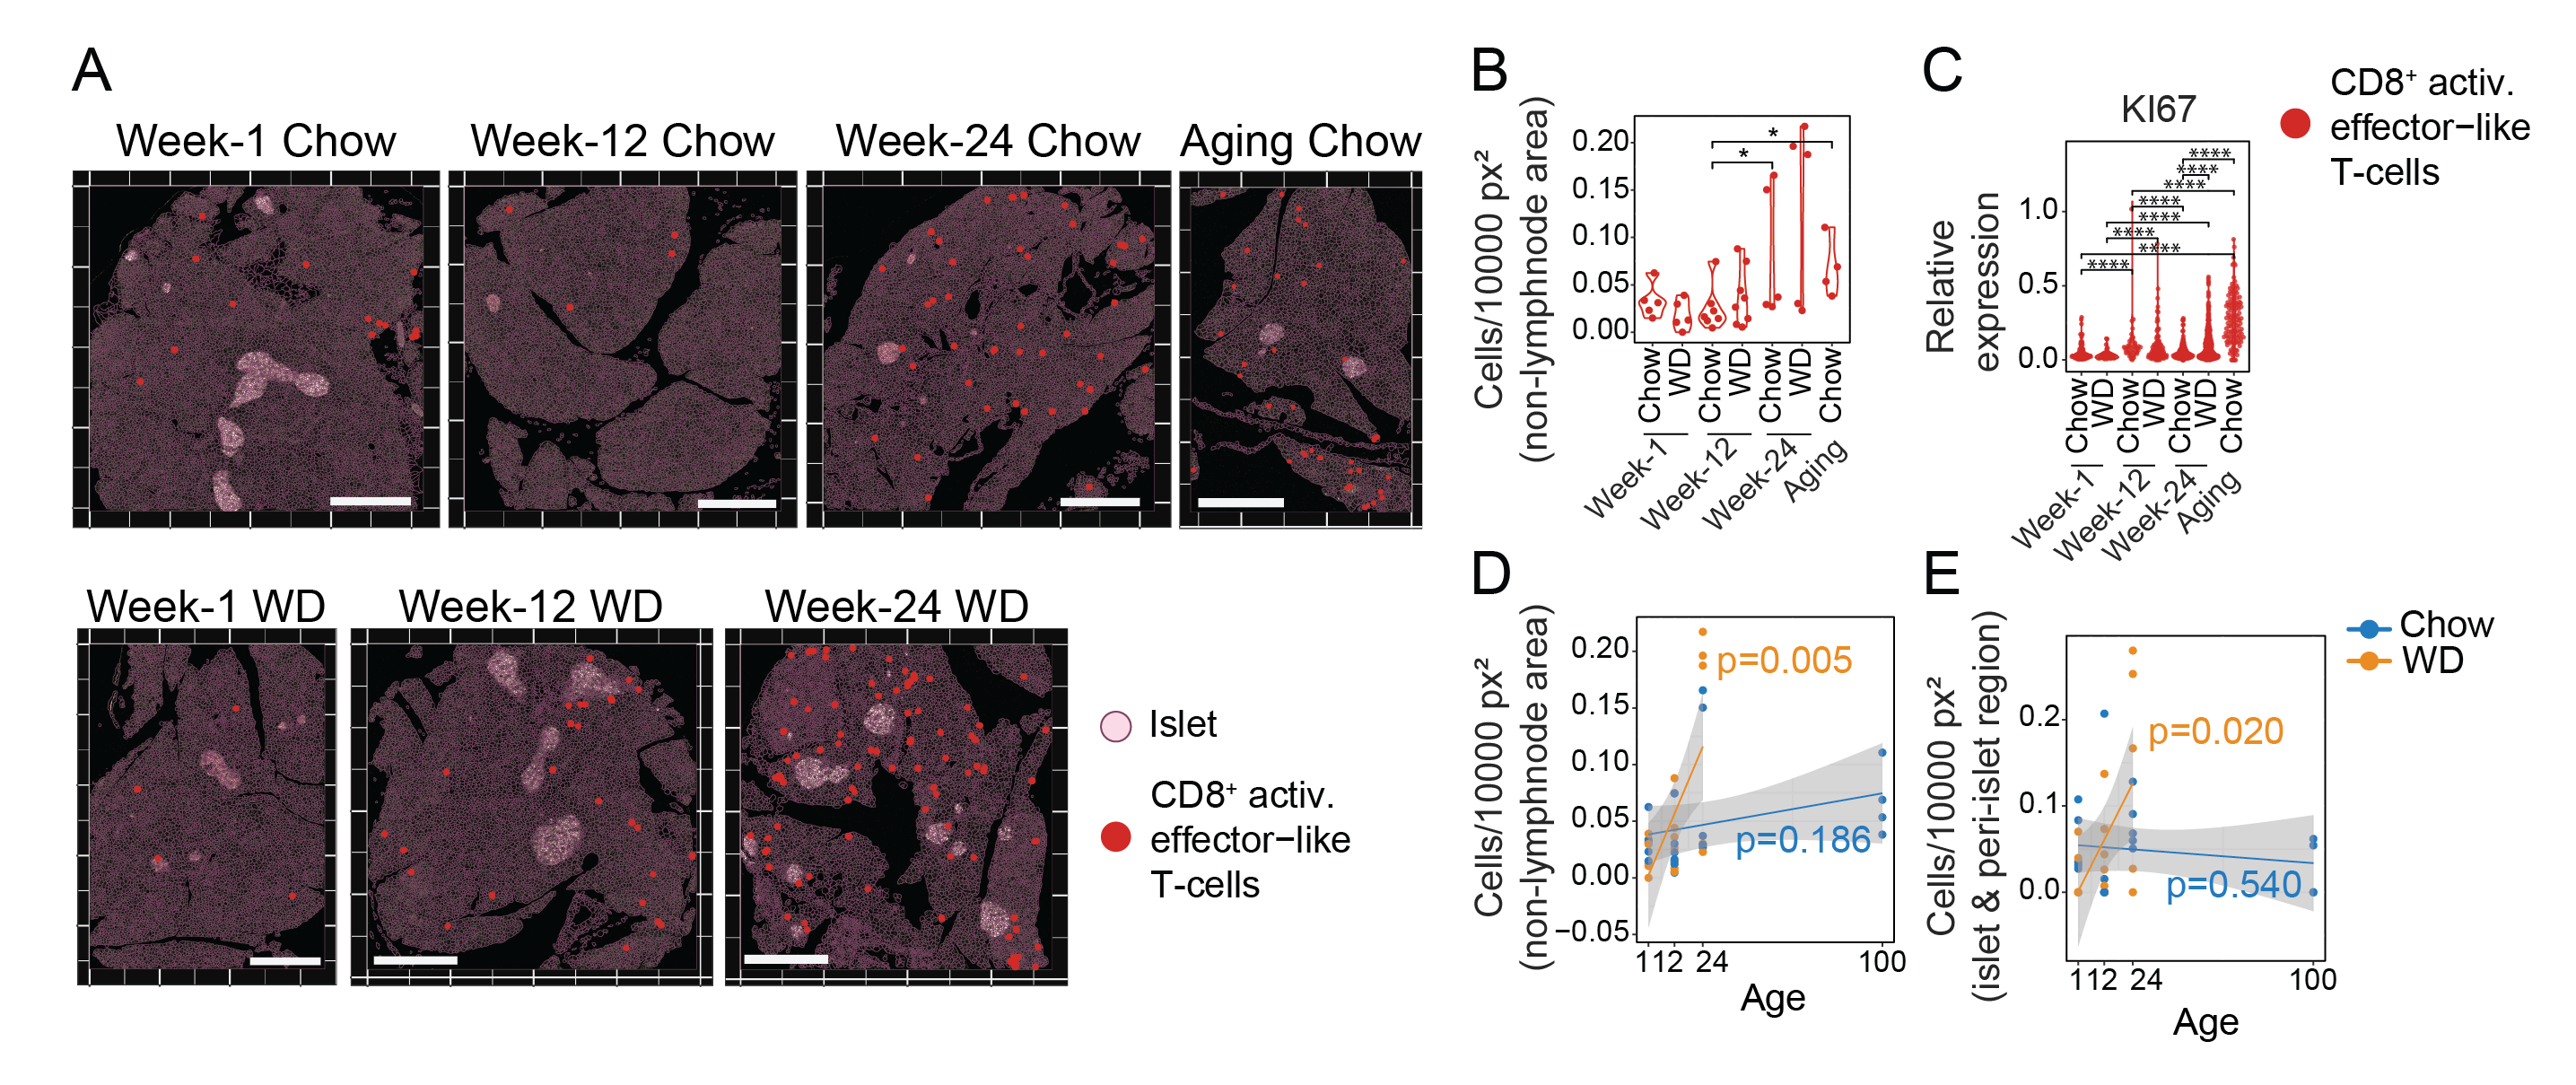
\includegraphics[width=\linewidth]{Chapter4/Fig/F2-10-02.png}
\caption[res-tcells1]{\textbf{Accelerated accumulation of CD8\textsuperscript{+} cytotoxic T-cells in pancreas in response to WD feeeding.} \textbf{(A)} Representative ROIs showing CD8\textsuperscript{+} activated effector-like T-cells in the pancreas. Pancreatic islet regions are marked by raw INS signal (white).  Scale bar 500 μm. \textbf{(B)} Violin plots displaying the densities of CD8\textsuperscript{+} activated effector-like T-cells in non-lymph node pancreatic regions, presented for each mouse across various experimental conditions. * p<0.05. p-values were calculated using the Wilcoxon rank-sum test. \textbf{(C)} Scatter plot showing the density of CD8\textsuperscript{+} activated effector-like T-cells in the pancreas across various time points and feeding conditions. Linear regression fits representing the cell density trends over time are plotted as solid lines. The 95\% confidence intervals for each linear regression are highlighted in grey. Each condition includes data from n $\geq$ 3 mice. p-values for regressions were determined using XX. \textbf{(D)} Violin plot showing \textit{arcsinh} transformed KI67 expression of CD8\textsuperscript{+} activated effector-like T cells across indicated conditions. * p < 0.05, ** p < 0.01, *** p < 0.001 and **** p < 0.0001. p-values were calculated using the Wilcoxon rank-sum test with Bonferroni correction. \textbf{(E)} Scatter plot showing the density of CD8+ activated effector-like T-cells in the pancreatic islet and peri-islet regions across various time points and feeding conditions. Linear regression fits representing the cell density trends over time are plotted as solid lines. The 95\% confidence intervals for each linear regression are highlighted in grey. Each condition includes data from n $\geq$ 3 mice. p-values for regressions were determined using XX. 
}
\label{fig2-10}
\end{figure}

more pronounced under WD feeding (\textbf{Fig.\ref{fig2-10} B,D}). In line with these observations, we found elevated levels of KI67 expression within these T-cells under both WD feeding and aging conditions (\textbf{Fig.\ref{fig2-10} C}). This led us to question whether these CD8\textsuperscript{+} activated effector-like T-cells are further recruited to the pancreatic islets under metabolic and age-induced stress. To investigate this, we analyzed the cell density within the islets and their peripheral regions. We observed significant enrichment of CD8\textsuperscript{+} activated effector-like T-cells in the peri-islet regions under WD conditions, but not during aging (\textbf{Fig.\ref{fig2-10} E}).\\

To gain deeper insights into the dynamics of T-cell sub-populations within the pancreatic islets, we conducted a sub-clustering analysis of our single-cell data, including the total cellular space of non-B-cell lymphocytes (T-cells \& others in \textbf{Fig.\ref{fig2-3} B}). We identified several different T-cell sub-populations, together with other lymphocytes such as innate lymphoid cells (ILC2/3) and natural killer (NK) cells (\textbf{Fig.\ref{fig2-10} F}). It is noteworthy that the major T-cell 

\begin{figure}[H]
\centering
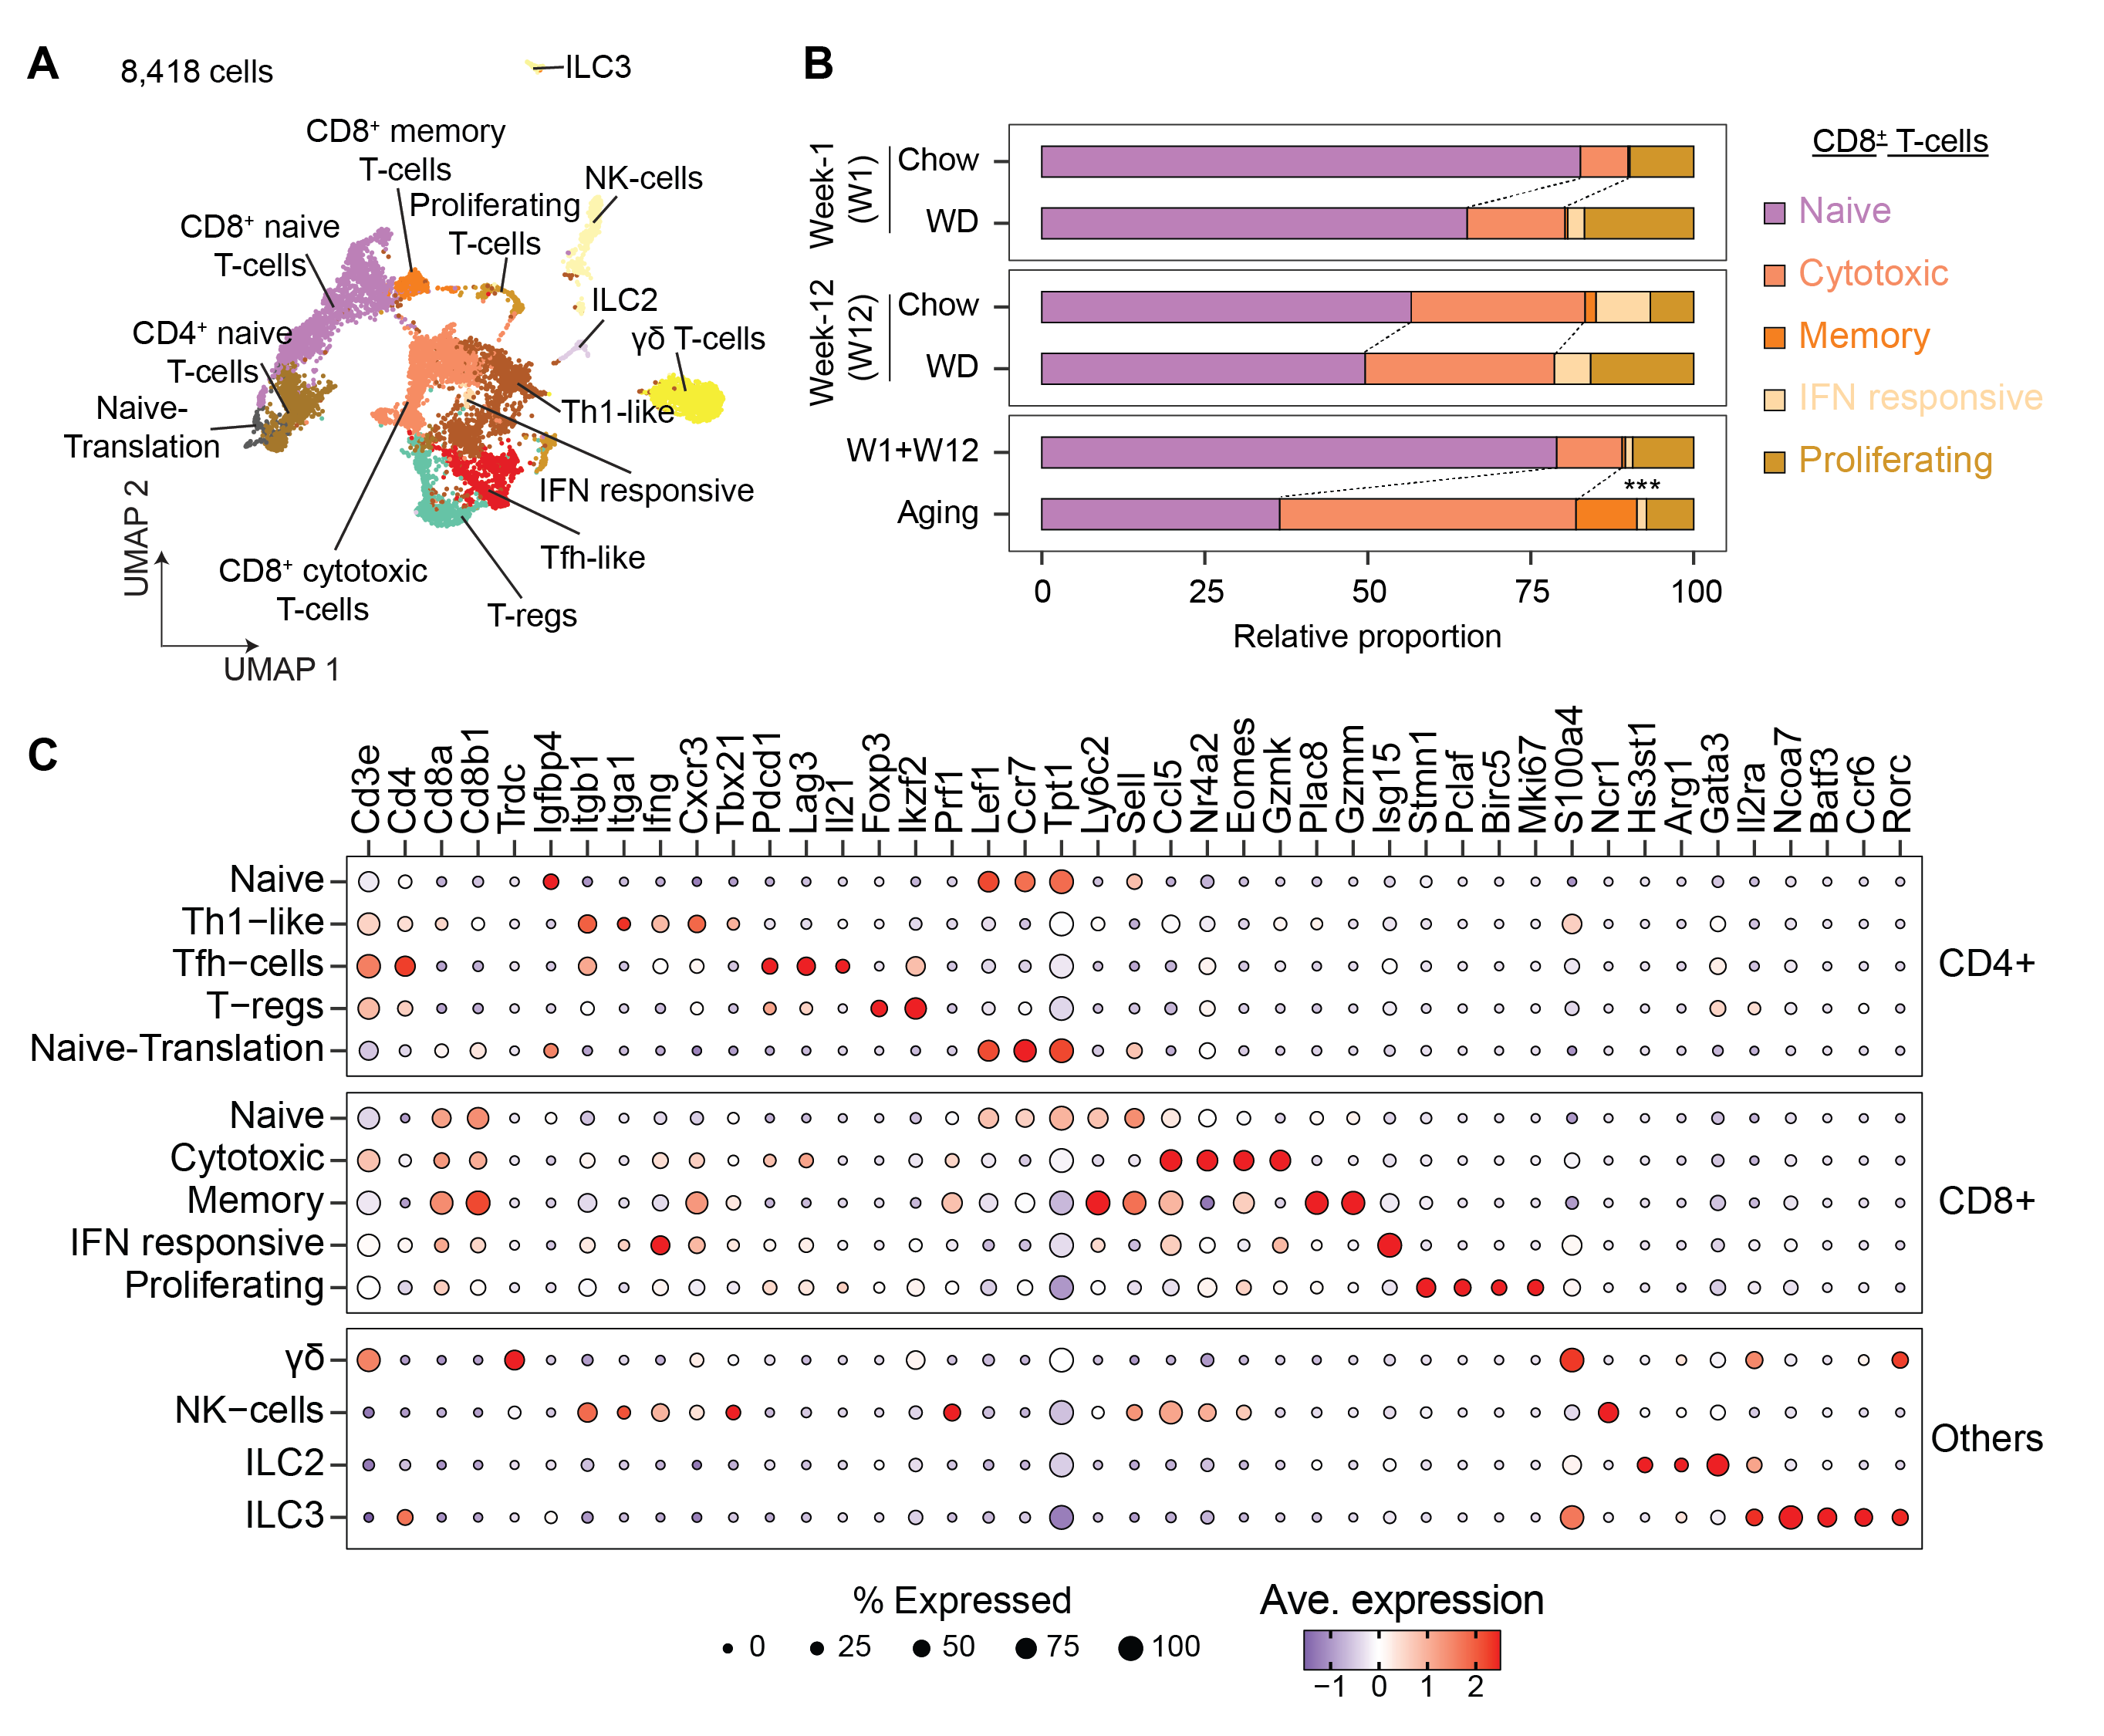
\includegraphics[width=\linewidth]{Chapter4/Fig/F2-10-01.png}
\caption[res-tcells2]{\textbf{Accelerated accumulation of CD8\textsuperscript{+} cytotoxic T-cells in pancreas in response to WD feeeding.} \textbf{(A)} UMAP embedding of islet-associated T- and other lymphocyte populations pooled across the three time-points (W1, W12 and Aging) and two conditions (Chow and WD). Cell types were defined based on marker gene expression. \textbf{(B)} The proportion of each CD8\textsuperscript{+} T-cell sub-population in panel \textbf{(A)}, computed as a percentage of CD8\textsuperscript{+} cells in every experimental group. The cells from different biological replicate cohorts were pooled together. *: p<0.05, **: p<0.01, ***: p<0.001. p values were calculated from a mixed-effects binomial model. \textbf{(C)} Dot-plot showing hallmark genes for all annotated T- and other lymphocyte populations in panel \textbf{(A)}. 
}
\label{fig:chp2_tcells2}
\end{figure}


sub-populations identified within the pancreatic islets from single-cell data mirrored those observed in the whole pancreas from IMC analysis. Based on marker expression, we identified CD8\textsuperscript{+} cytotoxic T-cells, CD8\textsuperscript{+} memory T-cells, and regulatory T-cells (Tregs) within the islets. These subsets exhibit a strong phenotypic alignment with the CD8\textsuperscript{+} activated effector-like T-cells, CD4\textsuperscript{+}/CD8\textsuperscript{+} memory-like cells, and Tregs defined in our IMC data respectively (\textbf{Supp. Fig.\ref{FIG} A}). The whole transcriptomic analysis further augmented our resolution in detecting islet-associated T-cell sub-populations. Notably, we identified two distinct Naive T-cell sub-populations, each manifesting differential CD4 and CD8 expression profiles (\textbf{Fig.\ref{fig2-10} F,H}). This  observation correlates with the mixed CD4\textsuperscript{+}/CD8\textsuperscript{+} non-proliferative silent T-cell cluster defined in our IMC data, which was also characterised by high CD127 but low KI67 protein expression (\textbf{Supp. Fig.\ref{FIG} A}). Both, the scRNA-seq and IMC analyses (\textbf{Fig.\ref{fig2-10} H} and \textbf{Supp. Fig.\ref{FIG} A}) revealed highest EOMES/\textit{Eomes} expression for the CD8\textsuperscript{+} cytotoxic / activated effector-like T-cells. The cytotoxic T-cell subpopulation in the single-cell data was also characterized by high expression of granzyme K (\textit{Gzmk}) and chemokine ligand 5 \textit{Ccl5} (\textbf{Fig.\ref{fig2-10} H}).






% The availability of large numbers of cells per donor across a continuous differentiation trajectory from pluripotent stage to definitive endoderm enabled the analysis of dynamic changes of eQTL strength at fine-grained resolution. 
% To formally test for eQTL effects that change dynamically across differentiation (dynamic eQTL), we tested for associations between pseudotime (both linear and quadratic) and the genetic effect size using allele-specific expression (ASE) and a linear model (see \textbf{Box \ref{box:ase}}):

% \begin{equation}\label{eq:endodiff_ase_pseudotime}
%     \mathrm{ASE} = \alpha_1 \mathrm{pseudotime} + \alpha_2 \mathrm{pseudotime}^2 + \boldsymbol{\psi},
% \end{equation}

% where the genetic effect is defined based on \gls{ase} at the level of single cells, i.e. quantified as fractional read counts overlapping each allele for a given gene-SNP pair (see details in \textbf{Box \ref{box:ase}}).
% We assessed significance using a likelihood ratio test with two degrees of freedoom (i.e. $H_0: \alpha_1 = \alpha_2 = 0$). 
% For this analysis, we focused on the joint set of 4,422 eQTL lead variants (4,470 SNP-gene pairs) discovered at the iPSC, mesendo, and defendo stages and explored how they were modulated by developmental time (using our inferred pseudotime).
% In this way, we uncovered a total of 899 time dynamic eQTL at FDR < 10\%, including a substantial fraction of eQTL that were not identified as stage-specific by the discrete approach previously used (\textbf{page \pageref{fig:endodiff_stage_specific_eqtl}}).
% This analysis is somewhat complementary to the eQTL map perfomed on discrete differentiation stages (\textbf{Fig. \ref{fig:endodiff_stage_eqtl}}), which identified substantial stage-specific effects (\textbf{Fig. \ref{fig:endodiff_stage_specific_eqtl}}).
% Namely, we observe that in general stage-specific effects are weaker and unique to certain cell types.
% In contrast, the dynamic eQTL identified are detected to a certain extent across all cell types, but the strength of the effect is modulated by differentiation time. \\

% One obvious explanation for these subtle dynamic changes could be that they are simply reflecting changes in overall expression. 
% To visualise this, we used a sliding-window approach. 
% Because we need a rather large amount of cells to reliably estimate expression abundance for each individual, we slide a window containing 25\% of the cells along pseudotime by a step of 2.5\% cells.
% In each window, we considered average expression quantifications and estimate genetic effects using eQTL mapping, essentially performing the same analysis we performed in developmental stages in \textbf{section \ref{sec:endodiff_eqtl}}, now in each window.
% In parallel, we reassessed each eQTL in each window taking advantage of the full length transcript sequencing to measure \gls{ase}.
% Here, in each window, we quantified the deviation from 0.5 of the expression of the minor allele at the eQTL (ratio of reads phased to eQTL variants, \textbf{Fig. \ref{fig:endodiff_sliding_window}}). 
% Notably, ASE can be quantified in each cell and is independent of expression level, thus mitigating technical correlations between differentiation stage and genetic effect estimates (\textbf{Box \ref{box:ase}}). 

%****** Box on ASE to quantify genetic effects ******

% \newpage

% \begin{Comment}
% \hspace{-2.5mm}\textbf{Box\ref{box:ase}: Quantifying genetic effects using ASE}\label{box:ase}\\
% \small
% When full-transcript (phased) data is available, \gls{ase} can be used to quantify the genetic effect of a variant on expression as a single ratio, by quantifying the relative expression of one allele over the other.
% For a given eQTL - and the corresponding eQTL variant and eGene -  we i) select individuals that are heterozygous at the eQTL SNP of interest, ii) consider all exonic heterozygous variants on the corresponding eGene, iii) map reads to these SNPs, iv) aggregate all reads coming from the same chromosome and v) compute the ratio. 
% Conventionally, we look at ratios < 0.5 i.e. in the numerator goes the allele with fewer reads mapped to it:

% \vspace{5mm}

% \includegraphics[width=15cm]{Chapter4/Fig/ASE.png}

% If one of these alleles is more responsive to a particular environmental factor (e.g. because of preferential transcription factor binding), then \gls{ase} is expected to vary consistently with that factor. 
% This observation has previously been used to identify GxE interactions in gene expression across individuals \cite{knowles2017allele}. 
% Critically, these \gls{ase} tests are internally matched, because potentially confounding batch effects and technical variation should affect both alleles in each cell similarly.
% Additionally, this test increases power by reducing the number of parameters to estimate, i.e. instead of the standard test for interactions:  

% \begin{equation*}
%     \mathrm{expression} = \sum_{k=1}^{K} \mathbf{e}_k\alpha_k + \mathbf{g}\beta +
%     \sum_{k=1}^{K} \mathbf{g} \odot \mathbf{e}_k\gamma_k + \boldsymbol{\psi},
% \end{equation*}

% where for each of K environments $\mathbf{e}_k$ two terms must be added (to account for E and GxE), resulting in (2*K + 2) parameters needing to be estimated (including one effect size $\beta$ and the variance explained by the noise term $\sigma_n^2$, from $\boldsymbol{\psi} \sim \mathcal{N}(\mathbf{0}, \sigma_n^2\mathbf{I_n})$), we can run:

% \begin{equation*}
%     \mathrm{ASE} = \sum_{k=1}^{K} \mathbf{e}_k\alpha_k + \boldsymbol{\psi}, 
% \end{equation*}
% where we can test directly the effect of the K environments on ASE and therefore only K+1 parameters need estimation (the K $\alpha_k$'s and $\sigma_n^2$).

% \end{Comment}

% \begin{figure}[h]
% \centering
% \includegraphics[width=15.5cm]{Chapter4/Fig/endodiff_running_average.png}
% \caption[Schematic of the sliding window approach]{\textbf{Schematic of the sliding window approach.}\\
% Cells are binned based on pseudotime ordering, to (a) quantify average expression, (b) perform eQTL mapping, and (c) quantify average ASE.
% Each bin includes 25\% of cells, binned at incremental steps of 2.5\%.}
% \label{fig:endodiff_sliding_window}
% \end{figure}

% Both methods result in a measure of genetic effect dynamics, i.e. changing strength of genetic effects along differentiation. 
% Reassuringly, the two approaches were highly consistent across pseudotime (\textbf{Fig. \ref{fig:endodiff_dynamic_eqtl}}).
% To explore this hypothesis, we clustered the top dynamic eQTL (FDR <1\%) jointly based on both the relative gene expression dynamics (global expression changes along pseudotime, quantified in sliding windows as above), and on the genetic effect dynamics (using ASE). 
% This identified four basic dynamic patterns (\textbf{Fig. \ref{fig:endodiff_dynamic_eqtl}}): decreasing early (cluster A), decreasing late (cluster B), transiently increasing (cluster C), and increasing (cluster D). 
% \begin{figure}[htbp]
% \centering
% \includegraphics[width=15.5cm]{Chapter4/Fig/endodiff_pseudo_heatmap.png}
% \caption[Dynamic eQTL]{\textbf{Dynamic eQTL.}\\
% Clustered heatmap of global expression levels, eQTL effect sizes, and ASE across pseudotime for the top 311 genes with the strongest dynamic eQTL effects (FDR < 1\%; out of 785 at FDR < 10\%). 
% For each gene, the dynamic profiles of gene expression and ASE were jointly grouped using clustering analysis, with 4 clusters. 
% The membership of a genes's expression and ASE dynamics to one of these clusters is shown by colours in the right-hand panel. 
% All values in the heatmaps are z-scores, normalised by gene (row). 
% In particular, for ASE, average ASE values are plotted such that red indicates highest deviation from 0.5.
% The diagram in the top right summarises the four identified cluster dynamics, displaying the average dynamic profile of each cluster, computed as the average across z-score normalised gene expression/ASE profiles. 
% Selected examples of the dynamics of allele expression for different cluster-combinations are shown in the bottom right panel.
% Shaded regions indicate standard error (+/- 1 SEM).
% This figure is based on one by Daniel Seaton.}
% \label{fig:endodiff_dynamic_eqtl}
% \end{figure}
% As expected, stage-specific eQTL were grouped together in particular clusters (e.g. defendo specific eQTL in cluster D, \textbf{Fig. \ref{fig:endodiff_dynamic_eqtl_enrichment}}). 
% Notably, the dynamic profiles of gene expression and those of eQTL effects tended to be distinct, demonstrating that expression level is not the primary mechanism controlling variation in genetic effects. 
% In particular, genetic effects were not most pronounced when gene expression was high (\textbf{Fig. \ref{fig:endodiff_dynamic_eqtl}}).
% Distinct combinations of expression and eQTL dynamics result in different patterns of allelic expression over time. 
% This is illustrated by the mesendoderm-specific eQTL for \textit{VAT1L}. 
% Overall expression of \textit{VAT1L} decreases during differentiation, but expression of the alternative allele is repressed more quickly than that of the reference allele (\textbf{Fig. \ref{fig:endodiff_dynamic_eqtl}}). 
% This illustrates how \textit{cis} regulatory sequence variation can modulates the timing of expression changes in response to differentiation, similar to observations previously made in \textit{C. elegans} using recombinant inbred lines \cite{francesconi2014effects}. 
% In other cases, the genetic effect coincides with high or low expression, for example in the cases of \textit{THUMPD1} and \textit{PHC2} (\textbf{Fig. \ref{fig:endodiff_dynamic_eqtl}}). 
% These examples illustrate how common genetic variation is closely linked to the dynamics of gene regulation. 
% % \\

% We next asked whether dynamic eQTL were located in specific regulatory regions. 
% To do this, we evaluated the overlap of our identified dynamic eQTL with epigenetic marks defined using the hESC differentiation time series\footnote{using bulk, at equivalent time points along endoderm differentiation, see \textbf{section \ref{sec:endodiff_chipseq}} for methods.} (\textbf{Fig. \ref{fig:endodiff_dynamic_eqtl_enrichment}}). 
% This revealed an enrichment of dynamic eQTL in enhancer (i.e. H3K27ac and H3K4me1), and promoter (H3K4me3) marks as compared to non-dynamic eQTL (i.e. eQTL we identified which did not display dynamic changes along pseudotime, \textbf{Fig. \ref{fig:endodiff_dynamic_eqtl_enrichment}}), consistent with these SNPs being located in active regulatory elements.

% \vspace{2mm}

% \begin{figure}[htbp]
% \centering
% \includegraphics[width=15cm]{Chapter4/Fig/endodiff_dynamic_enrich.png}
% \caption[Characterisation of dynamic eQTL]{\textbf{Characterisation of dynamic eQTL.}\\
% (a) Summary of the identified cluster dynamics\footnotemark and assignment of stage-specific eQTLs to dynamic eQTL clusters. 
% The numbers of each of the 3 classes of stage-specific eQTL (i.e. iPSC-, mesendo- , and defendo-specific eQTLs) that are assigned to each of the 4 dynamic eQTL clusters.
% (b) Number of genes categorised by the combination of expression and ASE cluster from (a). 
% Average dynamics of expression clusters (rows) and ASE clusters (columns) are shown.
% (c) Overlap of dynamic eQTL variants from a with histone marks.
% The odds ratio compared to the background of all other eQTL variants is shown (*p value < 0.01; **p value < $1x10^{-4}$; Fisher’s exact test).}
% \label{fig:endodiff_dynamic_eqtl_enrichment}
% \end{figure}

% \footnotetext{displaying the average dynamic profile of each cluster, computed as the average values across z-score normalised gene expression/ASE profiles.}

\clearpage

\section{CD8\textsuperscript{+} cytotoxic T-cells receive signals from interferon-\\activated macrophages.}
\label{sec:cell_cell}

% Cells, that make up the tissues, communicate through signaling molecules like ligands and receptors \textbf{\cite{armingol_deciphering_2021,armingol_diversification_2024}}, allowing cells to maintain homeostasis, respond to internal and external perturbations, and enabling proper tissue function. These cell-cell interactions (CCIs) culminate in altered gene expression \textbf{\cite{armingol_deciphering_2021,armingol_diversification_2024}}, and therefore it is crucial to understand how cells interact and communicate, in order to shed light on potential mechanisms underlying biological processes such as development and disease progression. The combination of single-cell transcriptomics and high-confidence \textbf{ligand-receptor interaction (LRI)} databases, has made it possible to infer putative intercellular communications by examining the co-expression of genes corresponding to the ligand-receptor pairs \textbf{\cite{wilk_comparative_2023}}.
% \\\\
As we observed a metabolic stress-induced enhanced accumulation of Type-1 interferon responsive inflammatory macrophages and CD8\textsuperscript{+} cytotoxic T-cells, and since activated macrophages are known to elicit T-cell stimulatory signals \textbf{\cite{}}, we investigated their inter-cellular communication potential by performing ligand-receptor interaction analysis (see Methods for details).

%Disruptions in these cell-cell interactions (CCIs) can lead to disease. Advances in single-cell transcriptomics and ligand-receptor databases now allow for the analysis of these communications, shedding light on the mechanisms behind development and disease progression.


% Cells are able to interact with and influence each other via specific signalling molecules such as ligands (growth factors, chemokines, cytokines), receptors, metabolites, ions, and structural or secreted proteins from the extracellular matrix. \textbf{\cite{armingol_deciphering_2021,armingol_diversification_2024}}. This allows cells to maintain homeostasis, respond to internal and external perturbations, thereby allowing the tissue to function properly. In the absence of proper interactions and coordination, disease ensues. This complex coordination is a result of \textbf{cell-cell interactions (CCIs)} \textbf{\cite{armingol_deciphering_2021}} whereby cells can send or received biochemical and physical signals, that ultimately influence phenotype and function. In particular, interactions mediated through ligands from sender cells and the corresponding cognate receptors on receiver cells are also known as \textbf{cell-cell communication (CCC)}, which culminates in altered gene expression \textbf{\cite{armingol_deciphering_2021,armingol_diversification_2024}}. Therefore, it is crucial to understand how cells interact and communicate, in order to shed light on potential mechanisms underlying biological processes such as development and disease progression. The combination of single-cell transcriptomics and high-confidence \textbf{ligand-receptor interaction (LRI)} databases, has made it possible to infer putative intercellular communications by examining the co-expression of genes corresponding to the ligand-receptor pairs \textbf{\cite{wilk_comparative_2023}}.

% Cells, that make up the tissues, constantly coordinate with each other and their microenvironment.     A plethora of computational tools have been developed to infer CCIs from transcriptomics data. These tools have been reviewed in-depth and extensively bench-marked, and I direct the readers to these publications for further reading \textbf{\cite{armingol_deciphering_2021,armingol_diversification_2024,liu_evaluation_2022,xie_comparison_2023,cheng_review_2023}}

\subsubsection{Intercellular interactions under acute overnutrition}

To investigate the effects of an acute (one week) WD feeding regimen on the intercellular interactions between the sub-populations from the islet-intrinsic macrophages [\textbf{Section \ref{sec:sc_macs}}] in the single-cell data, we performed differential interaction analysis between WD and normal Chow feeding after one week, using CellChat. We excluded the proliferative Macs-4 from the following anaylsis. Through this analysis, we observed an increased number of incoming signals into the inflammatory Macs-3 (\textbf{Fig.\ref{fig2-6} A}) as well as an increase in the incoming interaction strength (\textbf{Fig.\ref{suppl_fig:cell_cell1}, left}), whereas the homeostatic Macs-1 and the \st{other inflammatory} Macs-2 sub-population had down-regulated number of incoming signals (\textbf{Fig.\ref{fig2-6} A}) as well as reduced incoming interaction strength (\textbf{Fig.\ref{suppl_fig:cell_cell1}, left}). We were particularly interested in the inter-cellular communications between the two inflammatory macrophage sub-populations within the islet niche, under acute WD feeding. Therefore, we examined the up- and down-regulated LR signaling pairs from Macs-2 to Macs-3 in the WD compared to normal Chow diet. Several interaction pairs such as cytokine-cytokine receptors, interferon-interferon receptors and TNF-TNF receptors were enriched in response to WD feeding between Macs-2 and Macs-3 (\textbf{Fig.\ref{fig2-6} B}).  Among these, notably, there was a significant enhancement in the signaling from the \textit{Ifnb1} expressing Macs-2 to the Type-1 interferon responsive Macs-3 macrophage sub-population, one week following the initiation of a WD. This communication is characterized by the action of \textbf{IFN-β1} on \textbf{IFN-α} receptors (\textbf{Fig.\ref{fig2-6} B}), which explains the heightened Type-1 interferon response observed in Macs-3 (Figure 4A). Moreover, an increase in the expression levels of Type-1 interferon receptors and their downstream target genes (e.g. \textit{Stat1}) was detected in Macs-3 during the WD (\textbf{Fig.\ref{fig2-6} C}).\\\\In summary, the interplay between the two distinct inflammatory macrophage sub-populations within the islets contributes to the WD-induced activation of the Type-1 interferon response in Macs-3. 

\begin{figure}[!t]
\centering
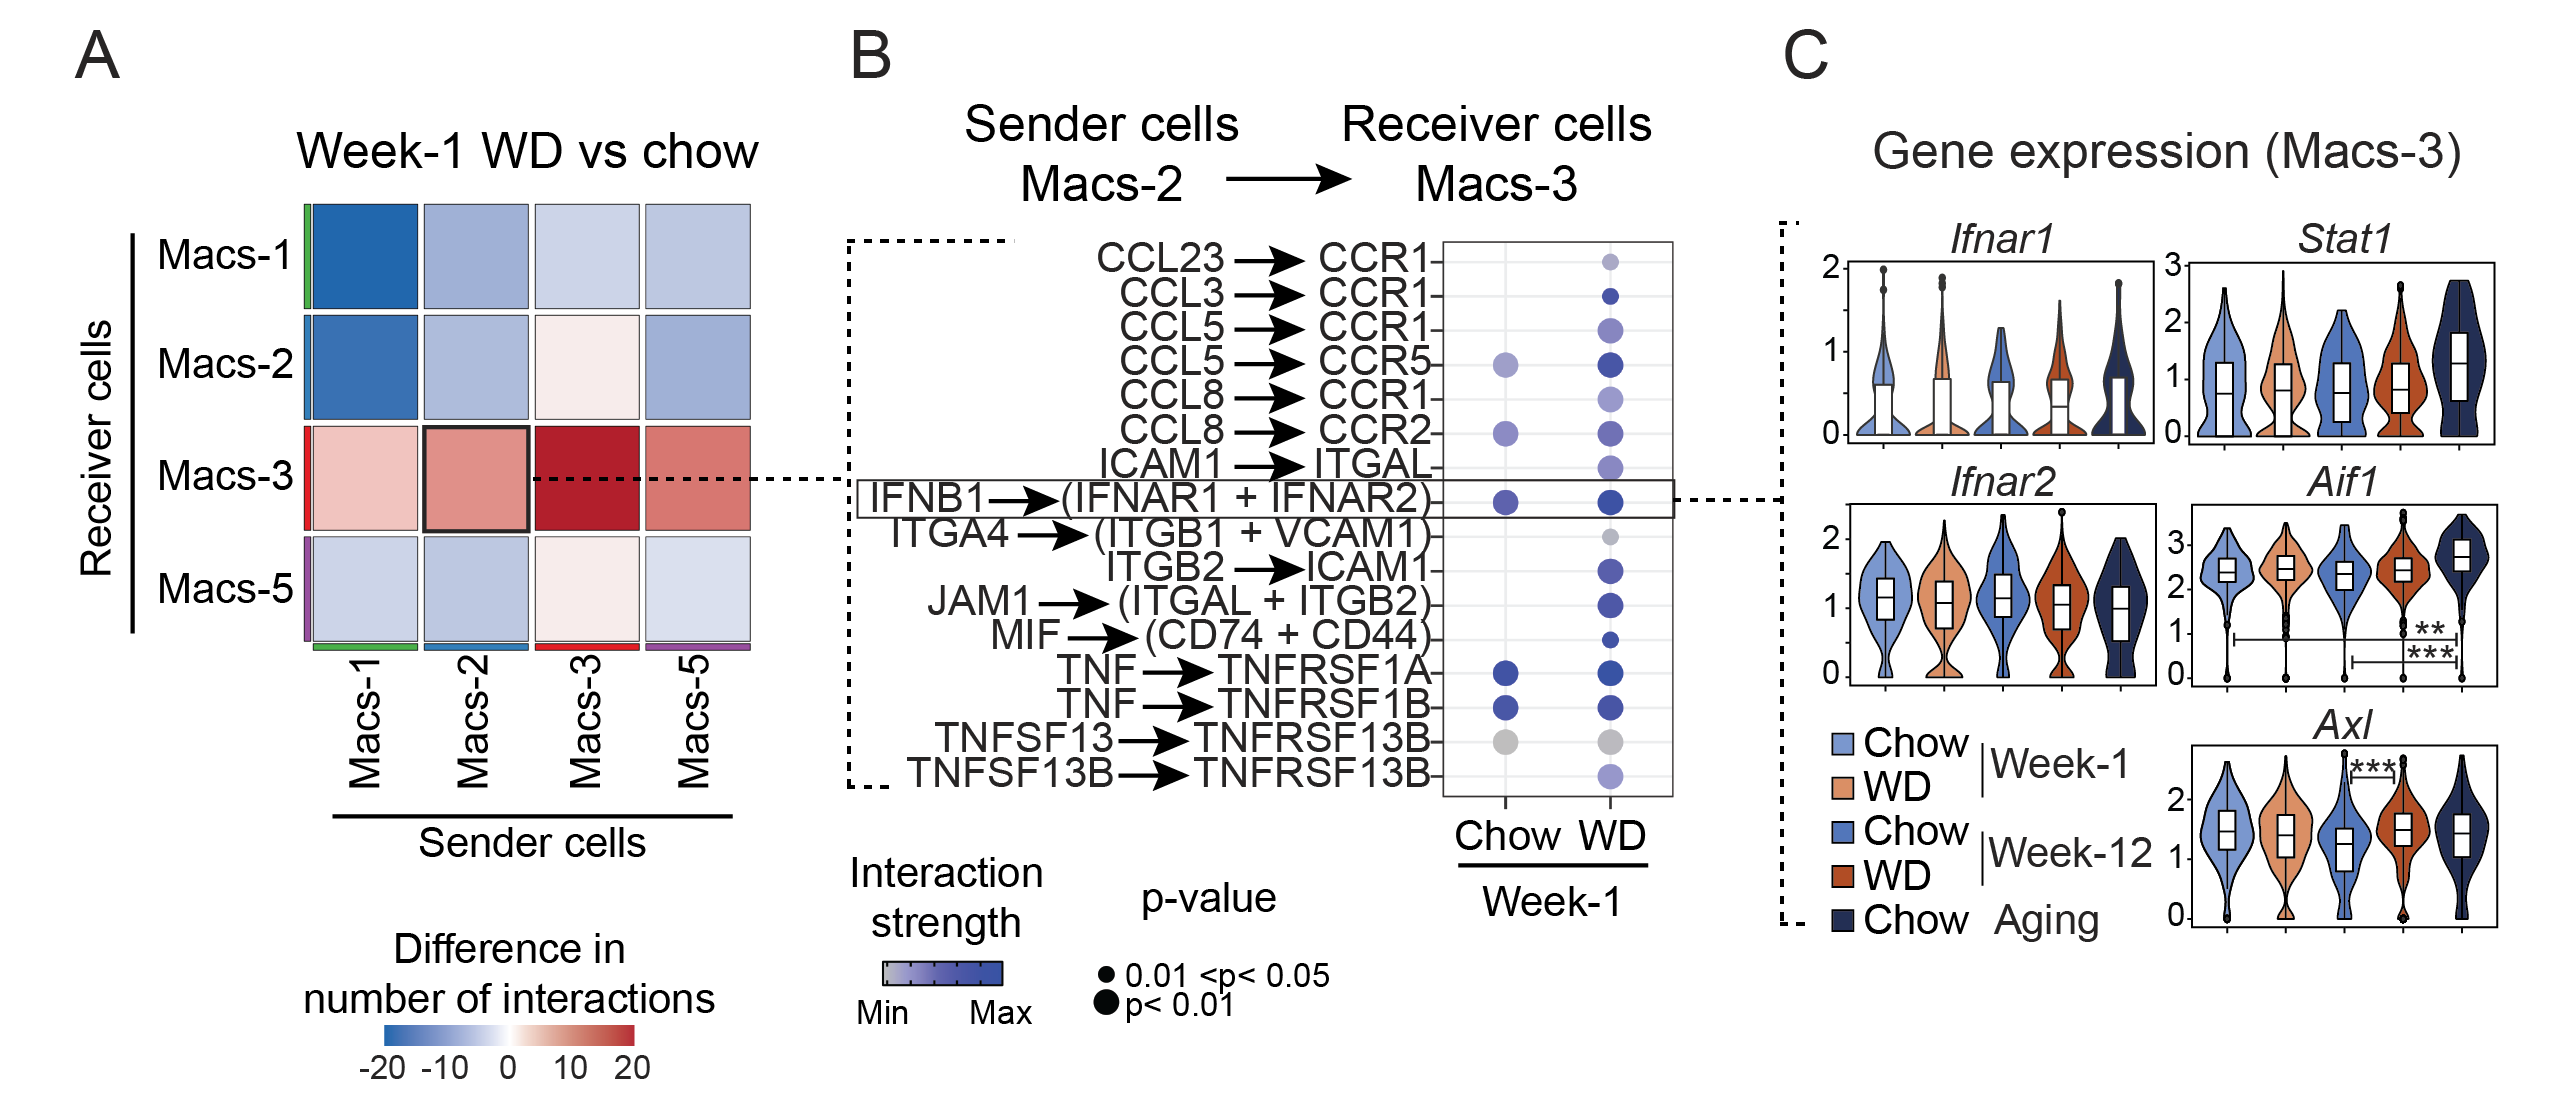
\includegraphics[width=\linewidth]{Chapter4/Fig/F2-6-01.png}
\caption[res-cciw1]{\textbf{Intercellular interactions under acute overnutrition}\\
\textbf{(A)} Heatmap depicting differential number of interactions in the WD cohort (n=2) compared to the Chow (n=3) cohort after 1 week of feeding, between the indicated cell sub-populations. In the color bar, the red (or blue) represents increased (or decreased) number of interactions in the WD data compared to Chow data. Expression of ligand and receptor pairs are accessed in sender and receiver cells respectively. \textbf{(B)} Dot plots depicting ligand-receptor interaction potential, with signals from Macs-2 to Macs-3, under chow and one-week post-WD conditions. The plots highlight all signals that exhibit an increase in interaction intensity in WD-fed group compared to normal Chow. The dot color and size represent the calculated communication probability and significance, respectively. p-values are computed from one-sided permutation test directly within CellChat.\textbf{(C)} Violin plots depicting the normalized expression of potential receptors and associated signaling pathway genes, originating from specified ligand-receptor pairs in Macs-3, across various experimental conditions.
}
\label{fig2-6}
\end{figure}

\subsubsection{Intercellular interactions under chronic overnutrition}
The prolonged exposure to WD feeding necessitates an investigation into its chronic effects on inter-cellular interactions within the islet niche. The sustained overstimulation from a WD is likely to modify the interaction landscape between islet macrophages and T-cells, possibly leading to a persistent inflammatory state. Indeed, local T cells have been shown to play an important role in driving inflammatory processes and insulin resistance by inducing proinflammatory cytokines and chemokines in metabolically active organs, such as the adipose tissue, liver and muscle \textbf{\cite{FIND}}. This promotes recruitment and phenotypic changes of macrophages. Whether such a cellular crosstalk between macrophages and T cells occurs in the pancreas, irrespective of within or around the islets, is unclear.

\begin{figure}[H]
\centering
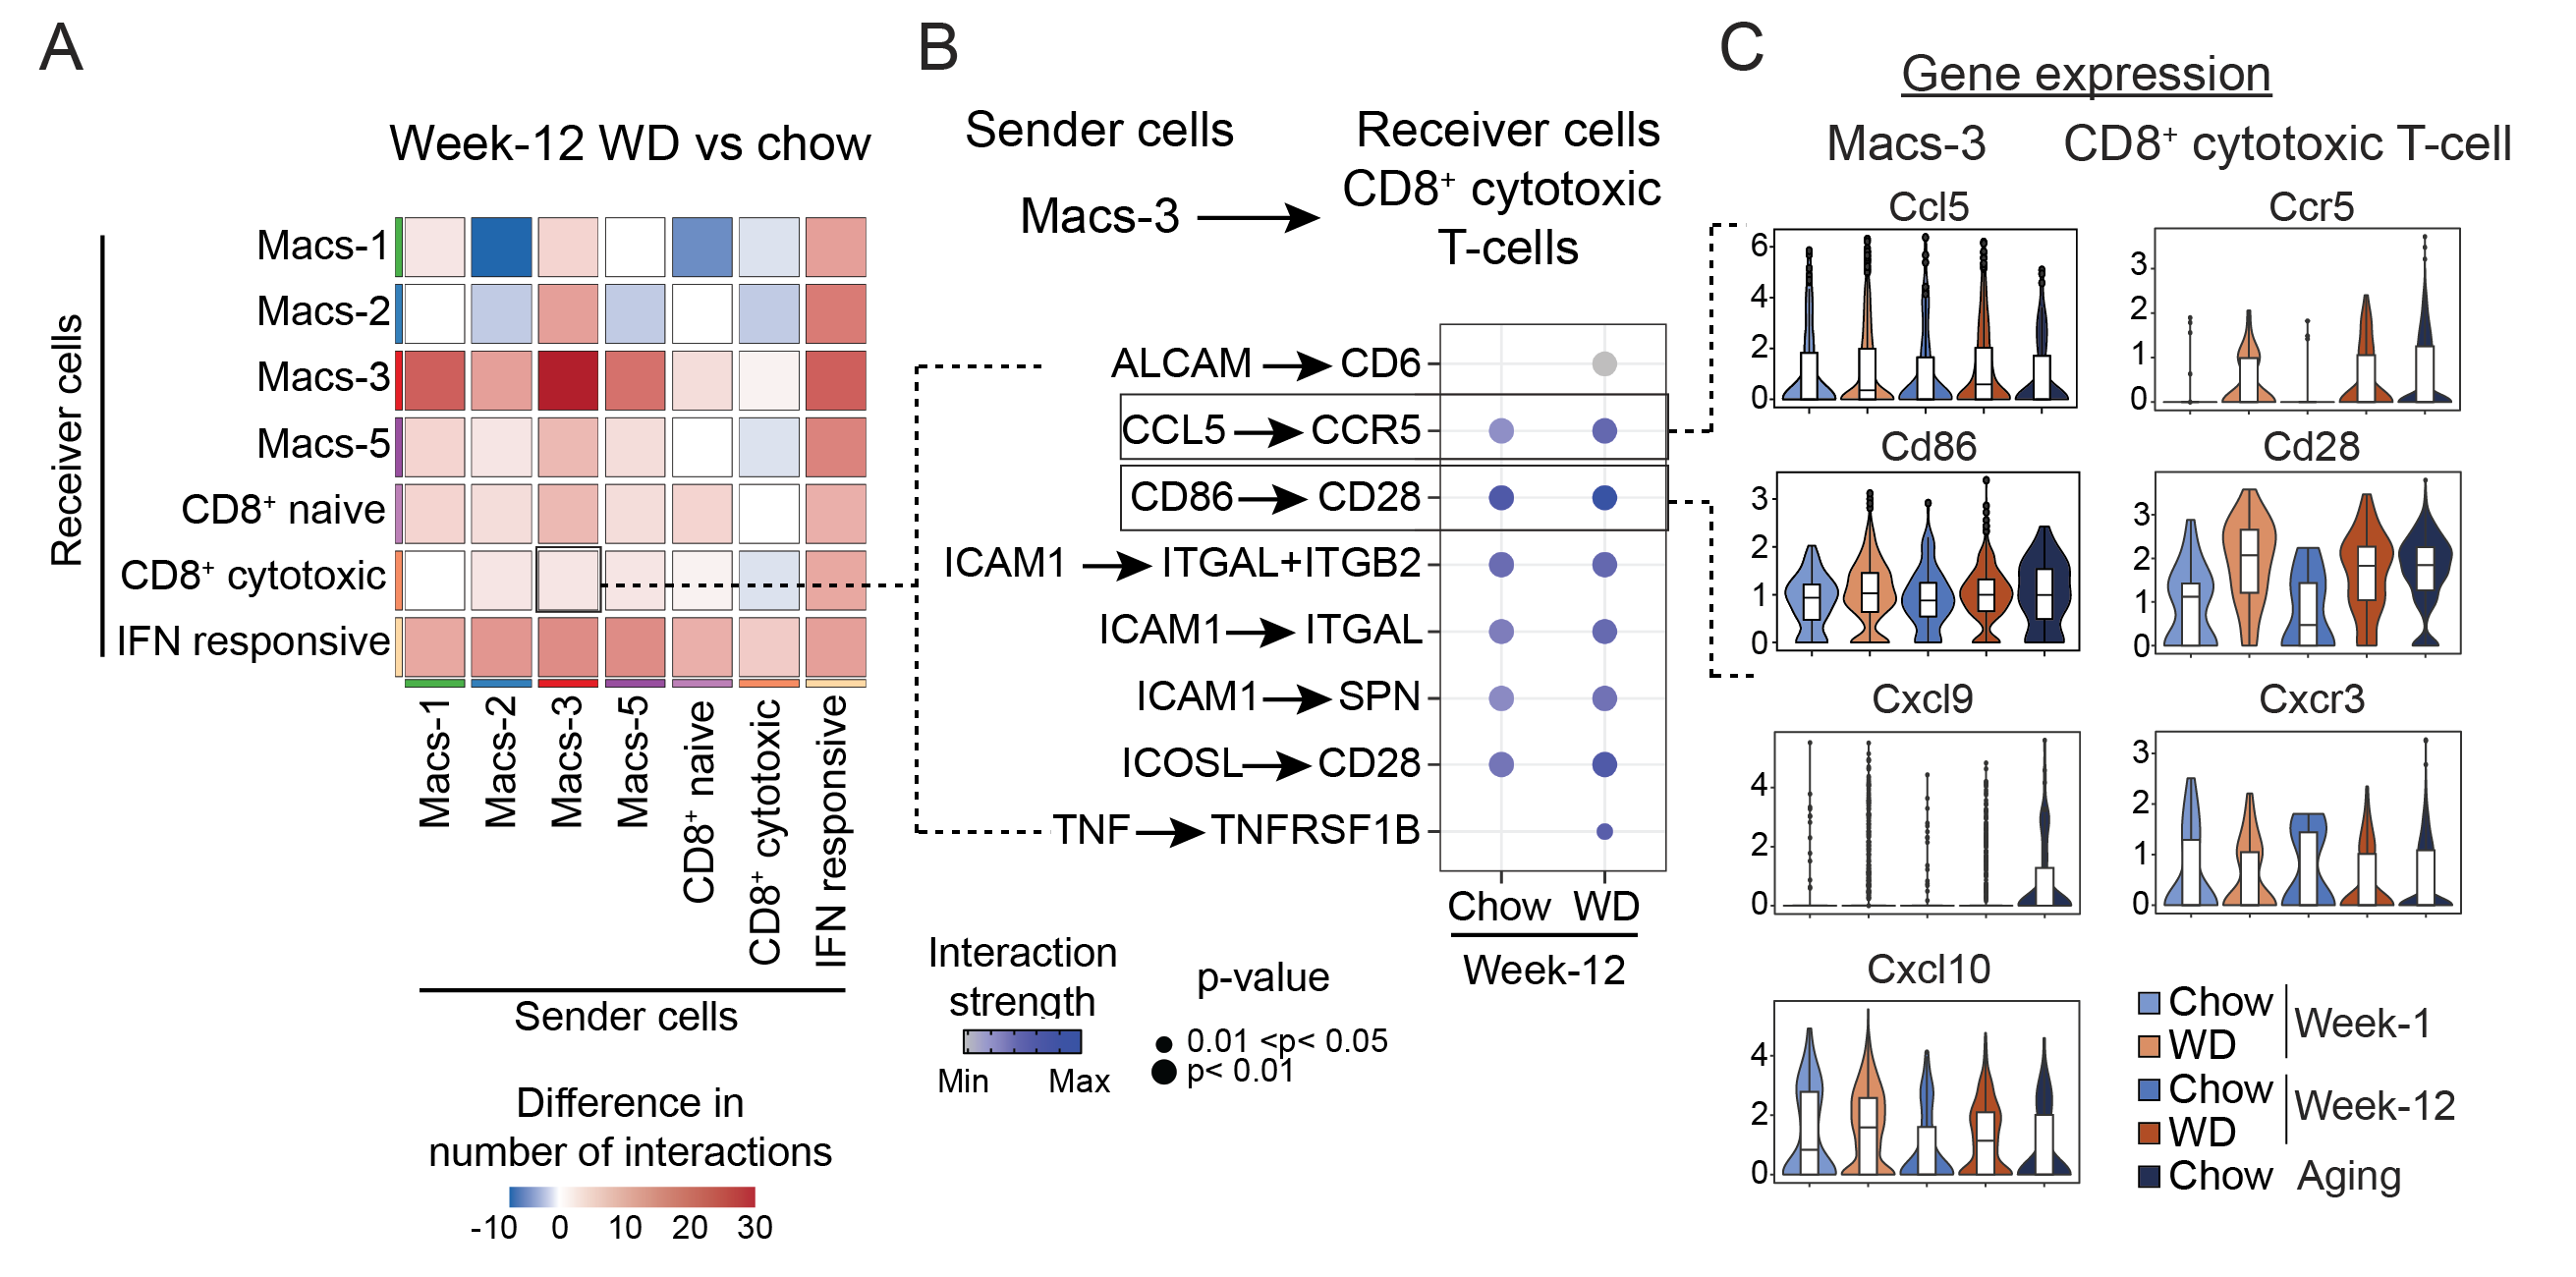
\includegraphics[width=\linewidth]{Chapter4/Fig/F2-7-01.png}
\caption[res-cciw12]{\textbf{Intercellular interactions under chronic overnutrition}\\

}
\label{fig2-7}
\end{figure}

We therefore investigated the chronic effects of WD feeding on the inter-cellular communications within the islets by performing a differential interaction analysis between WD and normal Chow feeding after tweleve weeks, using CellChat. Similar to the prior one-week analysis, we included selected sub-populations from the macrophages and T-cells in the single-cell data. Compared to one-week feeding, the Type-1 IFN-responsive Macs-3 depicted an overall increase in numbers of outgoing and incoming interaction signals (\textbf{Fig.\ref{fig2-7} A}) as well an increase in their corresponding interaction strength (\textbf{Fig.\ref{suppl_fig:cell_cell1}, middle}). To further explore the crosstalk between macrophages and T-cells, we focused on the intercellular interactions between Macs-3 and CD8\textsuperscript{+} cytotoxic T-cells. With the progression of overnutrition, the activated Macs-3 population increased its communication with CD8\textsuperscript{+} cytotoxic T-cells, as evidenced by stronger signals (\textbf{Fig.\ref{fig2-7} B}). Notable interactions between these two sub-populations comprise the action of \textit{Ccl5} secreted by Macs-3 on the \textit{Ccr5} receptor present on CD8\textsuperscript{+} cytotoxic T-cells, as well as the engagement of the co-stimulatory signaling molecules \textit{Cd86} on Macs-3 with \textit{Cd28} on CD8\textsuperscript{+} cytotoxic T-cells (\textbf{Fig.\ref{fig2-7} B}). Within the Macs-3 subset, the expression of \textit{Ccl5} is exclusively triggered by a WD feeding, while CD86 expression was common to both overnutrition and aging (\textbf{Fig.\ref{fig2-7} C}).Additionally, the communication between Macs-3 and CD8\textsuperscript{+} cytotoxic T-cells featured a WD-specific involvement of \textit{Cxcl10}, which acts through the \textit{Cxcr3} receptor on the CD8\textsuperscript{+} cytotoxic T-cells. Conversely, under aging conditions, \textit{Cxcl9} is the preferentially expressed \textit{Cxcr3} ligand (\textbf{Fig.\ref{fig2-7} C}).\\

It is well-established that \textit{Cxcl9} expression is triggered by the canonical Type-1 interferon pathway, whereas \textit{Ccl5} and \textit{Cxcl10} transcription is induced by the non-canonical Type-1 interferon signaling pathway \textbf{\cite{REF}}, reflecting the distinct activation states of Macs-3 under the two different stress conditions (\textbf{Fig.\ref{}}). As mentioned before, the Macs-2 sub-population also showed non-canonical Type-1 interferon responses and up-regulation of \textit{Ccl5} and \textit{Cxcl10} transcription in WD versus control Chow feeding and aging (Figure S4D,E,F). This suggests that cytokine/chemokine-mediated communication between Macs-2/Macs-3 and T-cells significantly differs between overnutrition and aging conditions, even though CD86 and CD28 mediated interactions remain consistent across these scenarios (\textbf{Fig.\ref{suppl_fig:cell_cell2}}). Importantly, our IMC analysis revealed that F4.80- and F4.80low macrophages, corresponding to the Macs-2 and Macs-3 subtypes, respectively, show a positive correlation with CD8\textsuperscript{+} activated effector-like T-cells in the pancreatic tissue indicating a mutual dependency (\textbf{Fig.\ref{fig2-8} A}). Additionally, CD8\textsuperscript{+} and CD11c\textsuperscript{+} cells were frequently observed, both in the exocrine pancreas and within pancreatic islets (\textbf{Fig.\ref{fig2-8} B}), further underscoring the presence of pancreas tissue-resident T-cells and myeloid cells.  


\begin{figure}[H]
\centering
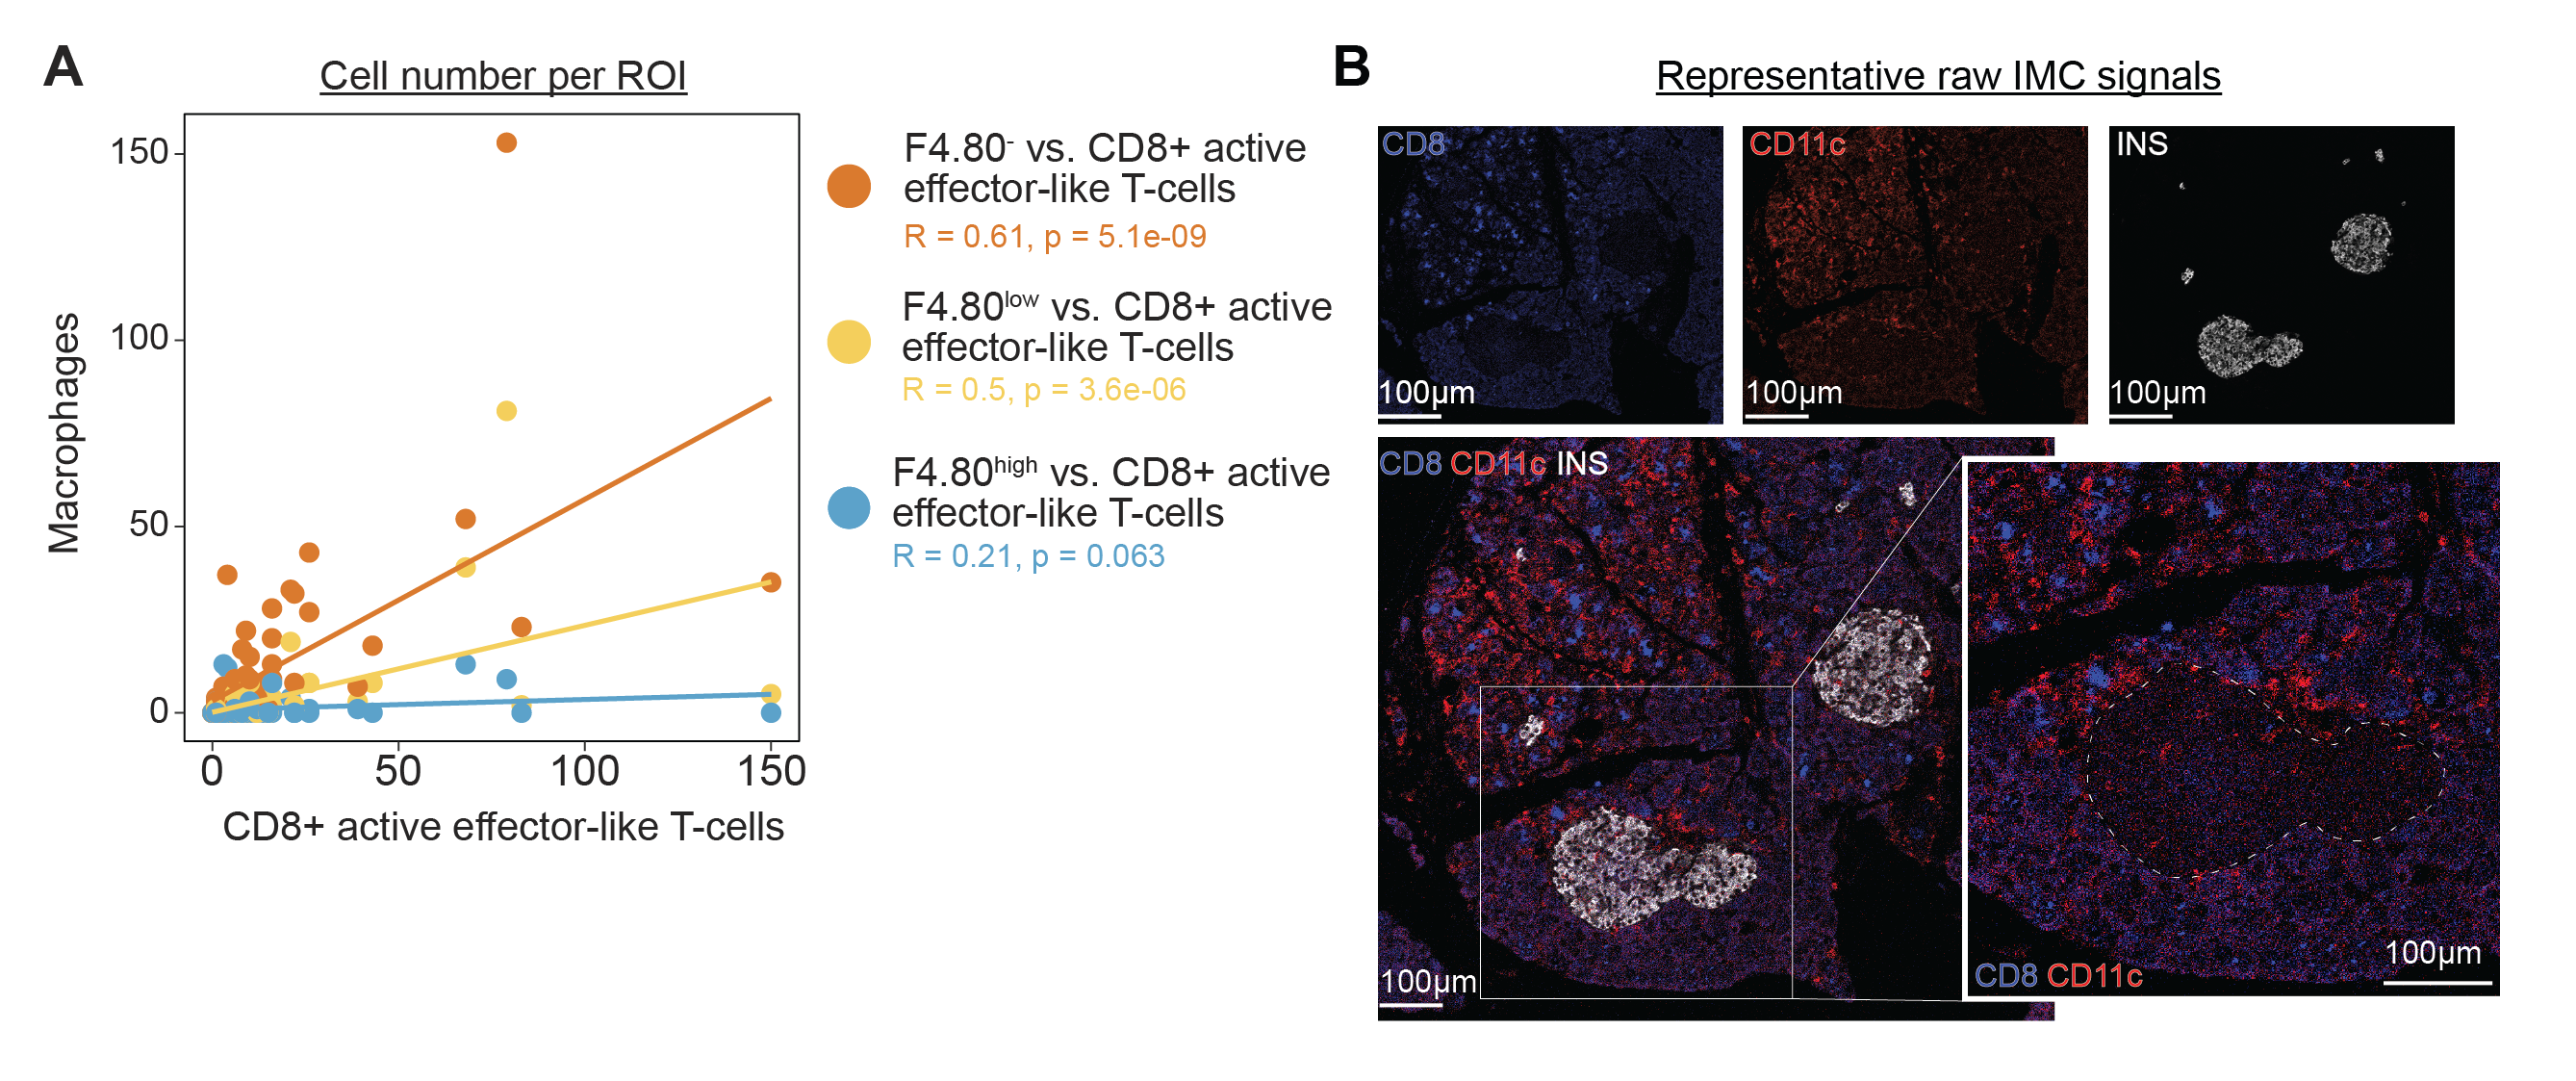
\includegraphics[width=\linewidth]{Chapter4/Fig/F2-8-01.png}
\caption[res-cci-imc]{\textbf{Co-Localization of Macrophages and T-Cells}\\
\textbf{(A)} Scatter plot depicting the Pearson correlation between the counts of CD8\textsuperscript{+} activated effector-like T-cells and three macrophage sub-populations within the same ROIs. Solid lines represent best fit in each correlation analysis. Pearson correlation coefficients and p-values for the corresponding macrophage sub-populations are included. \textbf{(B)} Representative ROI showing raw signals from the CD8 (blue), CD11c (red), and INS (white) channels. Scale bar, 100 µm.}
\label{fig2-8}
\end{figure}

%mouse pancreatic islets, we performed differential interaction analysis between   An up-regulation in intercellular communication among various immune cell sub-populations was observed in response to both acute (Figure 7A; Figure S7A) and chronic (Figure 7D; Figure S7A) overnutrition conditions. Notably, 
